\documentclass[titlepage,letterpaper,final]{scrartcl}

\usepackage{scrindex}           % multiple index support using the "index" package
\usepackage{index}

% This file contains macros included in manual.tex and forcing.tex, in the preamble.
% This way we have all the URLs and such in one place.

%% THE FOLLOWING SHOULD CHANGE FOR A STABLE RELEASE:
\newcommand{\PISMREV}{revision \texttt{@Pism_REVISION_TAG@}}
\newcommand{\PETSCREL}{3.2}
\newcommand{\PISMDOWNLOADMSG}{Get development branch source code:
  \quad \texttt{git clone -b dev git@github.com:pism/pism.git pism-dev} \quad}
\newcommand{\PISMBROWSERURL}{http://www.pism-docs.org/wiki/doku.php?id=browser}
\newcommand{\PISMEMAIL}{\href{mailto:help@pism-docs.org}{\texttt{help@pism-docs.org}}}

\newcommand{\normalspacing}{\renewcommand{\baselinestretch}{1.1}\tiny\normalsize}
\newcommand{\tablespacing}{\renewcommand{\baselinestretch}{1.0}\tiny\normalsize}
\normalspacing

\usepackage[usenames]{xcolor}

\usepackage{bm,url,xspace,verbatim}
\usepackage{amssymb,amsmath}
\usepackage[pdftex]{graphicx}

\usepackage{booktabs}           % better rules in tables
\usepackage[nohyphen]{underscore}

\newcommand{\ddt}[1]{\ensuremath{\frac{\partial #1}{\partial t}}}
\newcommand{\ddx}[1]{\ensuremath{\frac{\partial #1}{\partial x}}}
\newcommand{\ddy}[1]{\ensuremath{\frac{\partial #1}{\partial y}}}
\renewcommand{\t}[1]{\texttt{#1}}
\newcommand{\Matlab}{\textsc{Matlab}\xspace}
\newcommand{\bq}{\mathbf{q}}
\newcommand{\bU}{\mathbf{U}}
\newcommand{\eps}{\epsilon}
\newcommand{\grad}{\nabla}
\newcommand{\Div}{\nabla\cdot}

%% macros having to do with documentation for options; note these appear in the index

\newindex{default}{idx}{ind}{General Index}
\newindex{options}{odx}{ond}{PISM Command-line options}

\def\optsection#1{%
  \def\optindex##1{\index[options]{#1!##1}}
  \def\optseealso##1{\index[options]{#1|see{##1}}}
}

\optsection{FIXME}

% Use this to index option definitions:
\newcommand{\intextoption}[1]{\texttt{-#1}\optindex{\texttt{-#1}}}

\newcommand{\txtopt}[2]{\texttt{-#1} #2\optindex{\texttt{-#1} #2}}

\newcommand{\listopt}[1]{\txtopt{#1}{\emph{comma-separated list}}}
\newcommand{\fileopt}[1]{\txtopt{#1}{\emph{filename}}}
\newcommand{\timeopt}[1]{\txtopt{#1}{\emph{range or list}}}

\def\variable#1{\texttt{#1}\index{NetCDF variables!\texttt{#1}}}
\def\config#1{\texttt{#1}\index{Configuration flags and parameters!\texttt{#1}}}
\def\class#1{\texttt{#1}\index{C++ classes!\texttt{#1}}}


%\addtolength\topmargin{-.1in}
\addtolength\textheight{0.75in}
\addtolength{\oddsidemargin}{-.4in}
\addtolength{\evensidemargin}{-.4in}
\addtolength{\textwidth}{0.9in}

%% uncomment to see locations of index entries
% \proofmodetrue

% this lets us avoid the scrartcl/hyperref conflict...
\let\ifvtex\relax

% hyperref should be the last package we load
\usepackage[pdftex,
colorlinks=true,
plainpages=false, % only if colorlinks=true
linkcolor=blue,   % only if colorlinks=true
citecolor=blue,   % only if colorlinks=true
urlcolor=blue     % only if colorlinks=true
]{hyperref}

\pdfinfo{
/Title (PISM User's Manual)
/Author (the PISM authors)
/Subject (Using PISM, a Parallel Ice-Sheet Model)
/Keywords (PISM ice sheet modeling)
}

\begin{document}
\graphicspath{{figs/}}

\begin{titlepage}

  \begin{center}

    \includegraphics[width=3.3in,keepaspectratio=true]{pism-logo}

    \vspace{2.0cm}
    {\huge \usekomafont{title} User's Manual}
    \vspace{2.0cm}

    \includegraphics[width=4.2in,keepaspectratio=true]{grn-1km-csurf}
    \vfill

    \small Support by email: \PISMEMAIL.
    \medskip

    Manual date \today. Based on PISM \PISMREV.
    \medskip

    \PISMDOWNLOADMSG
  \end{center}
\end{titlepage}

\newpage
\phantom{bob}

\centerline{\textsc{Authorship}}
\bigskip

\normalspacing
PISM is a joint project between developers in the ice sheet modeling group at the University of Alaska (UAF), developers at the Potsdam Institute for Climate Impact Research (PIK), and several additional developers listed here.  Current (or recent) affiliation and area of contributions shown:
\bigskip
\normalspacing

\renewcommand{\arraystretch}{1.3}
\begin{tabular}{ll}
\textbf{Torsten Albrecht (PIK)} & ice shelf physics and numerics \\
\textbf{\underline{Andy Aschwanden} (UAF)} & \begin{minipage}[t]{4in} scripts, visualization, thermodynamics, SeaRISE-Greenland, Storglaci\"aren  \end{minipage}  \\
\textbf{Jed Brown (ANL)} & source code original author, SSA numerics, PETSc underpinnings \\
\textbf{\underline{Ed Bueler} (UAF)} & \begin{minipage}[t]{4in} principal investigator, verification, earth deformation, SIA numerics, thermodynamics, documentation  \end{minipage} \\
\textbf{Dani DellaGiustina (UAF)} & regional tools and modeling \\
\textbf{Johannes Feldman (PIK)} & marine ice sheet processes \\
\textbf{Bob Fischer (GFDL)} & coupling design \\
\textbf{Marijke Habermann (UAF)} & inversion\\
\textbf{Marianne Haselhoff (UBC)} & ice streams: physics and numerics\\
\textbf{Regine Hock (UAF)} & surface mass and energy balance \\
\textbf{\underline{Constantine Khroulev} (UAF)} & \begin{minipage}[t]{4in} source code primary author, input/output, software design, climate couplers, parallelization, testing, user support, most documentation, most bug fixes, regional tools, \dots \end{minipage} \\
\textbf{Anders Levermann (PIK)} & calving, ice shelf processes \\
\textbf{Craig Lingle (UAF)}\index{People!Lingle, Craig} & original SIA model, earth deformation \\
\textbf{Maria Martin (PIK)} & SeaRISE-Antarctica, Antarctica processes \\
\textbf{Mattias Mengel (PIK)} & marine ice sheet processes \\
\textbf{David Maxwell (UAF)} & inversion, SSA finite elements, python bindings \\
\textbf{Ward van Pelt (IMAU)} & hydrology analysis and design \\
\textbf{Julien Seguinot (INK)} & bug fixes \\
\textbf{Ricarda Winkelmann (PIK)} & Antarctica processes, coupling, and modeling  \\
\textbf{Florian Ziemen (MPI)} & bug fixes, sliding \\
\end{tabular}

\bigskip
\noindent Email the \underline{underlined} UAF developers at \qquad \PISMEMAIL.

\bigskip\bigskip
\noindent \textsc{Front page}:  Magnitude of horizontal surface velocity from PISM run on a horizontal grid resolution of 1\,km.  Visualization by IDV.

\vfill

\newpage
\vspace{0.2in}
\begin{quote}
\textsl{Copyright (C) 2004--2013 The PISM Authors}
\medskip

\noindent \textsl{This file is part of PISM.  PISM is free software; you can redistribute it and/or modify it under the terms of the GNU General Public License as published by the Free Software Foundation; either version 3 of the License, or (at your option) any later version.  PISM is distributed in the hope that it will be useful, but WITHOUT ANY WARRANTY; without even the implied warranty of MERCHANTABILITY or FITNESS FOR A PARTICULAR PURPOSE.  See the GNU General Public License for more details.  You should have received a copy of the GNU General Public License\index{GPL (\emph{GNU Public License})} along with PISM; see \emph{\texttt{COPYING}}.  If not, write to the Free Software Foundation, Inc., 51 Franklin St, Fifth Floor, Boston, MA  02110-1301 USA}
\end{quote}
\vspace{0.5in}

\centerline{\textsc{Acknowledgements}}
\bigskip

\small
The NASA Modeling, Analysis, and Prediction program\index{Organizations!NASA!Modeling, Analysis, and Prediction Program} (grant \# NNX09AJ38G) supports the development of PISM from 2009 to 2013.  Development from 2002 to 2008 was supported by the NASA Cryospheric Sciences Program\index{Organizations!NASA!Cryospheric Sciences Program}.  The Snow, Ice, and Permafrost (SIP) group\index{Organizations!Geophysical Institute!Snow, Ice, and Permafrost group} at the Geophysical Institute is the home for the University of Alaska PISM developers; find us in Elvey 410D.  The Arctic Region Supercomputing Center\index{Organizations!Arctic Region Supercomputing Center (ARSC)} has provided significant computational resources and technical help in the development of PISM.

Thanks for comments/questions from many PISM users around the world, including these not already listed as contributors:

\begin{quote}
Tolly Adalgeirsdottir, Antje Fitzner, Nick Golledge, Tore Hattermann, Marianne Madsen, Malou Maris, Tim Morey, Mirena Olaizola, Christian Rodehacke, Nathan Shemonski, Sebastian Simonsen, Anne Solgaard, Ben Sperisen, Synne H\o{}yer Svendsen, Martin Truffer, Shuting Yang, Ryan Woodard
\end{quote}

\noindent for helpful comments and questions on PISM and this \emph{Manual}.  Dave Covey, Don Bahls, and Greg Newby have supported our hardware, software, and computations.  Bob Bindshadler, Sophie Nowicki, Jesse Johnson, and others in the SeaRISE group have motivated and assisted PISM development in many ways.  

\normalsize



\newpage
\setcounter{tocdepth}{3}
\small
\tableofcontents
\normalsize

\newpage


\section{Introduction}\label{sec:intro}

Welcome!  All information about PISM is online at the home page
\begin{center}
  \url{http://www.pism-docs.org}
\end{center}
Please see the extensive lists of PISM publications and applications at that page.

This User's Manual gives examples of how to run PISM using publicly-available data for: the whole Greenland ice sheet, the Jakobshavn outlet glacier in Greenland, the Ross ice shelf in Antarctica, and the St\"orglaciaren mountain glacier in Sweden.  It documents all the PISM options.  It summarizes the continuum models used by PISM, and it illustrates how PISM's numerical approximations are verified.

See the PISM Installation Manual\footnote{PDF for latest stable release at \url{http://www.pism-docs.org/wiki/lib/exe/fetch.php?media=installation.pdf}.}
for how to download\index{PISM!download source code} the PISM source code and install
it\index{PISM!install}, along with needed libraries.  The PISM Climate Forcing
Manual\footnote{PDF for latest stable release at \url{http://www.pism-docs.org/wiki/lib/exe/fetch.php?media=forcing.pdf}.}
extends the User's Manual to cover additional couplings to atmosphere and ocean
models and data.

Users who want to understand more deeply how PISM is designed, or who want to extend it,  will need to go beyond what is described here.  See the \emph{Source Code Browser}\index{PISM!\emph{Source Code Browser (HTML)}}, which is online for the latest stable version.\footnote{At \url{http://www.pism-docs.org/wiki/doku.php?id=browser}.}  It can be generated from source code as described in the PISM Installation Manual.  It gives a complete view of the class/object structure of the PISM source code.


\vspace{.3in}
  
\begin{center}
\includegraphics[width=3.5in,keepaspectratio=true]{rossquiver}
\end{center}

\vspace{.2in}

\begin{center}
\framebox{\parbox{5.0in}{ \emph{WARNING}:\index{PISM!warning}  PISM is an ongoing research project.  Ice sheet modeling requires many choices.  Please don't trust the results of PISM or any other ice sheet model without a fair amount of exploration.  Also, please don't expect all your questions to be answered here.  Write to us with questions at \PISMEMAIL.} }
\end{center}


\clearpage\newpage

\section{Getting started}\label{sect:start}\ind{PISM!getting started}

In this section we give an extended example applying PISM to the Greenland ice sheet.  We use recent data sets provided by the Sea-level Response to Ice Sheet Evolution (\href{http://websrv.cs.umt.edu/isis/index.php/SeaRISE_Assessment}{SeaRISE}), a community-organized process to produce an upper bound of ice sheet contributions to sea level in the next 100--200 years.

The example in this section is a quick, hands-on first look at PISM.  It is not an in-depth tutorial, and many details of what is happening will only be explained later.  The sections on the older EISMINT-Greenland and EISMINT-Ross modeling cases, for instance, do a more complete job of explaining the ways users will need to preprocess not-so-clean input data and then make, and evaluate, modeling choices.

The PISM output figures in this section were produced using a supercomputer.  However, in order for the examples here to run on a typical workstation, a rather coarse $20\,\textrm{km}$ grid is used.  The purpose of PISM is to make much higher spatial resolution actually possible, but it requires large-scale \emph{parallel} processing.


\subsection{Install PISM}

See the \emph{Installation Manual}
   \begin{center}
     \href{http://www.pism-docs.org/dev/pdfs/installation-dev.pdf}{\t{www.pism-docs.org/dev/pdfs/installation-dev.pdf}}
   \end{center}
to install PISM.  Once installed, an executable \verb|pismr|, and several others, will be in the \verb|bin| subdirectory of the main PISM directory.  The main PISM directory might be at \verb|/home/username/pism-dev/|, for example.  The instructions below assume you start from that main PISM directory.  We also assume you are using a \verb|bash| shell or at least one that accepts \verb|bash| syntax.


\subsection{Obtain and preprocess the input data}

The NetCDF data file which we use for input is freely-available at, and is described by, this web page: 
\medskip

\centerline{\protect{\textbf{\url{http://websrv.cs.umt.edu/isis/index.php/Present_Day_Greenland}}}}
\medskip

\noindent The quickest way to get the file itself is to do

\verb|$ cd examples/searise-greenland|

\verb|$ ./preprocess.sh|

\noindent The script \verb|preprocess.sh|\footnote{\protect{This script requires \texttt{wget} and NCO (NetCDF Operators; \url{http://nco.sourceforge.net/})}.} downloads the ``master'' present-day data set and adjusts it to make it PISM-readable.\footnote{The script looks for \texttt{Greenland\_5km\_v0.93.nc}.  If a different version number is desired, edit the script to change the line ``\texttt{DATAVERSION=0.93}''.}

Preprocessing creates three NetCDF files from the master data, each of which has small ``metadata'' changes so that they can be read by PISM.  The metadata itself can be listed at the command line, or put in a text file, by \verb|ncdump -h|.  Two of the new files contain famous time-dependent paleo-climate records from ice core (GRIP; \verb|pism_dT.nc|) and seabed core records (SPECMAP; \verb|pism_dSL.nc|).

Any of these NetCDF files can be viewed with \verb|ncview| or other NetCDF visualization tools.  (See Table \ref{tab:NetCDFview} below.)  Application of \verb|pyNGL| tools to \verb|Greenland_5km_v0.93.nc| produced figures \ref{fig:sr-input1} and  \ref{fig:sr-input1}, for example.

\begin{figure}[ht]
\mbox{\includegraphics[width=2.5in,keepaspectratio=true]{sr-greenland-thk}
 \qquad\qquad\includegraphics[width=2.5in,keepaspectratio=true]{sr-greenland-prcp}}
\caption{The input present-day ice thickness (left; m) and present-day precipitation (right; m $\text{a}^{-1}$ ice equivalent) for SeaRISE-Greenland.  Figures produced with IDV}
\label{fig:sr-input1}
\end{figure}

\begin{figure}[ht]
\mbox{\includegraphics[width=2.5in,keepaspectratio=true]{sr-greenland-topg}
 \qquad\quad \includegraphics[width=2.5in,keepaspectratio=true]{sr-greenland-bheatflx}}
\caption{The input bedrock elevation (left; m) and geothermal flux (right; W $\text{m}^{-2}$) for SeaRISE-Greenland.  Figures produced with IDV}
\label{fig:sr-input2}
\end{figure}


\subsection{Run PISM}

We are ready to run PISM, but, perhaps even more than many unix programs, PISM allows \emph{a lot} of command-line options.  In fact, because it is an ice flow simulation program designed to handle many different ice sheets, shelves, and glaciers, the list of user-configurable flags and parameters is quite long.\footnote{We believe this is a feature not a bug.}  For a complete list of configuration flags and parameters see
\begin{center}
\url{http://www.pism-docs.org/dev/doxy/html/config.html}
\end{center}
Therefore it is wise to build a \emph{script} to run PISM with the correct options. 

Also, as explained in the rest of this \emph{User's Manual}, modeling ice sheets requires the integration of paleo-climatic and long-time-scale information into the model state, so our script is called ``\verb|spinup.sh|''.  The spin-up stage is the one which generally requires the most processor-hours, compared to a ``forecast'' stage.

To see what the SeaRISE-Greenland PISM run involves, do this:

\verb|$ PISM_DO=echo|

\verb|$ ./spinup.sh|

\noindent Setting the environment variable \verb|PISM_DO| in this way tells \verb|spinup.sh| just to print out the commands it is about to run, not do them.

Note that ``\verb|mpiexec -n 2 pismr|'' appears in the echo-ed PISM runs from \verb|spinup.sh|.  This means that the PISM executable \verb|pismr| is run in parallel on two processes (e.g.~cores on a smaller machine).  Note ``\verb|pismr|'' stands for the standard ``run'' mode of PISM, in contrast to more specific modes as described later.  Also, for the rest of this example, we assume you have a workstation with 8 cores, which is typical of 2010 resources.

The script \verb|spinup.sh| starts by ``bootstrapping.''  This means the creation, by heuristics and simplified models, of the kind of full initial conditions needed for the evolving, time-dependent model.  Specifically, the first 100 model year run with 8 processes will look like
\begin{verbatim}
mpiexec -n 8 pismr -ocean_kill -eta -skip 2 -boot_from pism_Greenland_5km_v0.93.nc \
  -Mx 76 -My 141 -Lz 4000 -Lbz 2000 -Mz 41 -Mbz 16 \
  -atmosphere searise_greenland -surface pdd -pdd_fausto \
  -y 100 -o g20km_pre100.nc
\end{verbatim}
The options describe a $76\times 141$ point grid in the horizontal, which is a 20 km grid.  There are also important choices about the vertical extent and resolution of the computational domain; more on those later.

Instead of typing-in the above PISM command with all its options, get the run going by

\verb|$ export PISM_DO=|

\verb|$ ./spinup.sh 8 >> out.spin20km &|

\noindent PISM will show what it is doing in the text (ASCII) file \verb|out.spin20km| while it runs in the background.  Using \verb|less| is good for watching a growing text file.  It will fairly quickly---within a minute---produce a very-early flow result in \verb|g20km_pre100.nc|.  Also \verb|g20km_climate-500a.nc| shows a movie of the simulated Greenland ice-sheet-model-inputs ``climate'', from 1500 to today, an important result to look at early because surface mass balance is (and must) be simulated for this kind of spinup.

The total run time for the complete 20km spinup, which models 125,000 model years with ``full physics'' of the SIA+SSA hybrid type (section \ref{sect:dynamics}) uses about 80 processor-hours.  

FIXME:  This run should take about one minute of real time. Next we generate a more credible enthalpy field. One way to do this is to have the enthalpy field and velocity field co-evolve according to the thermomechanical flow model while holding the upper ice surface stationary.  This is a continuation of ``bootstrapping''.  The effect is to create an enthalpy field which is approximately stationary with respect to advection and conduction.\footnote{The resulting enthalpy field is not a fully physical enthalpy field, however, because it comes from a steadiness assumption about the geometry of the ice sheet.  Said another way, it is a enthalpy field in equilibrium with a velocity field for which the surface kinematical equation \cite{Fowler} is \emph{not} satisfied.}  We create this enthalpy field by running for 50000 years\footnote{A longer run might be desirabe, but here we only wish to have a reasonable starting field. More about how to determine the length of a no-mass run can be found in...} with non-evolving surface.  The option \verb|-no_mass| turns off the map-plane mass continuity scheme, and thus any evolution of the surface.
\begin{verbatim}
$ mpiexec -n 4 pismr -ocean_kill -skip 2 -i g20km_pre100.nc \
  -atmosphere searise_greenland -surface pdd -pdd_fausto -no_mass -y 50000 \ 
  -extra_file ex_g20km_steady.nc -extra_vars enthalpybase,temppabase \ 
  -extra_times 0:250:50000 -o g20km_steady.nc
\end{verbatim} This takes about 1 hour (4 processor hours). Before we proceed with the actual paleo-climate forcing, we add another short smoothing run:
\begin{verbatim}
$ mpiexec -n 4 /pismr -ocean_kill -skip 2 -i g20km_steady.nc \
  -atmosphere searise_greenland -surface pdd -pdd_fausto \
  -y 100 -o g20km_SIA.nc
\end{verbatim}



%%%%  OLD




\subsection{Handling NetCDF files}\label{subsect:nctoolsintro}  At a superficial level, \verb|pismr| is just a program which takes one or more NetCDF files as input, does some computation, and produces one or more NetCDF files as output.  The user is in charge of creating NetCDF input files containing data on ice sheets worth modeling\footnote{See the section \ref{sec:bootstrapping-format} and table \ref{tab:modelhierarchy} for a hint about data necessary for modeling.}, and extracting some meaning from the NetCDF output files.

The most basic tools for converting NetCDF files to and from a standard text representation are called \verb|ncdump| and \verb|ncgen|.  A glance at Unix \verb|man| pages for these tools might be wise at this time.

As suggested earlier, we regularly use \verb|ncview| to look at NetCDF files.  The NetCDF tools most frequently used by the PISM developers are shown in Table \ref{tab:NetCDFview}.  This website gives additional NetCDF-related tools:

\centerline{ \href{http://www.unidata.ucar.edu/software/netcdf/docs/software.html}{\t{www.unidata.ucar.edu/software/netcdf/docs/software.html}} } 

\newcommand{\netcdftool}[1]{#1\ind{NetCDF!tools!#1}}
\begin{table}[ht]
\caption{Some tools for viewing and modifying NetCDF files.}\label{tab:NetCDFview} 
\small
\begin{tabular}{@{}llll}\hline
\textbf{Tool} & \textbf{Site} & \textbf{Function}\\ \hline
\netcdftool{\texttt{ncdump}} & \emph{included with any NetCDF distribution} & dump binary NetCDF as \texttt{.cdl} (text) file \\
\netcdftool{\texttt{ncgen}} & \emph{included with any NetCDF distribution} & convert \texttt{.cdl} file to binary NetCDF \\
\netcdftool{\texttt{ncview}} & \href{http://meteora.ucsd.edu/~pierce/ncview_home_page.html}{\texttt{meteora.ucsd.edu/$\sim$pierce}} & quick graphical view \\
\netcdftool{IDV} & \href{http://www.unidata.ucar.edu/software/idv/}{\t{www.unidata.ucar.edu/software/idv/}} & more complete visualization \\
\netcdftool{Paraview} & \href{http://www.paraview.org}{\t{www.paraview.org}} & powerful open-source parallel visualization \\
\netcdftool{NCL} &  \href{http://www.ncl.ucar.edu}{\t{www.ncl.ucar.edu}} & NCAR Command Language, open-source\\
\netcdftool{PyNGL} &  \href{http://www.pyngl.ucar.edu}{\t{www.pyngl.ucar.edu}} & Python version of NCL, open-source\\
\netcdftool{VisIt} & \href{http://visit.llnl.gov}{\t{visit.llnl.gov}} & advanced parallel visualization \\
\netcdftool{NCO}\ind{NCO (NetCDF Operators)} & \href{http://nco.sourceforge.net/}{\t{nco.sourceforge.net/}} & ``NetCDF Operators'': manipulations \\
\quad  & & \quad at command line
\end{tabular}
\normalsize
\end{table}


%%% Local Variables: 
%%% mode: latex
%%% TeX-master: "manual"
%%% End: 



\clearpage\newpage
\section{Ice dynamics, the PISM view}\label{sec:dynamics}

\subsection{Two stress balance models: SIA and SSA}\index{PISM!SIA}\index{PISM!SSA}  At each time-step of a typical PISM run, the geometry, temperature, and basal strength of the ice sheet are included into stress (momentum) balance equations to determine the velocity of the flowing ice.   The ``full'' stress balance equations for flowing ice form a non-Newtonian Stokes model \cite{Fowler}.  PISM does not attempt to solve the Stokes equations themselves, however.  Instead it can numerically solve, in parallel, two different shallow approximations which are well-suited to ice sheet and ice shelf systems:
\begin{itemize}
\item the non-sliding shallow ice approximation (SIA)\index{SIA (shallow ice approximation)} \cite{Hutter}, also called the ``lubrication approximation'' \cite{Fowler}, which describes ice as flowing by shear in planes parallel to the geoid, with a strong connection of the ice base to the bedrock, and
\item the shallow shelf approximation (SSA)\index{SSA (shallow shelf approximation)} \cite{WeisGreveHutter}, which describes a membrane-type flow of floating ice \cite{Morland}, or of grounded ice which is sliding over a weak base \cite{MacAyeal,SchoofStream}.
\end{itemize}

The SIA\index{SIA (shallow ice approximation)!applicability} equations are easier to solve numerically than the SSA, and easier to parallelize, because they are local in each column of ice.\index{parallelization!relative ease of, between SIA and SSA}  Specifically, they describe the vertical shear stress as a local function of the driving stress \cite{Paterson}.  They can confidently be applied to those grounded parts of ice sheets for which the basal ice is frozen to the bedrock, or which is minimally sliding, and where the bed topography is relatively slowly-varying in the map-plane \cite{Fowler}.  These characteristics apply to the majority (by area) of the Greenland and Antarctic ice sheets.

We solve the SIA with a non-sliding base because the traditional \cite{Greve,HuybrechtsdeWolde,PayneBaldwin} addition of ad~hoc ``sliding laws''\index{SIA (shallow ice approximation)!sliding laws} into the SIA stress balance, and especially schemes which ``switch on'' at the pressure-melting temperature \cite{EISMINT00}, have bad continuum  \cite{Fowler01} and numerical \cite[appendix B]{BBssasliding} modeling consequences.

The SSA\index{SSA (shallow shelf approximation)!applicability} equations can confidently be applied to large floating ice shelves, which have small depth-to-width ratio and negligible basal resistance \cite{Morland,MorlandZainuddin}.  The flow speeds in ice shelves are frequently an order-of-magnitude higher than in the non-sliding, grounded parts of ice sheets.

Terrestrial ice sheets also have fast-flowing grounded parts, however, called ``ice streams'' or ``outlet glaciers'' \cite{TrufferEchelmeyer}.  Such features appear at the margin of, and sometimes well into the interior of, the Greenland \cite{Joughinetal2001}\index{Ice Sheets!Greenland ice sheet} and Antarctic \cite{BamberVaughanJoughin}\index{Ice Sheets!Antarctic ice sheet} ice sheets.  Describing these faster-flowing grounded parts of ice sheets requires something more than the non-sliding SIA.  This is because adjacent columns of ice which have different amounts of basal resistance exert strong ``longitudinal'' or ``membrane'' stresses \cite{SchoofStream} on each other.

In PISM the SSA may be used as a ``sliding law'' for grounded ice which is already modeled everywhere by the non-sliding SIA \cite{BBssasliding,Winkelmannetal2011}.  For grounded ice, in addition to including shear in planes parallel to the geoid, we must balance the membrane stresses where there is sliding.  This inclusion of a membrane stress balance is especially important when there are spatial and/or temporal changes in basal strength.  This ``sliding law'' role for the SSA is in addition to its more obvious role in ice shelf modeling.  The SSA plays both roles in a PISM whole ice sheet model in which there are large floating ice shelves (e.g.~as in Antarctica \cite{Golledgeetal2012ant,Martinetal2011,Winkelmannetal2011}; see also section \ref{sec:ross} of the current Manual).

The ``SIA+SSA hybrid'' model is recommended for most whole ice sheet modeling purposes because it seems to be a good compromise given currently-available data and computational power.  A related hybrid model described by Pollard and deConto \cite{PollardDeConto} adds the shear to the SSA solution in a slightly-different manner, but it confirms the success of the hybrid concept.

By default, however, PISM does not turn on (activate) the SSA solver.  This is because a decision to solve the SSA must go with a conscious user choice about basal strength.  The user must both use a command-line option to turn on the SSA (e.g. option \texttt{-stress_balance ssa}; see section \ref{subsect:stressbalance}) and also make choices in input files and runtime options about basal strength (see section \ref{subsect:basestrength}).  Indeed, uncertainties in basal strength boundary conditions usually dominate the modeling error made by not including higher-order stresses in the balance.  

When the SSA model is applied a parameterized sliding relation must be chosen.  A well-known SSA model with a linear basal resistance relation is the Siple Coast (Antarctica) ice stream model by MacAyeal \cite{MacAyeal}.  The linear sliding law choice is explained by supposing the saturated till is a linearly-viscous fluid.  A free boundary problem with the same SSA balance equations but a different sliding law is the Schoof \cite{SchoofStream} model of ice streams, using a plastic (Coulomb) sliding relation.  In this model ice streams appear where there is ``till failure'' \cite{Paterson}, i.e.~where the basal shear stress exceeds the yield stress.  In this model the location of ice streams is not imposed in advance.

As noted, both the SIA and SSA models are \emph{shallow} approximations.  These equations are derived from the Stokes equations by distinct small-parameter arguments, both based on a small depth-to-width ratio for the ice sheet.  For the small-parameter argument in the SIA case see \cite{Fowler}.  For the corresponding SSA argument, see \cite{WeisGreveHutter} or the appendices of \cite{SchoofStream}.  Schoof and Hindmarsh \cite{SchoofHindmarsh} have analyzed the connections between these shallowest models and higher-order models, while \cite{GreveBlatter2009} discusses ice dynamics and stress balances comprehensively.  Note that SIA, SSA, and higher-order models all approximate the pressure as hydrostatic.

Instead of a SIA+SSA hybrid model as in PISM, one might use the Stokes equations, or a ``higher-order'' model (i.e.~less-shallow approximations \cite{Blatter,Pattyn03}), but this immediately leads to a resolution-versus-stress-inclusion tradeoff.  The amount of computation per map-plane grid location is much higher in higher-order models, although careful numerical analysis can generate large performance improvements for such equations \cite{BrownSmithAhmadia2013}.

Time-stepping solutions of the mass conservation and energy conservation equations, which use the ice velocity for advection, can use any of the SIA or SSA or SIA+SSA hybrid stress balances.  No user action is required to turn on these conservation models.  They can be turned off by user options \texttt{-no_mass} (ice geometry does not evolve) or \texttt{-energy none} (ice enthalpy and temperature does not evolve), respectively.

\newenvironment{tightlist}{\begin{itemize}  \vspace{-0.15in}\addtolength{\itemsep}{-0.5\baselineskip} } {\vspace{-0.1in} \end{itemize}}

\newcommand{\nolist}[1]{[\emph{#1}] \vspace{0.1in}}

\begin{table}[ht]
\small\medskip
\begin{tabular}{p{0.22\linewidth}p{0.40\linewidth}p{0.32\linewidth}}
\toprule
\textbf{Model} & \textbf{Assumptions} & \textbf{Required data} \\
\midrule
\vspace{2mm}  \emph{perfectly-plastic ice} \small & \vspace{2mm}\emph{steady state}; ice has shear stresses below a pre-determined ice ``yield stress''; also needs pre-determined location of ice sheet margin  \vspace{2mm} & \vspace{2mm} \begin{tightlist} \item bed elevation \end{tightlist} \\
\emph{balance velocities} \small & \emph{steady state}; ice flows down surface gradient \cite{JoughinetalGrBal97} & \nolist{same as above, plus:}  \begin{tightlist} \item surface mass balance \item (initial) ice thickness \end{tightlist} \\
\textsc{isothermal SIA} & non-sliding lubrication flow, fixed softness \cite{BLKCB,EISMINT96} & \nolist{same as above, but time-dependence is allowed} \\
\textsc{thermo-coupled SIA} & non-sliding lubrication flow, temperature-dependent softness \cite{BBL,EISMINT00} & \nolist{same as above, plus:} \begin{tightlist} \item surface temperature \item geothermal flux \end{tightlist} \\
\textsc{polythermal SIA} & allows liquid water fraction in temperate ice; conserves energy better \cite{AschwandenBuelerKhroulevBlatter,Greve} \vspace{2mm} & \nolist{same as above} \\
\textsc{SIA + SSA hybrid} & SSA as a sliding law for thermo-coupled SIA \cite{BBssasliding,Winkelmannetal2011}; polythermal by default & \nolist{same as above, plus:} \begin{tightlist} \item model for subglacial water \item model for basal resistance \end{tightlist} \\
\emph{Blatter-Pattyn} \small & ``higher-order'', bridging stresses \cite{Blatter,Pattyn03,SchoofCoulombBlatter} & \nolist{same as above} \\
\bottomrule
\end{tabular}
\normalsize
\caption{Hierarchy of flow models in PISM for the grounded
  parts of ice sheets.  Listed from most to fewest simplifying assumptions \emph{and}
  from least to greatest need for boundary data.  The \emph{italicized} models
  are planned for future versions of PISM but are not implemented so far.}
\label{tab:modelhierarchy}
\end{table}


\subsection{A hierarchy of simplifying assumptions for grounded ice flow}
\label{sec:model-hierarchy}\index{PISM!hierarchy of simplifying assumptions}
Table \ref{tab:modelhierarchy} describes a hierarchy of models, listed roughly in order of increasing effectiveness in modeling grounded ice sheets with fast flow features.  This is also the order of increasing need for data to serve as boundary and initial conditions, however, as also described in the Table.

\begin{figure}[ht]
  \centering
  \includegraphics[width=6in]{stressbalance}
  \caption{The SIA-only, SSA-only, and SIA+SSA hybrid models represent different ``routes'' through stress balance PISM components.  In each case the inputs are ice geometry and boundary stresses, and the final output is a three-dimensional velocity field within the ice.}
  \label{fig:stressbalance}
\end{figure}

It may also be helpful to view the implemented stress balances as PISM software components (C++ classes).  Figure \ref{fig:stressbalance} shows the sequences of actions taken by the SIA-only, SSA-only, and SIA+SSA hybrid model components.  In each case a membrane stress solution is generated first, then a distribution of vertical shear in the column of ice is generated second, and finally a use of incompressibility computes the vertical component of the velocity.  The nonsliding SIA-only model has a trivialized membrane stress solution.  The SSA-only model has a trivialized computation of vertical shear.


\subsection{Evolutionary versus diagnostic modeling} \label{subsect:basicmodes}\index{PISM!evolution run}\index{PISM!diagnostic run}    The main goal of a numerical ice sheet model like PISM is to be a dynamical system which evolves as similarly as possible to the modeled ice sheet.  Such a goal assumes one has the ``right'' climate inputs and parameter choices at each time step.  It also assumes one has the ``right'' initial conditions, such as an adequate description of the present state of the ice sheet, but this assumption is rarely satisfied.  Instead a variety of heuristics must be used to minimally-initialize an ice sheet model.  For options associated to establishing mathematical initial conditions when first starting PISM, see section \ref{sec:initboot}.

Inside PISM are evolution-in-time partial differential equations which are solved by taking small time steps.  ``Small'' may vary from thousandths to tens of model years, in practice, depending primarily on grid resolution, but also on modeled ice geometry and flow speed.  Time steps are chosen adaptively in PISM, according to the stability criteria of the combined numerical methods \cite{BBssasliding,BBL}.

However, especially for ice streams and shelves, non-time-stepping ``diagnostic'' solution of the stress balance partial differential equations might be the desired computation, and PISM can also produce such ``diagnostic'' velocity fields.  Such computations necessarily assume that the ice geometry, viscosity, and boundary stresses are known.  Because of the slowness of the ice, in the sense that inertia can be neglected in the stress balance \cite{Fowler}, such computations can determine the ice velocity.

Sections \ref{sec:start} and \ref{sec:ross} give examples illustrating evolutionary and diagnostic modes of PISM, respectively.  The first describes time-stepping evolution models for the Greenland ice sheet, while the second describes a diagnostic SSA model for the Ross ice shelf.


\subsection{Climate inputs, and their interface with ice dynamics}
\label{sec:climate-inputs}  

\begin{figure}[ht]
  \centering
  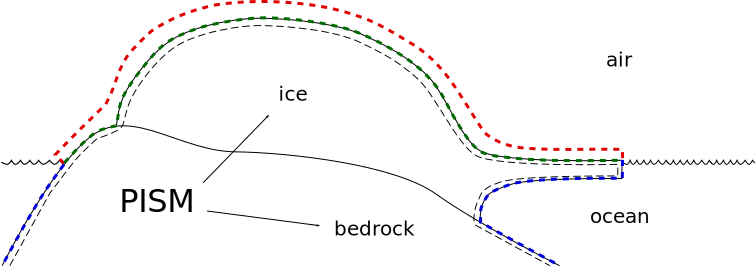
\includegraphics[width=6in]{figs/climate-cartoon.pdf}
  \caption{PISM's view of interfaces between an ice sheet and the outside world}
  \label{fig:climate-inputs}
\end{figure}

Because PISM's job is to approximate ice flow, its ``world view'' is centered around ice dynamics.  The discussion of boundary conditions in this Manual is thus ice-dynamics-centric.  On the other hand, there is no constraint on the nature of, or completeness of, climate models which could be coupled to PISM.  This section therefore explains a PISM organizing principle, namely that \emph{climate inputs affect ice dynamics by a well-defined interface}.

Almost no attempt is made here to describe the physics of the climate around ice sheets, so see \cite{massbalanceglossary} for terminology and \cite{Hock05} for a review of how surface melt can be modeled.  See the Climate Forcing Manual for much more information on PISM's climate-coupling-related options and on the particular fields which are shared between the ice dynamics core and the climate model.  Table \ref{tab:ice-dynamics-bc} lists fields which are needed as boundary conditions at the interfaces.

All PISM ice sheet models have some kind of interface (\textcolor{ForestGreen}{\textbf{green}} in Figure \ref{fig:climate-inputs}) to a subaerial surface processes layer containing snow, firn, and liquid (or refrozen) runoff.  The surface layer is assumed to cover the whole surface of the ice, and all grounded areas that the ice might occupy, including ablation areas and ice-free land.  We also always have an interface (\textcolor{blue}{\textbf{blue}}) to the ocean, but this interface is inactive if there is no floating ice.

\begin{table}[ht]
  \centering
 \begin{tabular}{p{0.45\linewidth}p{0.5\linewidth}}
    \toprule
    \textbf{Boundary surface} & \textbf{Fields (conditions)} \\
    \midrule
    upper surface of the surface processes layer (\textcolor{red}{\textbf{red}}) & \emph{optional}; typically: air temperature, precipitation \\
    top ice surface, but below firn (\textcolor{ForestGreen}{\textbf{green}}) & \emph{required}: boundary temperature (or enthalpy), mass flux (SMB) into the ice\\
    ice shelf basal surface (\textcolor{blue}{\textbf{blue}}) & \emph{required}: mass flux into the ocean, boundary temperature\\
    bottom surface of thermally-modeled bedrock layer (not shown) & \emph{required}: geothermal flux\\
   \bottomrule
  \end{tabular}
\caption{Boundary conditions required by PISM's ice dynamics core; see Figure \ref{fig:climate-inputs}.  The optional \textcolor{red}{\textbf{red}} interface is absent if PISM does not ``own'' the surface processes layer.}
\label{tab:ice-dynamics-bc}
\end{table}

The surface processes layer might be very simple.  It might either read the important fields from a file or otherwise transfer them from a separate (non-PISM) climate model.  If, however, the surface processes layer is ``owned'' by the PISM model then there is an additional interface (\textcolor{red}{\textbf{red}}) to the atmosphere above.  In no case does PISM ``own'' the atmosphere; if it has an interface to the atmosphere at all then it reads atmosphere fields from a file or otherwise transfers them from a climate model.

Regarding the base of the ice, the temperature of a layer of bedrock in contact with grounded ice is generally included in PISM's conservation of energy model; see subsections \ref{subsect:coords} and \ref{subsect:grid}.   Also, as described in section \ref{subsect:beddef}, PISM can apply an optional bed deformation component approximating the movement of the Earth's crust and upper mantle in response to changing ice load.  In these senses everything below the black dashed line in Figure \ref{fig:climate-inputs} is always ``owned'' by PISM.

The PISM ice dynamics core would like to get the required fields listed in Table
\ref{tab:ice-dynamics-bc} directly from observations or measurements, or directly from a GCM.  In many realistic modeling situations, however, PISM code must be used for all or part of the surface processes modeling necessary to provide the ice-dynamics core with the needed fields.  Due to differences in model resolutions and required down-scaling, this need for some PISM-based boundary-processes modelling may occur even in some cases where PISM is coupled to a GCM.  Thus, to be able to use the data that is available, a PISM run might use components that are responsible for modeling surface (snow) processes or sub-shelf/ocean interaction.  These components might be very minimal, merely turning data that we already have into data in the right units and with the right metadata.

\begin{figure}[ht]
  \centering
  \includegraphics[width=4.0in]{figs/data-flow.pdf}
  \caption{PISM climate input data flow. Colored arrows correspond to interfaces in
    Figure \ref{fig:climate-inputs}.}
  \label{fig:climate-input-data-flow}
\end{figure}

Thus we have PISM's design: the ice-dynamics PISM core does not contain any parameterization or other model for boundary mass or energy fluxes into or out of the ice.  These boundary parameterizations and models are present in the PISM source code, however, as instances of \emph{PISMComponent} classes.  This simplifies customizing and debugging PISM's climate inputs, and it promotes code reuse.  It isolates the code that needs to be changed to couple PISM to different climate models.

The classes \mbox{\emph{PISMSurfaceModel}}, \mbox{\emph{PISMAtmosphereModel}}, and \mbox{\emph{PISMOceanModel}} are all derived from \mbox{\emph{PISMComponent}}.  Corresponding to the \textcolor{red}{\textbf{red}} dashed line in Figure~\ref{fig:climate-inputs}, a \mbox{\emph{PISMAtmosphereModel}} might not even be present in some PISM configurations.  While they are required, \emph{PISMSurfaceModel} and \emph{PISMOceanModel} may contain (hide) anything from nearly-trivial parameterizations of ice surface temperatures and mass fluxes to a GCM of great complexity.  

The ``modifiers'' in Figure \ref{fig:climate-input-data-flow} adjust the
climate model inputs.  Modifiers can be chained together so that multiple modifications
are made to the outputs of the original component.  For example,
ice-core-derived air temperature offsets, used to model the space-time
distribution of paleo-climatic surface temperature, is an example of an
implemented modifier.  Please see the Climate Forcing Manual for
a list of climate components and modifiers included in PISM source code and other details.
Users wishing to customize PISM's climate inputs and/or couple PISM to a climate
model should additionally see the \emph{PISM Source Browser} at \url{\PISMBROWSERURL}
and the documentation therein.

Figure~\ref{fig:climate-input-data-flow} illustrates the data flow needed
by the ice dynamics core.  The data flow in the other direction, i.e.~needed by the
model to which PISM is coupled, depends on particular modeling choices, but
great flexibility is allowed.

Why describe all this structure here?  On the one hand, some users may be interested
in coupling PISM to other models.  On the other hand, the PISM authors do not
claim expertise in modeling atmosphere, ocean, or even snow processes.  This
separation has a definite code-reliability purpose.  PISM users
are ultimately responsible for providing the climate inputs they intend.


\clearpage\newpage

\section{Modeling choices: Grid and time}
\label{sec:modeling-computational}

\subsection{Computational box} \label{subsect:coords}
\optsection{Computational box}
\optseealso{Grid}

PISM does all simulations in a computational box\index{PISM!computational box} which is rectangular in the PISM coordinates.

The coordinate system has horizontal coordinates $x,y$ and a vertical coordinate $z$.  The $z$ coordinate is measured positive upward from the base of the ice and it is exactly opposite to the vector of gravity.  The surface $z=0$ is the base of the ice, however, and thus is usually not horizontal in the sense of being parallel to the geoid.   The surface $z=0$ is the base of the ice both when the ice is grounded and when the ice is floating.

Bed topography is, of course, allowed.  In fact, when the ice is grounded, the true physical vertical coordinate $z'$, namely the coordinate measure relative to a reference geoid, is given by $z'=z+b(x,y)$ where $b(x,y)$ is the bed topography.  The surface $z'=h(x,y)$ is the surface of the ice.

In the grounded case the equation $h(x,y)=H(x,y)+b(x,y)$ always applies if $H(x,y)$ is the thickness of the ice.  In the floating case, the physical vertical coordinate is $z'=z-(\rho_i/\rho_s) H(x,y)$ where $\rho_i$ is the density of ice and $\rho_s$ the density of sea water.  Again $z=0$ is the base of the ice, which is the surface $z' = -(\rho_i/\rho_s) H(x,y)$.  The surface of the ice is $h(x,y) = (1-\rho_i/\rho_s) H(x,y)$.  All we know about the bed elevations is that they are below the base of the ice when the ice is floating.  That is, the \emph{flotation criterion} $-(\rho_i/\rho_s) H(x,y) > b(x,y)$ applies.

The computational box can extend downward into the bedrock.  As $z=0$ is the base of the ice, the bedrock corresponds to negative $z$ values regardless of the sign of its true (i.e.~$z'$) elevation.

The extent of the computational box, along with its bedrock extension downward, is determined by four numbers \texttt{Lx}, \texttt{Ly}, \texttt{Lz}, and \texttt{Lbz} (see Figure \ref{fig:rectilinearbox}.).  The first two of these are half-widths and have units of kilometers when set by options or displayed.  The extent of the computational box for the ice and bedrock is directly controlled by the following options. 

\begin{center}
  \begin{tabular}{llp{0.7\linewidth}}
    \toprule
    \textbf{Option} & \textbf{Meaning}
    \\\midrule
    \txtopt{Lx}{(km)} & Half-width of the computational domain (in the $x$-direction) \\
    \txtopt{Ly}{(km)} & Half-width of the computational domain (in the $y$-direction) \\
    \txtopt{Lz}{(meters)} & Height of the computational domain in the ice \\
    \txtopt{Lbz}{(meters)} & Depth of the computational domain in the bedrock thermal layer
    \\\bottomrule
  \end{tabular}
\end{center}

\begin{figure}[ht]
\centering
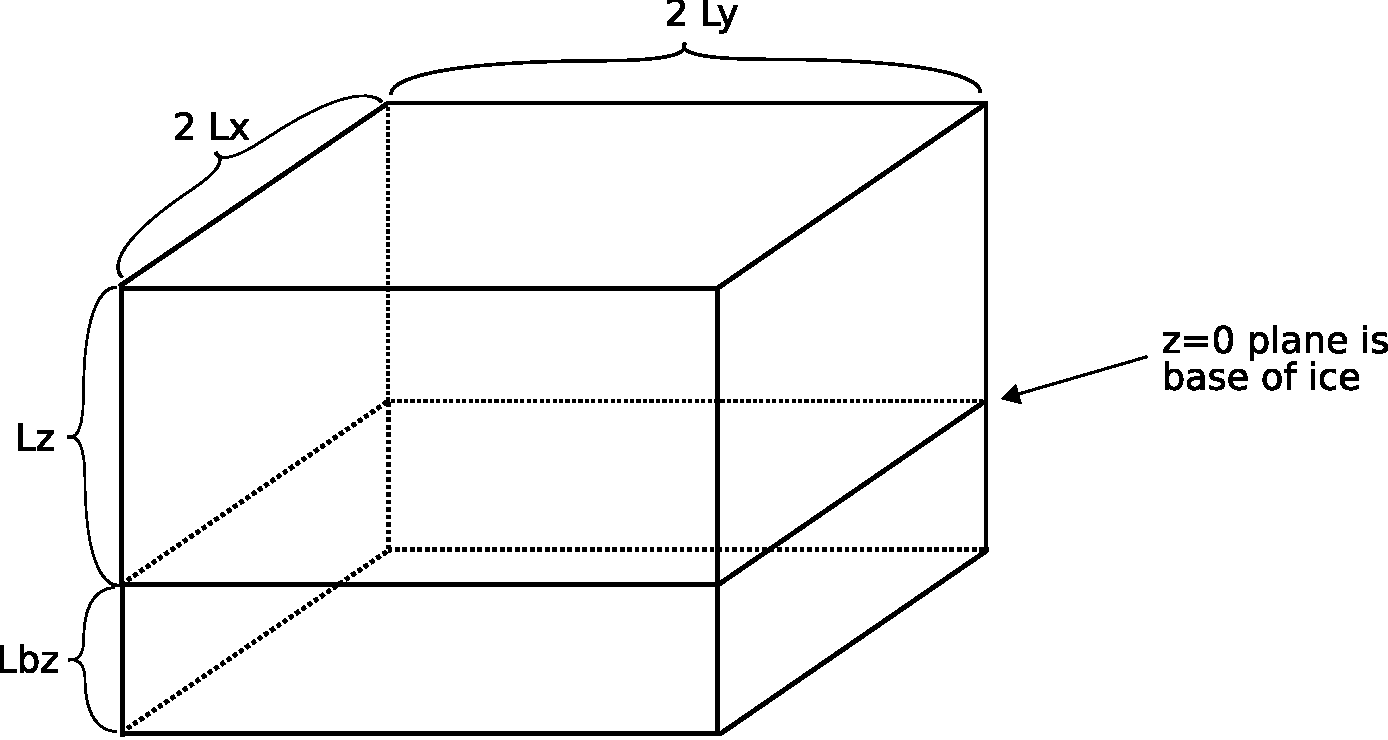
\includegraphics[width=4.0in,keepaspectratio=true]{rectilinearbox}
\caption{PISM's computational box.}
\label{fig:rectilinearbox}
\end{figure}


\subsection{Spatial grid}
\label{subsect:grid}
\optsection{Grid!space}

The PISM grid\index{PISM!grid} covering the computational box is equally spaced in horizontal ($x$ and $y$) directions.  Vertical spacing in the ice is quadratic by default (see below) but optionally a different spacing scheme can be chosen.  (Choose with options \txtopt{z_spacing}{[quadratic, equal]}.) The bedrock thermal layer model always uses equal vertical spacing.

The grid is described by four numbers, namely the number of grid points \texttt{Mx} in the $x$ direction, the number \texttt{My} in the $y$ direction, the number \texttt{Mz} in the $z$ direction within the ice, and the number \texttt{Mbz} in the $z$ direction within the bedrock thermal layer.  These are specified by options \intextoption{Mx}, \intextoption{My}, \intextoption{Mz}, and \intextoption{Mbz}, respectively. The defaults are 61, 61, 31, and 1, respectively.

Note that \texttt{Mx}, \texttt{My}, \texttt{Mz}, and \texttt{Mbz} all indicate the number of grid \emph{points}.  The numbers of grid \emph{spaces} are one less, thus 60, 60, 30, and 0 in the default case.  The lowest grid point in a column of ice, at $z=0$, coincides with the highest grid point in the bedrock, so \texttt{Mbz} must always be at least one and \texttt{Mbz}$>1$ is required to use the bedrock thermal model.  Note that this option is unrelated to the bed deformation model (glacial isostasy model); see option \texttt{-bed_def} (section \ref{subsect:beddef}) for that.

In the quadratic case, the spacing near the ice/bedrock interface is about four times finer than it would be with equal spacing for the same value of \texttt{Mz}, while the spacing near the top is correspondingly coarser. For a detailed description of the spacing of the grid, see the documentation on \texttt{IceGrid::compute_vertical_levels()} in the PISM class browser.

When a thermal bedrock layer is used, the distance \texttt{Lbz} is controlled by the \texttt{-Lbz} option.

If one initializes PISM from a saved model state using \texttt{-i} then the input model state controls all computational grid parameters.  For instance, the command

\begin{verbatim}
$  pismr -i foo.nc -y 100
\end{verbatim}

\noindent should work fine if \texttt{foo.nc} was a valid PISM model file.  The command

\begin{verbatim}
$  pismr -i foo.nc -Mz 201 -y 100
\end{verbatim}

\noindent will give a warning that ``\texttt{PISM WARNING: ignoring command-line option '-Mz'}'' because \texttt{-i} input files take precedence.

Otherwise, one is allowed to specify the grid when PISM is started.  In particular, the user should specify the grid when using \texttt{-boot_file} or when initializing a simplified-geometry experiment or a verification test, though defaults are generally present in the latter cases.  See sections \ref{sec:start} and \ref{sec:boot} for examples and explanation.


\subsection{Model time}
\label{sec:time}
\optsection{Grid!time}

The following command-line options control PISM time:

\begin{tabular}{lp{0.8\linewidth}}\\
\toprule
\textbf{Option} & \textbf{Meaning}\\
\midrule
\txtopt{y}{(years)} & Number of model years to run.\\
\txtopt{ys}{(years)} & Model year at which to start the run.  Also resets the model time, ignoring any time in the input file.\\
\txtopt{ye}{(years)} & Model year at which to end the run.\\
\bottomrule
\end{tabular}
\\[2em]
\noindent The default value for the end year is the start year (\texttt{-ys} or initialized model time from file) plus the default or given (\texttt{-y}) run length.  If both \texttt{-ys} and \texttt{-ye} are used then the run length is set to the difference.  Using all three of \texttt{-ys}, \texttt{-y} and \texttt{-ys} is not allowed.


\subsection{Calendars}
\label{sec:calendars}
\index{Time!calendars}

Most of PISM (and its ice dynamics core in particular) only needs to know the length of the current time-step.  Internally PISM stores time in ``seconds since a specified moment'' and thus PISM generally does not use or need a calendar.\footnote{Note seconds are part of SI units.}  We refer to PISM internal time as \emph{model time}.

One can select a calendar for a more precise control of the model time, however.  Choosing a calendar is appropriate for runs for specific temporal periods like ``the 18th-century'' or ``1989--2010''.  The calendar is generally needed because  specific knowledge of lengths of months and years is required to use climate data properly and to facilitate model validation.  A ``calendar'' is a concept that is part of the \href{http://cf-pcmdi.llnl.gov/documents/cf-conventions/1.6/cf-conventions.html}{CF Metadata Conventions}.

You can choose a calendar by setting the \config{calendar} configuration
parameter or the command-line options described below in Table \ref{tab:calendars}.

\begin{table}
  \centering
  \begin{tabular}{lp{0.7\linewidth}}
    \texttt{gregorian} or \texttt{standard} & Mixed Gregorian/Julian calendar used today.\\
    \texttt{proleptic_gregorian} & Gregorian calendar extended to dates before 1582-10-15.\\
    \texttt{noleap} or \texttt{365_day} & Calendar with fixed-length 365-day years\\
    \texttt{360_day} & Calendar with fixed-length 360-day years divided into 30-day months\\
    \texttt{julian} & Julian calendar \\
    \texttt{none} & no calendar\\
  \end{tabular}
  \caption{Calendars supported by PISM. Please see \href{http://meteora.ucsd.edu/~pierce/calcalcs/calendars.html}{CalCalcs documentation} for details.}
  \label{tab:calendars}
\end{table}

PISM uses
\href{http://meteora.ucsd.edu/~pierce/calcalcs/index.html}{CalCalcs}
by David~W.~Pierce to perform calendric computations. This lets us
support all the calendars
\href{http://cf-pcmdi.llnl.gov/documents/cf-conventions/1.6/cf-conventions.html#calendar}{defined}
by the CF Metadata Conventions document except for the
\texttt{366_day} (\texttt{all_leap}) calendar.

Time units in PISM's output files always contain a reference date
because it is required by the CF metadata conventions.

By default PISM does not use a calendar. This is appropriate for runs that
do not require precise application of forcing data or reporting on
particular dates (paleo-climate runs, for example).
In this mode PISM ignores the reference date in time unit specifications
(such as ``\texttt{days since 1969-7-20}''), though the value set using
\config{reference_date} configuration parameter is saved in
output files.

Selecting a calendar using the \config{calendar} configuration
parameter or the \intextoption{-calendar} command-line option enables calendar-based time management.

The implications are:
\begin{itemize}
\item PISM uses the \texttt{units} attribute of coordinate variables
  \emph{literally} (including the reference date) in unit conversions. Please
  make sure that the \variable{time} variable in all forcing files has the
  units attribute such as ``\texttt{days since 2012-1-1}''. PISM will stop with
  an error message if a time variable does not have a reference date in its
  unit specification.
\item It is important to use units that are a fixed multiple of ``seconds'',
  such as ``\texttt{minutes since 1989-1-1}'' or ``\texttt{days since
    1999-12-31}'' and avoid ``months'' and ``years''. (PISM uses UDUNITS-2 to
  convert units, and in UDUNITS one month is always interpreted as
  $\frac{1}{12}\cdot 365.242198781$ days.) Please see the 
  \href{http://cf-pcmdi.llnl.gov/documents/cf-conventions/1.6/cf-conventions.html#time-coordinate}{CF
    Conventions} document for details.
\item PISM uses dates in standard output:
\begin{verbatim}
...
   time interval (length)   [2012-01-01, 2021-12-31]  (10.000 years)
...
S 2012-05-26:  0.00011    0.6306   0.00000000           0.00000
$v$Eh m (dt=0.10000)
S 2012-07-01:  0.00014    0.6306   0.00000000           0.00000
\end{verbatim}
\end{itemize}

Just like in the no-calendar mode, run length, run start and run end
times are specified using \intextoption{y}, \intextoption{ys} and
\intextoption{ye} command-line options, respectively. Arguments of
these options are interpreted in a slightly different manner, though:
\begin{itemize}
\item the run length option \texttt{-y} takes an \emph{integer}
  argument, interpreted as the number of \emph{calendar} years
\item options \texttt{-ys} and \texttt{-ye} take \emph{dates} as arguments.
\end{itemize}

For example, either of the following commands sets up a run covering the 21$^{st}$ century:
\begin{verbatim}
$ pismr -calendar gregorian -ys 2001-1-1 -y 100 ...
$ pismr -calendar standard -ys 2001-1-1 -ye 2101-1-1 ...
\end{verbatim}
(These option combinations are equivalent.)

It is also possible to run PISM for the duration of the available forcing data using the \fileopt{time_file} option.
This command
\begin{verbatim}
$ pismr -calendar gregorian -time_file forcing.nc
\end{verbatim} %$
will extract the reference date and run length from \texttt{forcing.nc}, respecting time bounds.

It is also possible to save spatial and/or scalar time-series daily, monthly or
yearly (using the calendric computations). See sections~\ref{sec:saving-time-series}
and~\ref{sec:saving-spat-vari}.

\subsection{Diagnostic computations}
\label{sec:diagnostic-computations}

A diagnostic computation is one where the internal state does not evolve.  The major way this can happen is if the run duration is zero years.  Such runs are often used to look at lots of fields for the current model state.

As an example, consider the second of these two runs:
\begin{verbatim}
pisms -y 6000 -o foo.nc
pismr -i foo.nc -y 0 -o bar.nc -o_size big
\end{verbatim}

\noindent The result of this zero-length, ``\texttt{-y 0}'', run is a NetCDF file \texttt{bar.nc} which contains the full three-dimensional velocity field in the scalar NetCDF variables \texttt{uvel}, \texttt{vvel}, and \texttt{wvel}, as well as many other variables.  The file \texttt{foo.nc} does not contain many of these fields because it was written with the default output size of \texttt{medium}.  The ``\texttt{-y 0}'' run has diagnostically ``filled-in'' all the fields which PISM can model at a time step, but the model state has not evolved.

In fact, during such a run PISM performs one short time-step to compute ``rates of change'' of ice thickness, surface elevation and other fields, but the model state \emph{is reset} after this step, so re-starting from \texttt{foo.nc} above would give the same result as re-starting from \texttt{bar.nc}.

This diagnostic mode is often associated to the modeling of ice shelves and ice streams.  Subsection \ref{sec:ross} describes using a ``\texttt{-y 0}'' diagnostic run to model the Ross ice shelf \cite{MacAyealetal}.  Verification tests I and J, section \ref{sec:verif}, are diagnostic calculations using the SSA.

Note that the NetCDF model state saved by PISM at the end of an \emph{evolution} run does not, under the default \texttt{-o_size medium} output size, contain the three-dimensional velocity field.  Instead, it contains just a bit more than the variables which are needed to restart the run.  One can  force PISM to save all the supported diagnostic quantities at the end of a time-stepping run using the option \texttt{-o_size big}.  Or one can go back and do a ``\texttt{-y 0}'' diagnostic run and ask for \texttt{-o_size big}.


\subsection{Disabling PISM components}
\label{sec:turning-off}
\optsection{Disabling PISM components}

Certain major model components, unlike more peripheral ones like bed deformation or calving, are ``on'' by default.  They do not need to be turned on explicitly.  For example, the SIA computation is so common that it would be a hassle to require an option to turn it on every time you need it.

But sometimes one wants to disable particular components, during model spin-up, for example.  PISM has the following ``off'' switches:
\begin{itemize}
\item \intextoption{no_mass} disables the mass-continuity (conservation of mass) step
\item \intextoption{no_energy} disables the conservation of energy computation
\item \intextoption{cold} makes PISM use temperature instead of enthalpy in the energy conservation code
\item \intextoption{no_sia} disables the SIA stress balance computation (useful for ice-shelf modeling)
\end{itemize}


\subsection{Dealing with more difficult modeling choices}
\label{subsec:hard-choices}\optsection{Dealing with more difficult modeling choices}

Most uses of an ice sheet model depend on careful modeling choices in situations where there are considerable uncertainties \emph{and} the model results depend strongly on those choices.  There may be, at the present state of knowledge, \emph{no clear default values} that PISM can provide.  Also, the available PISM options and sub-models are known to \emph{not} be sufficient for all users.  Thus there are modeling choices for which we know the user may have to do a great deal more hard work than just choose among PISM runtime options.

Here are example cases where users have worked hard:
\begin{itemize}
\item User made use of available data in order to choose parameters for existing PISM models.  These parameters will then override PISM defaults.
\begin{center} % our UAF current situation with Greenland
\fbox{ \begin{minipage}[t]{5.0in}
\emph{Example}.  Use regional atmosphere model output to identify PDD parameters suitable for modeling surface mass balance on a particular ice sheet.  Then supply these parameters to PISM by a \texttt{-config\_override} file.
\end{minipage} }
\end{center}
\item User wrote code, including code which modified current PISM internals, either to add additional processes or to ``correct'' PISM default process models.
\begin{center} % the ocean coupler-related Potsdam marine ice sheet mods
\fbox{ \begin{minipage}[t]{5.0in}
\emph{Example}.  Add a new sub-ice-shelf melt model by modifying C++ code in the \texttt{src/coupler/} directory.
\end{minipage} }
\end{center}
\item User simplified the model in use, instead of the default which was more elaborate.
\begin{center} % Nick's -yield_stress constant choice
\fbox{ \begin{minipage}[t]{5.0in}
\emph{Example}.  Instead of using the PISM default mechanism connecting basal melt rate and basal strength, bypass this mechanism and impose a map of yield stress \texttt{tauc} directly.
\end{minipage} }
\end{center}
\end{itemize}


%%% Local Variables: 
%%% mode: latex
%%% TeX-master: "manual"
%%% End: 

% LocalWords:  


\clearpage\newpage

\section{Modeling choices:  Ice dynamics and the subglacier}
\label{sec:modeling-dynamics}

\subsection{Ice rheology}
\label{sec:rheology}
\optsection{Ice rheology}

The ``rheology'' of a viscous fluid refers to the relation between the applied stress and the resulting deformation, specifically the strain rate.  The models of ice rheology available in PISM are of isotropic Glen-Nye type \cite{Paterson}.   A rheology in this class is described by a ``flow law'', which is a function $F(\sigma,T,\omega,P,d)$ in the ``constitutive relation''
\begin{equation}
D_{ij} = F(\sigma,T,\omega,P,d)\, \sigma_{ij}'.  \label{eq:constitutive}
\end{equation}
Here $D_{ij}$ is the strain rate tensor, $\sigma_{ij}'$ is the stress deviator tensor, $T$ is the ice temperature, $\omega$ is the liquid water fraction, $P$ is the pressure, and $d$ is the grain size.  Also $\sigma^2 = \frac{1}{2} \|\sigma_{ij}'\|_F = \frac{1}{2} \sigma_{ij}' \sigma_{ij}'$; $\sigma$ is the second invariant of the stress deviator tensor.

For example,
\begin{equation}
F(\sigma,T) = A(T) \sigma^{n-1}  \label{eq:isothermalglen}
\end{equation}
is the common temperature-dependent Glen law \cite{PatersonBudd,BBL}, which has no dependence on liquid water fraction, pressure, or grain size.  If the ice softness $A(T)=A_0$ is constant then the law is isothermal, whereas if there is dependence on temperature then $A(T)$ is most-commonly a generalization of ``Arrhenius'' form $A(T) = A \exp(-Q/RT^*)$.  The more elaborate Goldsby-Kohlstedt law \cite{GoldsbyKohlstedt} is a function $F(\sigma,T,P,d)$.

In the enthalpy mode of PISM, which is the thermodynamical modeling default, there is only one choice for the flow law: the Glen-Paterson-Budd-Lliboutry-Duval law \cite{AschwandenBuelerKhroulevBlatter,LliboutryDuval1985,PatersonBudd}, a function $F(\sigma,T,\omega,P)$.  This law is the only one in the literature that depends on both the temperature and the liquid water fraction; it parameterizes the (observed) softening of pressure-melting-temperature ice as its liquid fraction increases.  One can use this polythermal law or one may choose among a number of ``cold ice'' laws listed in Table \ref{tab:flowlaw} which do not use the liquid water fraction.  

Command-line options \intextoption{sia_flow_law} and \intextoption{ssa_flow_law} control which flow law is used by the SIA and SSA ice dynamics models.  Allowed arguments are listed in table \ref{tab:flowlaw} below.  Form \eqref{eq:constitutive} of the flow law is used in the SIA.  However, the ``viscosity'' form of such a flow law, found by inverting the constitutive relation, is needed for ice shelf and ice stream (SSA) flow \cite{BBssasliding}:
	$$\sigma_{ij}' = 2 \nu(D,T,\omega,P,d)\,D_{ij} $$
Here $\nu(D,T,\omega,P,d)$ is the ``effective viscosity'' and $D^2 = \frac{1}{2} D_{ij} D_{ij}$.  Viscosity form is not known for the Goldsby-Kohlstedt law \cite{GoldsbyKohlstedt}, so option ``\texttt{-ssa_flow_law gk}'' is an error.

One can also choose either \texttt{-sia_flow_law isothermal_glen} or \texttt{-ssa_flow_law isothermal_glen}, which is $F(\sigma) = A_0 \sigma^{n-1}$ and its inverse $\nu(D) = \frac{1}{2} B_0 D^{(1-n)/(2n)}$, respectively, where $A_0$ is the isothermal ice softness and $B_0=A_0^{-1/n}$ is the isothermal ice hardness.

The command-line options \intextoption{sia_e} and \intextoption{ssa_e} set flow enhancement factors for the SIA and SSA respectively. These options can be used with any flow law.  Option \texttt{-sia_e} sets ``$e$'' in ``$D_{ij} = e\, F(\sigma,T,\omega,P,d)\, \sigma_{ij}',$'' in equation \eqref{eq:constitutive}.  Option \texttt{-ssa_e} sets ``$e$'' in the viscosity form so that ``$\sigma_{ij}'  = e^{-1/n}\, 2\, \nu(D,T,\omega,P,d)\, D_{ij}.$''

Flow law parameters such as ice softness can be changed using configuration parameters (see section \ref{sec:pism-defaults} and the implementation of flow laws in the \emph{Source Code Browser}).  One can also choose the scalar function $F$ reasonably arbitrarily by modifying source code; see source files \texttt{flowlaws.hh}, \texttt{flowlaws.cc} in \texttt{src/base/rheology/}.  Table \ref{tab:flowlaw} therefore also lists the C++ classes declared in \texttt{flowlaw.hh}.

\begin{table}[ht]
\centering
\index{rheology}\index{flow law}
\small
\begin{tabular}{p{0.18\linewidth}p{0.2\linewidth}p{0.52\linewidth}}\toprule
\textbf{Type} & C++ Class & \textbf{Comments and Reference} \\ \midrule
\texttt{pb} &\texttt{ThermoGlenIce}  & Paterson-Budd law, the cold-mode default.  Fixed Glen exponent $n=3$.  There is a split ``Arrhenius'' term $A(T) = A \exp(-Q/RT^*)$ where \mbox{$A = 3.615 \times 10^{-13}\, \text{s}^{-1}\, \text{Pa}^{-3}$}, \mbox{$Q = 6.0 \times 10^4\, \text{J}\, \text{mol}^{-1}$} if $T^* < 263$ K and
 \mbox{$A = 1.733 \times 10^{3}\, \text{s}^{-1}\, \text{Pa}^{-3}$}, \mbox{$Q = 13.9 \times 10^4\, \text{J}\, \text{mol}^{-1}$} if $T^* > 263$ K and where $T^*$ is the pressure-adjusted temperature \cite{PatersonBudd}. \\
\texttt{arr} &  \texttt{ThermoGlenArrIce} & \emph{Cold} part of Paterson-Budd.  Regardless of temperature, the $A$ and $Q$ values for $T^*<263$ K in  the Paterson-Budd law apply.  This is the flow law used in the thermomechanically coupled exact solutions Tests \textbf{F} and \textbf{G} described in \cite{BBL,BB} and run by \texttt{pismv -test F} and \texttt{pismv -test G}. \\
\texttt{arrwarm} & \texttt{ThermoGlenArrIceWarm} & \emph{Warm} part of Paterson-Budd.  Regardless of temperature, the $A$ and $Q$ values for $T^*>263$ K in Paterson-Budd apply.\\
\texttt{hooke} & \texttt{HookeIce} & Hooke law.  Fixed Glen exponent $n=3$.  Here  \mbox{$A(T) = A \exp(-Q/(RT^*) + 3C (T_r - T^*)^\kappa)$;} values of  constants as in \cite{Hooke,PayneBaldwin}.\\
\texttt{gk} & \texttt{GoldsbyKohlstedtIce} & The  Goldsby-Kohlstedt flow law.  This law has a combination of exponents  from $n=1.8$ to $n=4$ \cite{GoldsbyKohlstedt}. It does not have a viscosity form and can only be used by the SIA stress balance. \\
\texttt{isothermal_glen} &  \texttt{IsothermalGlenIce} &The isothermal Glen flow law. \\
\bottomrule
\normalsize	
\end{tabular}
\caption{Choosing the ice rheology using \texttt{-sia_flow_law} and \texttt{-ssa_flow_law}.  These flow law choices do not use the liquid water fraction.}
\label{tab:flowlaw}
\end{table}


\subsection{Choosing the stress balance}  \label{subsect:ssacontrol}
\optsection{SSA as a sliding law}

The basic stress balance used for all grounded ice in PISM is the non-sliding, thermomechanically-coupled SIA \cite{BBL}.  For the vast majority of most ice sheets, as measured by area or volume, this is an appropriate model which is an $O(\eps^2)$ approximation to the Stokes model \cite{Fowler}.

The shallow shelf approximation (SSA)\index{SSA (shallow shelf approximation)} stress balance applies to floating ice.  Option \texttt{-ssa_floating_only} turns on this stress balance but restricted only to floating ice.  See the Ross ice shelf example in section \ref{sec:ross} for an example in which the SSA is only applied to floating ice.

The SSA is also used in PISM to describe the sliding of grounded ice and the formation of ice streams \cite{BBssasliding}.  Specifically for the SSA with ``plastic'' (Coulomb friction) basal resistance, the locations of ice streams are determined as part of a free boundary problem of Schoof \cite{SchoofStream}, a model for emergent ice streams within a ice sheet and ice shelf system.  This model explains ice streams through a combination of plastic till failure and SSA stress balance.  As a combination of SIA and SSA it is a ``hybrid'' approximation of the Stokes model \cite{BBssasliding,Winkelmannetal2011}.  In other words, this SSA description of ice streams is the preferred ``sliding law'' for the SIA, and it should be used in preference to classical SIA sliding laws which make ice basal velocity a local function of the basal value of the driving stress \cite{BBssasliding}.\index{SIA (shallow ice approximation)!sliding laws}

Option \texttt{-ssa_sliding} turns on such use of the plastic till SSA as a sliding law; floating ice is also subject to the SSA with this option.  Of course the is more to the use of a stress balance than just turning it on.  At all grounded points a yield stress, or a pseudo-yield-stress in the case of power law sliding (subsection \ref{subsect:basestrength}), is computed from the amount of stored basal water and from a (generally) spatially-varying till strength.  The amount of stored basal water is modeled by the subglacial hydrology mode choice (subsection \ref{subsect:subhydro}) based on the basal melt rate which is, primarily, thermodynamically-determined (subsection \ref{subsect:basestrength}).

Table \ref{tab:stressbalchoice} describes the basic choice of stress balance, while Table \ref{tab:ssausage} describes additional controls on the numerical solution of the stress balance equations.  If the ice sheet being modeled has any floating ice then the user is advised to read section \ref{sec:pism-pik} on modeling marine ice sheets.

\begin{table}[ht]
\centering
\small
\begin{tabular}{p{0.25\linewidth}p{0.65\linewidth}}
\toprule
\textbf{Option} & \textbf{Semantics}\\ \midrule
    (\emph{NO OPTION}) & Grounded ice flows by the non-sliding SIA.  Floating ice essentially doesn't flow, so this model is not recommended for marine ice sheets. \\
    \intextoption{no_sia} & Do not use the SIA model anywhere. \\
    \intextoption{ssa_floating_only} & Only floating ice uses SSA.  Grounded ice marked by mask value \texttt{SHEET} uses the nonsliding SIA. \\
    \intextoption{ssa_sliding} & The recommended default sliding law, which gives the SIA+SSA hybrid stress balance.  Combines SSA-computed velocity, using pseudo-plastic till, with SIA-computed velocity according to the combination in \cite{BBssasliding}.  Floating ice uses SSA only. \\
\bottomrule
\end{tabular}
\normalsize
\caption{The basic choice of stress balance.}
\label{tab:stressbalchoice} 
\end{table}


\begin{table}
  \centering
  \begin{tabular}{p{0.22\linewidth}p{0.75\linewidth}}
     \toprule
     \textbf{Option} & \textbf{Description}\\\midrule
     \intextoption{ssa_method} [\texttt{fd}$\big|$\texttt{fem}] & Both finite difference (\texttt{fd}) and finite element (\texttt{fem}) versions of the SSA numerical solver are implemented in PISM.  They behave similarly for runs without PIK options (section \ref{sec:pism-pik}), but the \texttt{fd} solver is the only one which allows PIK options.  \texttt{fd} uses Picard iteration \cite{BBssasliding}, while \texttt{fem} uses a Newton method.  The \texttt{fem} solver has in-development surface velocity inversion capability \cite{Habermannetal2012}.  \\
     \intextoption{ssa_eps} (1.0e13) & The numerical scheme for the SSA computes an effective viscosity $\nu$ which which depends on strain rates and ice hardness (thus on temperature).  The value of, and the minimum of, the effective viscosity times the thickess (i.e.~$\nu H$) is important to ease of solving the numerical SSA.  This constant is added ($\nu H \to \nu H + \text{\texttt{ssa_eps}}$) to keep this quantity bounded away from zero.  The units of \texttt{ssa_eps} are $\text{Pa}\,\text{m}\,\text{s}$.  Turn off this lower bound mechanism by \texttt{-ssa_eps 0.0}.  Use option \texttt{-ssa_view_nuh} to view the product $\nu H$ for your simulation, to evaluate the relative importance of this \texttt{ssa_eps} regularization.  Note that a typical Greenland run might see a wide range of values for $\nu H$ from $\sim 10^{14}$ to $\sim 10^{20}$ $\text{Pa}\,\text{m}\,\text{s}$ for $\nu H$. \\
     \intextoption{ssa_maxi} (300) & (\emph{Only active with} \texttt{-ssa_method fd}, \emph{the default}.)  Set the maximum allowed number of Picard (nonlinear) iterations in solving the shallow shelf approximation.\\
     \intextoption{ssa_rtol} (1.0e-4) & (\emph{Only active with} \texttt{-ssa_method fd}, \emph{the default}.)  The numerical scheme for the SSA does a nonlinear iteration wherein velocities (and temperatures) are used to compute a vertically-averaged effective viscosity which is used to solve the equations for horizontal velocity.  Then the new velocities are used to recompute an effective viscosity, and so on.  This option sets the relative change tolerance for the effective viscosity.
In particular, the nonlinear part of the iteration requires that successive values $\nu^{(k)}$ of the vertically-averaged effective viscosity satisfy
	$\|(\nu^{(k)} - \nu^{(k-1)}) H\|_1 \le \text{\texttt{ssa_rtol}} \|\nu^{(k)} H\|_1$
in order to end the iteration with $\nu = \nu^{(k)}$.  (See also PETSc option \texttt{-ksp_rtol} to control relative tolerance for the iteration inside the linear solver.)\\
\bottomrule
\end{tabular}
\caption{Controlling the numerical SSA stress balance in PISM}
\label{tab:ssausage}
\end{table}


\subsection{Surface gradient method}
\label{subsect:gradient}
\optsection{Driving stress computation}

PISM computes surface gradients to determine the ``driving stress''
	$$(\tau_{d,x},\tau_{d,y}) = - \rho g H \grad h,$$
where $H$ is the ice thickness, and $h = H+b$ is the ice surface elevation.  The driving stress enters into both the SIA and SSA stress balances, but in the former the driving stress is needed on a staggered grid, while in the latter the driving stress is needed on the regular grid.

Surface gradients are computed by finite differences in several slightly-different ways.  There are options for choosing which method to use, but to the best of our knowledge there is no theoretical advice on the best, most robust mechanism.  There are three \intextoption{gradient} methods in PISM:

\noindent\texttt{-gradient mahaffy}\quad  This most ``standard'' way computes the surface slope onto the staggered grid for the SIA \cite{Mahaffy}.  It makes $O(\Delta x^2,\Delta y^2)$ errors.  For computations of driving stress on the regular grid, centered differencing is used instead.

\noindent\texttt{-gradient haseloff}\quad  This is the default method, but it only differs from the Mahaffy method at ice-margin locations.  It alters the \texttt{mahaffy} formula for the slope in those cases where an adjacent ice-free bedrock surface elevation is above the ice elevation.

\noindent\texttt{-gradient eta}\quad  In this method we first transform the thickness $H$ by $\eta = H^{(2n+2)/n}$ and then differentiate the sum of the thickness and the bed using centered differences:
	$$\grad h = \grad H + \grad b = \frac{n}{(2n+2)} \eta^{(-n-2)/(2n+2)} \nabla \eta + \nabla b.$$
Here $b$ is the bed elevation and $h$ is the surface elevation.  This transformation sometimes has the benefits that the surface values of the horizontal velocity and vertical velocity, and the driving stress, are better behaved near the margin.  See \cite{BLKCB,CDDSV} for technical explanation of this transformation and compare \cite{SaitoMargin}.  The actual finite difference schemes applied to compute the surface slope are similar to option \texttt{mahaffy}.


\subsection{Parameterization of bed roughness in the SIA} \label{subsect:bedsmooth} \index{Parameterization of bed roughness}
\optsection{Parameterization of bed roughness}

Schoof \cite{Schoofbasaltopg2003} describes how to alter the SIA stress balance to model ice flow over significant subglacial bedrock topgraphy.  One uses a smoothed (spatially-averaged) bed, but one also lowers the SIA diffusivity, in a precise way, related to how much the topography was smoothed-away.  As a practical matter for PISM, this theory improves the SIA's ability to handle bed roughness because it parameterizes the effects of "higher-order" stresses which act on the ice as it flows over bed topography.  There is also a mild performance boost because of the reduction of diffusivity.  For additional technical description of PISM's implementation, see the \emph{Browser} page ``Using Schoof's (2003) parameterized bed roughness technique in PISM''.

There is only one associated option: \intextoption{bed_smoother_range} gives the half-width of the square smoothing domain in meters.  If zero is given, \texttt{-bed_smoother_range 0} then the mechanism is turned off.  The mechanism is on by default using executable \texttt{pismr}, with the half-width set to 5 km (\texttt{-bed_smoother_range 5.0e3}), giving the recommended smoothing size of 10 km \cite{Schoofbasaltopg2003}.  This mechanism is turned off by default in executables \texttt{pisms} and \texttt{pismv}.

PISM writes fields \texttt{topgsmooth}, \texttt{schoofs_theta}, \texttt{thksmooth} from this mechanism.  (Regarding the last, the thickness is never actually smoothed.  However, the thickness relative to the smoothed bedrock elevation, i.e.~the difference between the unsmoothed surface elevation and the smoothed bedrock elevation, is used internally in the mechanism.)


\subsection{Controlling basal strength}  \label{subsect:basestrength}
\optsection{Basal strength and sliding}

When using option \texttt{-ssa_sliding}, the SIA+SSA hybrid model, a sub-model for basal resistance is required.  That is, a \emph{sliding law} must be chosen.  Table \ref{tab:basal-strength} describes the options that control how basal resistance is computed.

\begin{table}
  \centering
 \begin{tabular}{lp{0.6\linewidth}}
    \\\toprule
    \textbf{Option} & \textbf{Description}
    \\\midrule
    \intextoption{hold_tauc} &   Keep the current values of the till yield stress $\tau_c$.  That is, do not update them by the default model using the stored basal melt water.  Only effective if \texttt{-ssa_sliding} is also set.  Normally used in combination with \texttt{-tauc}. \\
    \intextoption{pseudo_plastic} & enables the pseudo-plastic till model \\
    \intextoption{plastic_c0} & Set the value of the till cohesion ($c_{0}$) in the plastic till model.  The value is a pressure, given in kPa.\\
    \txtopt{plastic_reg}{(m/a)} & Set the value of $\eps$ regularization of plastic till; this is the second ``$\eps$'' in formula (4.1) in \cite{SchoofStream}. The default is $0.01$.\\
    \txtopt{plastic_phi}{(degrees)} & Use a constant till friction angle. The default is $30^{\circ}$.\\
    \intextoption{pseudo_plastic_q} & Set the exponent $q$.\\
    \txtopt{pseudo_plastic_uthreshold}{(m/a)} & Set $u_{\text{threshold}}$. The default is $100$ m/a.\\
    \txtopt{topg_to_phi}{\emph{list of 4 numbers}} & Compute $\phi$ using equation \eqref{eq:2}.\\
    \intextoption{tauc} &   Directly set the till yield stress $\tau_c$ in units of Pa.  Only effective if used with \texttt{-hold_tauc}, because otherwise $\tau_c$ is updated dynamically.
   \\ \bottomrule
  \end{tabular}
\caption{Basal strength command-line options}
\label{tab:basal-strength}
\end{table}

In PISM the strength value is always a basal yield stress $\tau_c$ (=\verb|tauc| in PISM output files).  This parameter represents the strength of the aggregate material at the base of an ice sheet, a poorly-observed mixture of liquid water, ice, granular till, and bedrock bumps.  The yield stress concept also extends to the power law form, and thus most standard sliding laws can be chosen by user options (below).

One reason that the yield stress is a useful parameter is that it can be compared, when looking at PISM output files, to the driving stress.  Specifically, where \verb|tauc| $<$ \verb|taud_mag| you are likely to see sliding if option \verb|ssa_sliding| is used.

The value of $\tau_c$ is determined in part by a subglacial hydrology model, including the modeled till-pore water pressure \verb|tillwat| (subsection \ref{subsect:subhydro}).  The value of $\tau_c$ is also determined in part by a stored basal material property $\phi=$\texttt{tillphi}, the ``till friction angle'' \cite{Paterson}.  These quantities combine in the Mohr-Coulomb criterion \cite[Chapter 8]{Paterson} to determine the basal yield stress:
\begin{equation}
   \tau_c = c_{0} + (\tan\phi)\,N_{til}.  \label{eq:mohrcoulomb}
\end{equation}
Here $c_0$ is called the ``till cohesion'', whose default value in PISM is zero \cite[formula (2.4)]{SchoofStream}.

The effective pressure on the till $N_{til}$ is a modeled quantity determined by assuming a compressible saturated till.  In this compressible-till model the till effective pressure $N_{til}$ is a locally-computable function of the amount of water in the till $W_{til} =$ \verb|tillwat| \cite{BuelervanPeltDRAFT}:
\begin{equation}
N_{til} = \delta P_o \, 10^{(e_0/C_c) \left(1 - (W_{til}/W_{til}^{max})\right)}  \label{eq:computeNtil}
\end{equation}
The following options control this local model:\begin{itemize}
\item \verb|-till_reference_void_ratio|$= e_0$, dimensionless, with default value 0.69 \cite{Tulaczyketal2000b},
\item \verb|-till_compressibility_coefficient| $= C_c$, dimensionless, with default value 0.12 \cite{Tulaczyketal2000b},
\item \verb|-till_effective_fraction_overburden|$= \delta$, dimensionless, with default value 0.01, and
\item \verb|-hydrology_tillwat_max|$= W_{til}^{max}$, with units of meters and default value 2 meters.
\end{itemize}

Lower effective pressure means that more of the weight of the ice is carried by pressurized water and thus that the ice can slide more easily because the shear stress needed to slide is smaller.  The amount of water in the till is a nontrivial output of the hydrology and conservation-of-energy submodels in PISM.  The non-conserving hydrology model \verb|-hydrology null| has been extensively used in modelling ice streaming \cite{BBssasliding,BKAJS,Winkelmannetal2011}, while many other possible combinations of basal strength models and hydrology models have not been extensively tested.

In any case the meaning of the yield stress is that the (vector) basal shear stress is at most the yield stress, and only once the shear stress reaches the yield value can there be sliding:
\begin{equation*}
   |\tau_b| \le \tau_c \quad \text{and} \quad \tau_b = \tau_c \frac{\mathbf{u}}{|\mathbf{u}|} \quad\text{if and only if}\quad |\mathbf{u}| > 0.
\end{equation*}

As noted, the yield stress $\tau_c$ can also be part of a power law model, a ``pseudo-plastic'' law.  Here stress is a power of basal sliding velocity $\mathbf{u}$, but in a form where the coefficient has units of stress:
\begin{equation}
\tau_b = \tau_c \frac{|\mathbf{u}|^{q-1}}{u_{\text{threshold}}^q}\, \mathbf{u}.
\label{eq:pseudopower}
\end{equation}
The plastic law is the case $q=0$.  Here $\tau_c$ corresponds to the variable \texttt{tauc} in PISM output files, $q$ is the power controlled by \texttt{-pseudo_plastic_q}, and the threshold velocity $u_{\text{threshold}}$ is controlled by \texttt{-pseudo_plastic_uthreshold}.

\begin{quote}
  \textbf{WARNING!} Options \texttt{-pseudo_plastic_q} and \texttt{-pseudo_plastic_uthreshold} have no effect if \texttt{-pseudo_plastic} is not set.
\end{quote}

The purely plastic case is the default; just use \verb|-ssa_sliding| to turn it on.  Options \verb|-hold_tauc| and/or \verb|-tauc| can be used to fix the yield stress in time and possibly space.  On the other hand the normal modeling case is where variations in yield stress, both in time and space, are part of the explanation of the locations of ice streams \cite{SchoofStream}.

Equation \eqref{eq:pseudopower} is a very flexible power law form.  For example, the linear case is $q=1$, in which case if $\beta=\tau_c/u_{\text{threshold}}$ then the law is of the form
    $$\tau_b = \beta \mathbf{u}$$
(The ``$\beta$'' coefficient is also called $\beta^2$ in some sources \cite[for example]{MacAyeal}.)  If you want such a linear sliding law, and you have a value $\beta=$\verb|beta| in $\text{Pa}\,\text{s}\,\text{m}^{-1}$, then you can use this option combination:
\begin{verbatim}
-pseudo_plastic -pseudo_plastic_q 1.0 -pseudo_plastic_uthreshold 3.1556926e7 \
  -hold_tauc -tauc beta
\end{verbatim}
\noindent (You are setting $u_{\text{threshold}}$ to 1 $\text{m}\,\text{s}^{-1}$ but using units $\text{m}\,\text{a}^{-1}$.)  More generally, it is common in the literature to see power-law sliding relations in the form
    $$\tau_b = C |\mathbf{u}|^{m-1} \mathbf{u},$$
as, for example, in section \ref{subsect:MISMIP}.  In that case, use this option combination:
\begin{verbatim}
-pseudo_plastic -pseudo_plastic_q m -pseudo_plastic_uthreshold 3.1556926e7 \
  -hold_tauc -tauc C
\end{verbatim}

Recall the Mohr-Coulomb equation \eqref{eq:mohrcoulomb} which determines the yield stress $\tau_c$ from the till friction angle $\phi=$\texttt{tillphi} among other factors.  We find that an effective, though heuristic, way to determine \texttt{tillphi} is to make it a function of bed elevation \cite{Winkelmannetal2011}.  This heuristic is motivated by hypothesis that basal material with a marine history should be weak \cite{HuybrechtsdeWolde}.  PISM has a mechanism setting $\phi$=\texttt{tillphi} to be a \emph{piecewise-linear} function of bed elevation.  The option is
\begin{verbatim}
-topg_to_phi phimin,phimax,bmin,bmax
\end{verbatim}
Thus the user supplies 4 parameters: $\phi_{\mathrm{min}}$, $\phi_{\mathrm{max}}$, $b_{\mathrm{min}}$, $b_{\mathrm{max}}$, where $b$ stands for the bed elevation.  To explain these, we define the rate $M = (\phi_{\text{max}} - \phi_{\text{min}}) / (b_{\text{max}} - b_{\text{min}})$.  Then
\begin{equation}
  \phi(x,y) = \begin{cases}
    \phi_{\text{min}}, & b(x,y) \le b_{\text{min}}, \\
    \phi_{\text{min}} + (b(x,y) - b_{\text{min}}) \,M,
    &  b_{\text{min}} < b(x,y) < b_{\text{max}}, \\
    \phi_{\text{max}}, & b_{\text{max}} \le b(x,y). \end{cases}\label{eq:2}
\end{equation}

See the \emph{PISM Source Code browser}, source files in \texttt{src/base/basalstrength}, and \cite{BBssasliding,BKAJS,Martinetal2011,Winkelmannetal2011} for more details on how basal resistance is computed, and how it affects ice dynamics.

\begin{quote}
  It is worth noting that an earth deformation model (see section
  \ref{subsect:beddef}) changes $b(x,y)$ used in (\ref{eq:2}), so a sequence of
  runs such as
\begin{verbatim}
pismr -i foo.nc -bed_def lc -ssa_sliding -topg_to_phi 10,30,-50,0 ... -o bar.nc
pismr -i bar.nc -bed_def lc -ssa_sliding -topg_to_phi 10,30,-50,0 ... -o baz.nc
\end{verbatim}
  will use \emph{different} \texttt{tillphi} fields in the first and second
  runs. PISM will print a warning during initialization of the second run:
\begin{verbatim}
* Initializing the default basal yield stress model...
  option -topg_to_phi seen; creating tillphi map from bed elev ...
PISM WARNING: -topg_to_phi computation will override the 'tillphi' field
              present in the input file 'bar.nc'!
\end{verbatim}
  Omitting the \texttt{-topg_to_phi} option will make PISM continue the first
  run above with the same \texttt{tillphi} field.
\end{quote}

The major example of \texttt{-ssa_sliding} usage is in the first section of this manual.  A simpler artificial example, in which sliding happens in the ``trough'', is
\begin{verbatim}
pisms -eisII I -ssa_sliding -Mx 91 -My 91 -Mz 51 \
      -topg_to_phi 5.0,15.0,0.0,1000.0 -y 12000
\end{verbatim}

A final note on basal sliding is in order.  Sliding in the SIA stress balance model has been proposed, where the velocity of sliding is a local function of the driving stress at the base.  Such a SIA sliding mechanism appears in ISMIP-HEINO \cite{Calovetal2009HEINOfinal} and other places.  This kind of sliding is \emph{not} recommended, as it does not make sense to regard the driving stress as the local generator of flow if the bed is not holding all of that stress.  Within PISM, for historical reasons, there is an implementation of SIA-based sliding for verification test E; see \texttt{SIA_Sliding.cc}.  PISM does \emph{not} support this sliding mode in other contexts without modifications of the source code.


\subsection{Subglacial hydrology}  \label{subsect:subhydro}
\optsection{Subglacial hydrology}

At the present time, only simple subglacial hydrology models are implemented and documented in PISM.  At the most basic level, the energy conservation calculation generates basal melt.  According to the hydrology model, some of that water is stored locally in a layer of modeled till under the ice sheet.  That till is a key part of the model for sliding and ice streams \cite{Clarke05,SchoofTill,SchoofStream}.  In one documented model, water can be transported horizontally down the gradient of the modeled hydraulic potential.

Table \ref{tab:hydrology} documents subglacial hydrology model choices, and options for controlling them.

In the default model (\intextoption{hydrology} \texttt{null}) the water is \emph{not} conserved but it is stored locally in the till up to a specified amount \cite{BBssasliding}; option \intextoption{hydrology_tillwat_max} controls that amount.  The water is not conserved in the sense that water above the \texttt{tillwat_max} level is lost permanently.

In the other documented model (\texttt{-hydrology routing}) the water \emph{is} conserved in the map-plane.  Some water still gets put into the till, with the same maximum, but excess water is horizontally-transported.  It will flow in the direction of the negative of the gradient of the modeled hydraulic potential.  In the \texttt{routing} model the potential is calculated by assuming that the transportable subglacial water is at the overburden pressure \cite{Siegertetal2009}, an assumption which does not relate to the modeled effective pressure on the till.  Ultimately the transportable water will reach the ice sheet grounding line or ice-free-land margin, at which point it will be lost.  The amount that is lost this way is reported to the user.

In either model, a state (i.e.~input and output) variable \texttt{tillwat} is the effective thickness of the layer of liquid water in the till.  This layer of water relates to the basal boundary condition of the stress balance scheme, that is, it is used in computing the till yield stress $\tau_c$=\texttt{tauc}; see the previous subsection.  An additional state variable \texttt{bwat} is used by the \intextoption{hydrology} \texttt{routing} model.  It is the effective thickness of the layer of transportable water.

Several parameters are used in determining how water flows in the \texttt{routing} model.  Specifically, the horizontal subglacial water flux is determined by a generalized Darcy flux relation \cite{Clarke05,Schoofetal2012}
\begin{equation}  \label{eq:flux}
\bq = - k\, W^\alpha\, |\grad \psi|^{\beta-2} \grad \psi
\end{equation}
where $\bq$ is the lateral water flux, $W$(= bwat) is the effective thickness of the layer of transportable water, $\psi$ is the hydraulic potential, and $k$, $\alpha$, $\beta$ are controllable parameters (Table \ref{tab:hydrology}).  As noted, in the \texttt{routing} model the hydraulic potential is determined by the ice overburden pressure, so that $\psi = \rho_i g H + \rho_w g (b + W)$ where $g$ is gravity, $\rho_i$ is ice density, $\rho_w$ is fresh water density, $H$ is ice thickness, and $b$ is the local bedrock elevation.

For most choices of the relevant parameters and most grid spacings, the \texttt{routing} model is at least two orders of magnitude more expensive computationally than is the \texttt{null} model.  This follows directly from the CFL-type time-step restriction on lateral flow of a fluid with velocity on the order of centimeters to meters per second  (subglacial liquid water) compared to the much slower velocity of the flowing ice above.  Therefore the user should start with short runs of order a few model years, use option \intextoption{report_mass_accounting} to see the time-stepping behavior at \texttt{stdout}, and use \texttt{daily} or even \texttt{hourly} reporting for scalar and spatially-distributed time-series to see hydrology model behavior.
 
% FIXME   the transfer mechanism  W_til <--> W is not documented; controlled by options
% hydrology_tillwat_rate, hydrology_tillwat_transfer_proportion

% FIXME  -hydrology distributed is not documented; controlled by options
% hydrology_roughness_scale, hydrology_cavitation_opening_coefficient,
% hydrology_creep_closure_coefficient, hydrology_regularizing_porosity

\begin{table}
  \centering
 \begin{tabular}{lp{0.55\linewidth}}
    \\\toprule
    \textbf{Option} & \textbf{Description}
    \\\midrule
    \intextoption{hydrology} [\texttt{null}$\big|$\texttt{routing}] & Choose subglacial hydrology model. \\
%    \intextoption{hydrology} & Choose one of \texttt{null}, \texttt{routing}, \texttt{distributed}. \\
    \txtopt{hydrology_hydraulic_conductivity}{$k$} &  Applies to \texttt{-hydrology routing}; $=k$ in formula \eqref{eq:flux}.  \\
    \txtopt{hydrology_null_strip}{(km)} &  Applies to \texttt{-hydrology routing}.  In the boundary strip water is removed and this is reported.  This option simply specifies the width of this strip, which should typically be one or two grid cells. \\
    \txtopt{hydrology_gradient_power_in_flux}{$\beta$} &  Applies to \texttt{-hydrology routing}; power $\beta$ in formula \eqref{eq:flux}.  \\
    \txtopt{hydrology_tillwat_max}{(m)} & Maximum effective thickness for water stored in till. \\
    \small\txtopt{hydrology_tillwat_decay_rate_null}{(m/a)}\normalsize &  Applies only to \texttt{-hydrology null}.  Water stored in till accumulates at the computed basal melt rate minus this rate. \\
    \txtopt{hydrology_thickness_power_in_flux}{$\alpha$} &  Applies to \texttt{-hydrology routing}; power $\alpha$ in formula \eqref{eq:flux}.  \\
    \intextoption{hydrology_use_const_bmelt} & Replace the conservation-of-energy computed basal melt rate with a constant.  Use option \intextoption{hydrology_const_bmelt} to specify the rate (as water thickness per time). \\
%    \intextoption{init_P_from_steady}  & Only applies to \texttt{-hydrology distributed}. \\
    \intextoption{input_to_bed_file} & Option \texttt{-input_to_bed_file foo.nc} specifies that file \texttt{foo.nc} contains time-dependent field \texttt{inputtobed} which has units of water thickness per time.  Additional options \intextoption{input_to_bed_period} and \intextoption{input_to_bed_reference_year} allow additional control. \\
    \intextoption{report_mass_accounting} &  At each major model time-step the amount of subglacial water lost to ice-free land, to the ocean, and into the ``null strip'' is reported. \\
    \bottomrule
  \end{tabular}
\caption{Subglacial hydrology command-line options}
\label{tab:hydrology}
\end{table}


\subsection{Earth deformation models} \label{subsect:beddef} \index{earth deformation} \index{PISM!earth deformation models, using}
\optsection{Earth deformation models}

The option \txtopt{bed_def}{[none, iso, lc]} turns on bed deformation models.

The first model \verb|-bed_def iso|, is instantaneous pointwise isostasy.  This model assumes that the bed at the starting time is in equilibrium with the load.  Then, as the ice geometry evolves, the bed elevation is equal to the starting bed elevation minus a multiple of the increase in ice thickness from the starting time: $b(t,x,y) = b(0,x,y) - f [H(t,x,y) - H(0,x,y)]$.  Here $f$ is the density of ice divided by the density of the mantle, so its value is determined by setting the values of \verb|lithosphere_density| and \verb|ice_density| in the configuration file; see subsection \ref{sec:pism-defaults}.  For an example and verification, see Test H in Verification section. 

The second model \verb|-bed_def lc| is much more effective.  It is based on papers by Lingle and Clark \cite{LingleClark}\index{People!Lingle, Craig} \index{People!Clark, J.} and Bueler and others \cite{BLKfastearth}.  It generalizes and improves the most widely-used earth deformation model in ice sheet modeling, the flat earth Elastic Lithosphere Relaxing Asthenosphere (ELRA) model \cite{Greve2001}.  It imposes  essentially no computational burden because the Fast Fourier Transform is used to solve the linear differential equation \cite{BLKfastearth}.  When using this model in PISM, the rate of bed movement (uplift) is stored in the PISM output file and then is used to initialize the next part of the run.  In fact, if gridded ``observed'' uplift data is available, for instance from a combination of actual point observations and/or paleo ice load modeling, and if that uplift field is put in a NetCDF variable with standard name \verb|tendency_of_bedrock_altitude| in the  \texttt{-boot_file} file, then this model will initialize so that it starts with the given uplift rate.

Minimal example runs to compare these models:
\begin{verbatim}
$ mpiexec -n 4 pisms -eisII A -y 8000 -o eisIIA_nobd.nc
$ mpiexec -n 4 pisms -eisII A -bed_def iso -y 8000 -o eisIIA_bdiso.nc
$ mpiexec -n 4 pisms -eisII A -bed_def lc -y 8000 -o eisIIA_bdlc.nc
\end{verbatim}
Compare the \texttt{topg}, \texttt{usurf}, and \texttt{dbdt} variables in the resulting output files.

Test H in section \ref{sec:verif} can be used to reproduce the comparison done in \cite{BLKfastearth}.


\subsection{Computing ice age} \label{subsect:age}
\optsection{Computing ice age}

By default, PISM does not compute the age of the ice\index{PISM!modeling the age of the ice} because it does not directly impact ice flow when using the default flow laws. It is very easy to turn on.  Just set \intextoption{age}.


%%% Local Variables: 
%%% mode: latex
%%% TeX-master: "manual"
%%% End: 

% LocalWords:  

\clearpage\newpage

\section{Modeling choices: Marine ice sheet modeling}
\label{sec:pism-pik}
\index{PISM!PISM-PIK}
\index{PISM!marine ice sheet modeling}
\optsection{Marine ice sheets}

PISM is often used to model whole ice sheets surrounded by ocean, with attached floating ice shelves, or smaller regions like outlet glaciers flowing into embayments and possibly generating floating tongues.  This section explains the geometry and stress balance mechanisms in PISM that apply to floating ice and especially at the vertical calving faces of floating ice.  The physics at calving fronts is very different from elsewhere on an ice sheet, because the flow is nothing like the lubrication flow addressed by the SIA, and nor is the physics like the sliding flow in the interior of an ice domain.  The needed physics at the calving front can be thought of as boundary condition modifications to the mass continuity equation and to the SSA stress balance equation.

References \cite{Albrechtetal2011,Levermannetal2012,Winkelmannetal2011} by authors in the research group of Prof.~Anders Levermann at the Potsdam Institute for Climate Impact Research (``PIK''), Germany, describe most of the mechanisms covered in this section.  These are all improvements to the grounded, SSA-as-a-sliding law model of \cite{BBssasliding}.  These improvements make PISM an effective Antarctic model, as demonstrated by \cite{Golledgeetal2013,Martinetal2011,Winkelmannetal2012}, among other publications.  These improvements had a separate existence as the ``PISM-PIK'' model from 2009--2010, but since PISM stable0.4 are part of PISM itself.  A summary of options to turn on most of these ``PIK'' mechanisms is in Table \ref{tab:pism-pik-part-grid}, while the PIK calving law called ``eigencalving'' \cite{Levermannetal2012} is included later in Table \ref{tab:calving}.  When in doubt, the PISM user should set option \intextoption{pik} to turn on all of mechanisms in Table \ref{tab:pism-pik-part-grid}, but the user must still choose a calving model.

\begin{table}[ht]
  \centering
 \begin{tabular}{lp{0.7\linewidth}}
    \\\toprule
    \textbf{Option} & \textbf{Description}
    \\\midrule
    \texttt{cfbc} & apply the stress boundary condition along the ice shelf calving front \cite{Winkelmannetal2011} \\
    \texttt{kill_icebergs} & identify and eliminate free-floating icebergs, which cause well-posedness problems for the SSA stress balance solver \cite{Winkelmannetal2011} \\
    \texttt{part_grid} & allow the ice shelf front to advance by a part of a grid cell, avoiding
	the development of unphysically-thinned ice shelves \cite{Albrechtetal2011} \\
    \texttt{part_redist} &  scheme which makes the -part_grid mechanism conserve mass  \cite{Albrechtetal2011} \\ 
    \midrule
    \intextoption{pik} & equivalent to option combination ``\texttt{-cfbc -kill_icebergs -part_grid -part_redist}'' \\
    \bottomrule
 \end{tabular}
\caption{Options which turn on PIK ice shelf front mechanisms (other than ``eigencalving'' \cite{Levermannetal2012}).}
\label{tab:pism-pik-part-grid}
\end{table}

\subsection{Flotation criterion, mask, and sea level}
\label{sec:floatmask}
\optsection{Marine ice sheets!Mask}

The most basic decision about marine ice sheet dynamics made internally by PISM is whether a ice-filled grid cell is floating.  That is, PISM applies the ``flotation criterion'' \cite{Winkelmannetal2011} at every time step and at every grid location to determine whether the ice is floating on the ocean or not.  The result is stored in the \texttt{mask} variable.  The \texttt{mask} variable has \texttt{pism_intent} = \texttt{diagnostic}, and thus it does \emph{not} need to be included in \texttt{-i} or \texttt{-boot_file} input files.

The possible values of the \texttt{mask}\index{mask} are given in Table \ref{tab:maskvals}.  The mask does not \emph{by itself} determine ice dynamics.  For instance, even when ice is floating (mask value \texttt{MASK_FLOATING}), the user must turn on the usual choice for ice shelf dynamics, namely the SSA stress balance, by using options \intextoption{stress_balance ssa} or \intextoption{stress_balance ssa+sia}.

\begin{table}[ht]
  \centering
 \small
  \begin{tabular}{p{0.25\linewidth}p{0.65\linewidth}}
    \toprule
    \textbf{Mask value} & \textbf{Meaning}\\
    \midrule
    0=\texttt{MASK_ICE_FREE_BEDROCK} & ice free bedrock \\
    2=\texttt{MASK_GROUNDED}& ice is grounded \\
    3=\texttt{MASK_FLOATING} & ice is floating (the SIA is never applied; the SSA is applied if the \texttt{ssa} or \texttt{ssa+sia} stress balance model is selected\\
    4=\texttt{MASK_ICE_FREE_OCEAN} & ice-free ocean \\
    \\\bottomrule
  \end{tabular}
  \normalsize
  \caption{The PISM mask\index{mask}, in combination with user options, determines the dynamical model.}
  \label{tab:maskvals} 
\end{table}

Assuming that the geometry of the ice is allowed to evolve (which can be turned off by option \texttt{-no_mass}), and assuming an ocean exists so that a sea level is used in the flotation criterion (which can be turned off by option \intextoption{dry}), then at each time step the mask will be updated.

\subsubsection{Sub-grid treatment of the grounding line position}
\label{sec:subgrid-grounding-line}
\optsection{Marine ice sheets!Grounding line}

The command-line option \intextoption{subgl} turns on a parameterization of the grounding line position based on the ``LI'' parameterization described in \cite{Gladstoneetal2012}. With this option PISM computes an extra floatation mask, available as the \texttt{gl_mask} output variable, which corresponds to the fraction of the cell that is grounded. Cells that are ice-free or fully floating are assigned the value of $0$, fully-grounded icy cells --- the value of $1$, and partially grounded cells (ones containing the grounding line) --- a value between $0$ and $1$.

This field has two uses in PISM:
\begin{itemize}
\item It is used to scale the basal friction in cells containing the grounding line in order to avoid an abrupt change in the basal friction from the ``last'' grounded cell to the ``first'' floating cell. Please see the source code browser for the detailed description and section \ref{subsect:MISMIP3d} for an application.
\item It is used to adjust the basal melt rate in cells containing the grounding line: in such cells the basal melt rate is set to $M_{b,\text{ adjusted}} = \lambda M_{b,\text{ grounded}} + (1 - \lambda)M_{b,\text{ shelf base}}.$, where $\lambda$ is the value of the floatation mask. Use \intextoption{no_sungl_basal_melt} to disable this.
\end{itemize}

\subsection{Partially-filled cells at the boundaries of ice shelves}
\label{sec:part-grid}
\optsection{Marine ice sheets!Calving front motion}

Albrecht et al \cite{Albrechtetal2011} argue that the correct movement of the ice shelf calving front on a finite-difference grid, assuming for the moment that ice velocities are correctly determined (see below), requires tracking some cells as being partially-filled (option \intextoption{part_grid}).  If the calving front is moving forward, for example, then the neighboring cell gets a little ice at the next time step.  It is not correct to add that little mass as a thin layer of ice which fills the cell's horizontal extent, as that would smooth the steep ice front after a few time steps.  Instead the cell must be regarded as having ice which is comparably thick to the upstream cells, but where the ice only partially fills the cell.

Specifically, the PIK mechanism turned on by \texttt{-part_grid} adds mass to the partially-filled cell which the advancing front enters, and it determines the coverage ratio according to the ice thickness of neighboring fully-filled ice shelf cells.  If option \texttt{-part_grid} is used then the PISM output file will have field \texttt{Href} which shows the amount of ice in the partially-filled cells as a thickness.  When a cell becomes fully-filled, in the sense that the \texttt{Href} thickness equals the average of neighbors, then the residual mass is redistributed to neighboring partially-filled or empty grid cells if option \intextoption{part_redist} is set.

The stress balance equations determining the velocities are only sensitive to ``fully-filled'' cells.  Similarly, advection is controlled only by values of velocity in fully-filled cells.  Adaptive time stepping (specifically: the CFL criterion) limits the speed of ice front propagation so that at most one empty cell is filled, or one full cell emptied, per time step by the advance or retreat, respectively, of the calving front.

\subsection{Stress condition at calving fronts}
\label{sec:cfbc}
\optsection{Marine ice sheets!Calving front stresses}

The vertically integrated force balance at floating calving fronts has been formulated by \cite{Morland} as
\begin{equation}
\int_{z_s-\frac{\rho}{\rho_w}H}^{z_s+(1-\frac{\rho}{\rho_w})H}\mathbf{\sigma}\cdot\mathbf{n}\;dz = \int_{z_s-\frac{\rho}{\rho_w}H}^{z_s}\rho_w g (z-z_s) \;\mathbf{n}\;dz.
\label{eq:cfbc}
\end{equation}
with $\mathbf{n}$ being the horizontal normal vector pointing from the ice boundary oceanward, $\mathbf{\sigma}$ the \emph{Cauchy} stress tensor, $H$ the ice thickness and $\rho$ and $\rho_{w}$ the densities of ice and seawater, respectively, for a sea level of $z_s$. The integration limits on the right hand side of equation \eqref{eq:cfbc} account for the pressure exerted by the ocean on that part of the shelf, which is below sea level (bending and torque neglected). The limits on the left hand side change for water-terminating outlet glacier or glacier fronts above sea level according to the bed topography.  By applying the ice flow law (section \ref{sec:rheology}), equation \eqref{eq:cfbc} can be rewritten in terms of strain rates (velocity derivatives), as one does with the SSA stress balance itself.

Note that the discretized SSA stress balance, in the default finite difference discretization chosen by \intextoption{ssa_method} \texttt{fd}, is solved with an iterative matrix scheme.  If option \intextoption{cfbc} is set then, during matrix assembly, those equations which are for fully-filled grid cells along the ice domain boundary have terms replaced according to equation \eqref{eq:cfbc}, so as to apply the correct stresses \cite{Albrechtetal2011,Winkelmannetal2011}.

\subsubsection{Modeling melange back-pressure}
\label{sec:model-melange-pressure}
\optsection{Marine ice sheets!Melange}

As mentioned above, by using the flow law, equation~\eqref{eq:cfbc} can be written in terms of velocity components:
\newcommand{\psw}{p_{\text{ocean}}}
\newcommand{\pice}{p_{\text{ice}}}
\newcommand{\pmelange}{p_{\text{melange}}}
\newcommand{\n}{\mathbf{n}}
\newcommand{\nx}{\n_{x}}
\newcommand{\ny}{\n_{y}}
\begin{equation}
  \label{eq:cfbc-uv}
  \begin{array}{lclcl}
    2 \nu H (2u_x + u_y) \nx &+& 2 \nu H (u_y + v_x)  \ny &=& \displaystyle \int_{b}^{h}(\pice - \psw) dz\, \nx,\\
    2 \nu H (u_y + v_x)  \nx &+& 2 \nu H (2v_y + u_x) \ny &=& \displaystyle \int_{b}^{h}(\pice - \psw) dz\, \ny.
  \end{array}
\end{equation}
Here $\nu$ is the vertically-averaged ice viscosity, $b$ is the bottom ice surface, $h$ is the top ice surface elevation, and $\psw$ and $\pice$ are pressures of the column of sea water and ice, respectively.

We call the integral on the right hand side the ``pressure imbalance term''. We assume that the melange back-pressure $\pmelange$ does not exceed $\pice - \psw$ and introduce $\lambda \in [0,1]$ (the melange back pressure fraction) such that
\begin{equation*}
  \pmelange = \lambda (\pice - \psw).
\end{equation*}

Then melange pressure is added to the ordinary ocean pressure so that the pressure imbalance term scales with $\lambda$:
\begin{align}
\int_{b}^{h}(\pice - (\psw + \pmelange))\, dz &= \int_{b}^{h}(\pice - (\psw + \lambda(\pice - \psw)))\, dz \notag \\
&= (1 - \lambda) \int_{b}^{h} (\pice - \psw)\, dz.  \label{eq:cfbc-3}
\end{align}
By default, $\lambda$ is set to zero, but PISM implements a scalar time-dependent ``melange back pressure fraction offset'' forcing in which $\lambda$ can be read from a file.  Please see the \emph{PISM's Climate Forcing Manual} for details.

\subsection{Iceberg removal}
\label{sec:kill-icebergs}
\optsection{Marine ice sheets!Icebergs}

Any calving mechanism (see subsection \ref{sec:calving}) removes ice along the seaward front of the ice shelf domain.  This can lead to isolated cells either filled or partially-filled with floating ice, or to patches of floating ice (icebergs) fully surrounded by ice free ocean neighbors.  This ice is detached from the flowing and partly-grounded ice sheet.  That is, calving can lead to icebergs.

In terms of our basic model of ice as a viscous fluid, however, the stress balance for an iceberg is not well-posed because the ocean applies no resistance to balance the driving stress.  (See \cite{SchoofStream}.)  In this situation the numerical SSA stress balance solver will fail.

Option \intextoption{kill_icebergs} turns on the mechanism which cleans this up.  This option is therefore generally needed if there is nontrivial calving.  The mechanism identifies free-floating icebergs by using a 2-scan connected-component labeling algorithm.  It then eliminates such icebergs, with the corresponding mass loss reported as a part of the 2D discharge flux diagnostic (see subsection \ref{sec:saving-spat-vari}).

\subsection{Calving}
\label{sec:calving}
\optsection{Marine ice sheets!Calving}

PISM-PIK introduced a physically-based 2D-calving parameterization \cite{Levermannetal2012}.  This calving parameterization is turned on in PISM by option \intextoption{calving eigen_calving}.  Average calving rates, $c$, are proportional to the product of principal components of the horizontal strain rates, $\dot{\epsilon}_{_\pm}$, derived from SSA-velocities 
\begin{equation}
\label{eq: calv2}
c = K\; \dot{\epsilon}_{_+}\; \dot{\epsilon}_{_-}\quad\text{and}\quad\dot{\epsilon}_{_\pm}>0\:.
\end{equation}
The rate $c$ is in $\text{m}\,\text{s}^{-1}$, and the principal strain rates $\dot\eps_\pm$ have units $\text{s}^{-1}$, so $K$ has units $\text{m}\,\text{s}$.  The constant $K$ incorporates material properties of the ice at the front.  It can be set using the \intextoption{eigen_calving_K} option or a configuration parameter (\texttt{eigen_calving_K} in \texttt{src/pism_config.cdl}).

The actual strain rate pattern strongly depends on the geometry and boundary conditions along the confinements of an ice shelf (coast, ice rises, front position).  The strain rate pattern provides information in which regions preexisting fractures are likely to propagate, forming rifts (in two directions).  These rifts may ultimately intersect, leading to the release of icebergs.  This (and other) ice shelf calving models are not intended to resolve individual rifts or calving events, but it produces structurally-stable calving front positions which agree well with observations.  Calving rates balance calving-front ice flow velocities on average.

The partially-filled grid cell formulation (subsection \ref{sec:part-grid}) provides a framework suitable to relate the calving rate produced by \texttt{eigen_calving} to the mass transport scheme at the ice shelf terminus.  Ice shelf front advance and retreat due to calving are limited to a maximum of one grid cell length per (adaptive) time step.  The calving rate (velocity) from \texttt{eigen_calving} can be used to limit the overall timestep of PISM--thus slowing down all of PISM--by using \intextoption{cfl_eigen_calving}.  This ``CFL''-type time-step limitation is definitely recommended in high-resolution runs which attempt to model calving position accurately.  Without this option, under certain conditions where PISM's adaptive time step happens to be long enough, dendritic structures can appear at the calving front because the calving mechanism cannot ``keep up'' with the computed calving rate.

PISM also includes three more basic calving mechanisms (Table \ref{tab:calving}). The option \intextoption{calving thickness_calving} is based on the observation that ice shelf calving fronts are commonly thicker than about 150--250\,m (even though the physical reasons are not clear yet). Accordingly, any floating ice thinner than $H_{\textrm{cr}}$ is removed along the front, at a rate at most one grid cell per time step. The value of $H_{\mathrm{cr}}$ can be set using the \intextoption{thickness_calving_threshold} option or the \texttt{thickness_calving_threshold} configuration parameter.

Option \intextoption{calving float_kill} removes (calves), at each time step of the run, any ice that satisfies the flotation criterion.  Use of this option implies that there are no ice shelves in the model at all.

Option \intextoption{calving ocean_kill} chooses the calving mechanism removing ice in the ``open ocean''. It requires the option \fileopt{ocean_kill_file}, which specifies the file containing the ice thickness field \texttt{thk}. (This can be the input file specified using \texttt{-i} or \texttt{-boot_file}.) Any locations which were ice-free (\texttt{thk}$=0$) and which had bedrock elevation below sea level (\texttt{topg}$<0$), in the provided data set, are marked as ice-free ocean.  The resulting mask is not altered during the run, and is available as diagnostic field \texttt{ocean_kill_mask}.  At these places any floating ice is removed at each step of the run.  Ice shelves can exist in locations where a positive thickness was supplied in the provided data set.

To select several calving mechanisms, use a comma-separated list of keywords mentioned in Table \ref{tab:calving}:
\begin{verbatim}
-calving eigen_calving,thickness_calving,ocean_kill
\end{verbatim}

\begin{table}[ht]
  \centering
  \begin{tabular}{lp{0.6\linewidth}}
    \toprule
    \textbf{Option} & \textbf{Description} \\
    \midrule
    \intextoption{calving eigen_calving} & Physically-based calving parameterization \cite{Levermannetal2012,Winkelmannetal2011}.  Whereever the product of principal strain rates is positive, the calving rate is proportional to this product.  \\
    \intextoption{cfl_eigen_calving} & Apply CFL-type criterion to reduce (limit) PISM's time step, according to for eigen-calving rate.  \\
    \txtopt{eigen_calving_K}{($K$)} & Sets the proportionality parameter $K$ in $\text{m}\,\text{s}$. \\ \midrule
    \intextoption{calving thickness_calving} & Calve all near-terminus ice which is thinner than ice threshold thickness $H_{\textrm{cr}}$. \\
    \txtopt{thickness_calving_threshold}{(m)} & Sets the thickness threshold $H_{\textrm{cr}}$ in meters. \\ \midrule
    \intextoption{calving float_kill} & All floating ice is calved off immediately.\\ \midrule
    \intextoption{calving ocean_kill} & All ice flowing into grid cells marked as ``ice free ocean'', according to the ice thickness in the provided file, is calved. \\
    \fileopt{ocean_kill_file} & Sets the file with the \texttt{thk} field used to compute maximum ice extent.\\
    \bottomrule
  \end{tabular}
\caption{Options for the four calving models in PISM.}
\label{tab:calving}
\end{table}


%%% Local Variables:
%%% mode: latex
%%% TeX-master: "manual"
%%% End:

% LocalWords:  html PISM PISM's


\clearpage\newpage

\section{Practical usage}
\label{sec:practical-usage}

\subsection{Input and output}
\label{sec:input-output}
\optsection{Input and output}
\optseealso{Bootstrapping}
\optseealso{Regridding}

PISM is a program that reads NetCDF files and then outputs NetCDF files.  Table \ref{tab:input-output-options} summarizes command-line options controlling the most basic ways to input and output NetCDF files when starting and ending PISM runs.

\begin{table}[ht]
  \centering
 \begin{tabular}{lp{0.6\linewidth}}
    \toprule
    \textbf{Option} & \textbf{Description} \\
    \midrule
    \fileopt{i} & Chooses a PISM output file (NetCDF format) to initialize or restart from.  See section \ref{sec:initboot}. \\
    \fileopt{boot_file} & Chooses a NetCDF file to bootstrap from, using heuristics to ``fill in'' missing fields.  See section \ref{sec:initboot}. \\
    \intextoption{dontreadSSAvels} & Turns off reading the \texttt{ubar_ssa} and \texttt{vbar_ssa} velocities saved by a previous run using the \texttt{ssa} or \texttt{ssa+sia} stress balance (see section \ref{subsect:stressbalance}). \\ \midrule
    \fileopt{o} & Chooses the output file name.  Default name is \texttt{unnamed.nc}.\\
    \txtopt{o_size}{$\left<\text{size}\right>$} & Chooses the ``size'' of the output file to produce.  Possible sizes are \texttt{none} (\emph{no} output file at all), \texttt{small} (only variables necessary to restart PISM), \texttt{medium} (the default, includes a few diagnostic quantities) and \texttt{big} (writes all the variables mentioned in Tables~\ref{tab:three-d-diagnostics},~\ref{tab:three-d-diagnostics-vector},~\ref{tab:two-d-diagnostics-1},~\ref{tab:two-d-diagnostics-2},~\ref{tab:two-d-diagnostics-3},~and~\ref{tab:two-d-diagnostics-vector}).  Configuration variables \texttt{output_medium} and \texttt{output_big} list the written variables for those sizes. \\
    \bottomrule
 \end{tabular}
\caption{Basic NetCDF input and output options}
\label{tab:input-output-options}
\end{table}

Table \ref{tab:stdout} lists the controls on what is printed to the standard output.  Note the \texttt{-help} and \texttt{-usage} options for getting help at the command line.

\begin{table}[ht]
  \centering
 \begin{tabular}{lp{0.7\linewidth}}
    \toprule
    \textbf{Option} & \textbf{Description} \\
    \midrule 
    \intextoption{help} &  Brief descriptions of the many PISM and PETSc options.  The run occurs as usual according to the other options.  (The option documentation does not get listed if the run didn't get started properly.)  Use with a pipe into \texttt{grep} to get usefully-filtered information on options, for example ``\texttt{pisms -help | grep cold}''. \\
    \intextoption{info} & Gives information about PETSc operations during the run. \\
   \intextoption{list_diagnostics}  & Prints a list of all available diagnostic outputs (time series and spatial) for the run with the given options.  Stops run after printing the list. \\
   \intextoption{log_summary}  & At the end of the run gives a performance summary and also a synopsis of the PETSc configuration in use.\\
   \intextoption{options_left} & At the end of the run shows an options table which will indicate if
   a user option was not read or was misspelled.\\
   \intextoption{usage} &   Short summary of PISM executable usage, without listing all the options, and without doing the run.\\
   \midrule
   \intextoption{verbose} & Increased verbosity of standard output.  Usually given with an integer level; 0,1,2,3,4,5 are allowed.  If given without argument then sets level 3, while ``\texttt{-verbose 2}'' is the default (i.e.~equivalent to no option).  At the extremes, \texttt{-verbose 0} produces no stdout at all, \texttt{-verbose 1} prints only warnings and a few high priority messages, and \texttt{-verbose 5} spews a lot of usually-undesirable stuff.  \texttt{-verbose 3} output regarding initialization may be useful.  \\
   \midrule
   \intextoption{version} &   Show version numbers of PETSc and PISM.\\
   \bottomrule
  \end{tabular}
\caption{Options controlling PISM's standard output}
\label{tab:stdout}
\end{table}

The following sections describe more input and output options, especially related to saving quantities during a run, or adding to the ``diagnostic'' outputs of PISM.

\clearpage

\subsubsection{PISM file I/O performance}
\label{sec:pism-io-performance}

When working with fine grids\footnote{For example, resolutions of 2km and higher on the whole-Greenland scale.}, the time PISM spends writing output files, spatially-varying diagnostic files, or backup files can become significant.

It turns out that it is a lot faster to read and write files using the \texttt{t,x,y,z} storage order, as opposed to the more convenient (e.g.~for NetCDF tools) \texttt{t,z,y,x} order.  The reason is that PISM uses the \texttt{x,y,z} order internally,\footnote{This is not likely to change.} and therefore writing an array in a different order is an inherently-expensive operation.

You can, however, choose any one of the three supported output orders using the \intextoption{o_order} option with one of \texttt{xyz}, \texttt{yxz}, and \texttt{zyx} as the argument.

To transpose dimensions in an existing file, use the \texttt{ncpdq} (``permute dimensions quickly'') tool from the NCO (\emph{NetCDF Operators}) suite.  For example, run
\begin{verbatim}
$ ncpdq -a t,z,zb,y,x bad.nc good.nc
\end{verbatim}
%$ - match dollar signs to make emacs happy
to turn \texttt{bad.nc} (with any inconvenient storage order) into \texttt{good.nc} using the \texttt{t,z,y,x} order.

PISM also supports NetCDF-4 parallel I/O, which gives better performance in
high-resolution runs and avoids NetCDF-3 file format limitations. (In a
NetCDF-3 file a variable record cannot exceed 4 gigabytes.) Build PISM with
parallel NetCDF-4 and use \intextoption{o_format} \texttt{netcdf4_parallel} to
enable this code.

In addition to \texttt{-o_format netcdf4_parallel} and \texttt{netcdf3}
(default) modes, PISM can be built with PnetCDF for best I/O performance. The
option \texttt{-o_format pnetcdf} turns ``on'' PnetCDF I/O code. (PnetCDF seems
to be somewhat fragile, though, so use at your own risk.)


\subsection{Saving time series of scalar diagnostic quantities}
\index{time-series}\index{PISM!saving time-series}
\label{sec:saving-time-series}
\optsection{Saving scalar time-series}

 It is also possible to save time-series of certain scalar diagnostic quantities using a combination of the options \texttt{-ts_file}, \texttt{-ts_times}, and \texttt{-ts_vars}.  For example,
\begin{verbatim}
$ pismr -i foo.nc -y 1e4 -o output.nc -ts_file time-series.nc \
        -ts_times 0:1:1e4 -ts_vars ivol,iareag
\end{verbatim}
%$ - match dollar signs to make emacs happy
will run for 10000 years, saving total ice volume and grounded ice area to \texttt{time-series.nc} \emph{yearly}. See tables \ref{tab:time-series-opts} for the list of options and \ref{tab:time-series-1}~and~\ref{tab:time-series-2} for the full list of supported time-series.

Note that, similarly to the snapshot-saving code (section \ref{sec:snapshots}), this mechanism does not affect adaptive time-stepping.  Here, however, PISM will save exactly the number of time-series records requested, \emph{linearly interpolated onto requested times}.

Omitting the \texttt{-ts_vars} option makes PISM save \emph{all} available
variables, as listed in tables
\ref{tab:time-series-1}~and~\ref{tab:time-series-2}.  Because scalar
time-series take minimal storage space, compared to spatially-varying data,
this is usually a reasonable choice. Run PISM with the
\intextoption{list_diagnostics} option to see the list of all available time-series.

If the file \texttt{foo.nc}, specified by \texttt{-ts_file foo.nc}, already exists then by default the existing file will be moved to \texttt{foo.nc~} and the new time series will go into \texttt{foo.nc}.  To append the time series onto the end of the existing file, use option \texttt{-ts_append}.

PISM buffers time-series data and writes it at the end of the run, once 10000
values are stored, or when an \texttt{-extra_file} is saved, whichever comes first. Sending an \texttt{USR1} (or
\texttt{USR2}) signal to a PISM process flushes these buffers, making it
possible to monitor the run. (See section \ref{subsect:signal} for more about
PISM's signal handling.)

\begin{table}[ht]
 \centering
 \begin{tabular}{p{0.35\linewidth}p{0.55\linewidth}}\toprule
    \textbf{Option} & \textbf{Description} \\
    \midrule
    \fileopt{ts_file} & Specifies the file to save to.\\
    \timeopt{ts_times} & Specifies times to save at as a MATLAB-style range $a:\Delta t:b$, a comma-separated list, or a keyword (\texttt{hourly}, \texttt{daily}, \texttt{monthly}, \texttt{yearly}). See section \ref{sec:saving-spat-vari}. \\
    \listopt{ts_vars} & Comma-separated list of variables, see
    tables~\ref{tab:time-series-1}~and~\ref{tab:time-series-2}. Omitting this
    option is equivalent to listing the \emph{all} variables.\\
    \intextoption{ts_append} & Append time series to file if it already exists.  No effect if file does not yet exist. \\
    \bottomrule
  \end{tabular}
\caption{Command-line options controlling saving scalar time-series}
\label{tab:time-series-opts}
\end{table}

Besides the above information on usage, here are comments on the physical significance of several scalar diagnostics which appear in tables \ref{tab:time-series-1}~and~\ref{tab:time-series-2}:\index{PISM!physical meaning of scalar diagnostics}
\begin{itemize}
  \item For each variable named \dots\texttt{_flux}, positive values mean ice sheet mass gain.
  \item The \texttt{sub_shelf_ice_flux} may be non-zero even if \texttt{iareaf} (floating ice area) is zero. This is due to the fact that during time-stepping fluxes are computed before calving is applied, and the ice area is computed \emph{after} calving. Hence ice that is calved off experiences top-surface and basal fluxes, but does not contribute to the reported area. This is a small error that approaches zero as the grid is refined. In this case \texttt{sub_shelf_ice_flux} should be added to the calving flux during post-processing.
%FIXME \footnote{This will be fixed in a later release of PISM.}
  \item Ice volume and area are computed and then split among floating and grounded portions: \texttt{ivol} $\mapsto$ (\texttt{ivolf}, \texttt{ivolg}) while \texttt{iarea} $\mapsto$ (\texttt{iareaf},\texttt{iareag}).  The volumes have units \textsl{$m^3$} and the areas have units \textsl{$m^2$}.
  \item The thermodynamic state of the ice sheet can be assessed, in part, by the amount of cold or temperate (``\texttt{temp}'') ice.  Thus there is another splitting: \texttt{ivol} $\mapsto$ (\texttt{ivolcold}, \texttt{ivoltemp}) and \texttt{iarea} $\mapsto$ (\texttt{iareacold},\texttt{iareatemp}).
  \item If a PISM input file contains the \texttt{proj4} global attribute with a PROJ.4 string defining the projection then PISM computes corrected cell areas
using this information, grid parameters, and the WGS84 reference ellipsoid. This yields areas and volumes with greater accuracy.
  \item The sea-level-relevant ice volume \texttt{slvol} is the total grounded ice volume minus the amount of ice, that, in liquid form, would fill up the regions with bedrock below sea level, if this ice were removed.  That is, \texttt{slvol} is the sea level rise potential of the ice sheet at that time.  The result is reported  in sea-level equivalent, i.e.~meters of sea level rise.
  \item Fields \texttt{max_diffusivity} and \texttt{max_hor_vel} relate to PISM time-stepping.  These quantities appear in per-time-step form in the standard output from PISM (i.e.~at default verbosity).  \texttt{max_diffusivity} determines the length of the mass continuity substeps for the SIA stress balance (sub-)model.  \texttt{max_hor_vel} determines the CFL-type restriction for mass continuity and conservation of energy contributions of the SSA stress balance (i.e.~sliding) velocity.
\end{itemize}

\begin{table}[ht]
  \centering
 \begin{tabular}{p{0.4\linewidth}p{0.1\linewidth}p{0.4\linewidth}}
    \toprule
    \textbf{Name} & \textbf{Units} & \textbf{Description}\\
    \midrule
    \texttt{cumulative_grounded_basal_ice_flux} & \textsl{kg} &  cumulative total grounded basal ice flux \\
    \texttt{cumulative_discharge_flux} & \textsl{kg} &  cumulative discharge (calving etc.) flux \\
    \texttt{cumulative_float_kill_flux} & \textsl{kg} &  cumulative \texttt{-float_kill} flux \\
    \texttt{cumulative_nonneg_rule_flux} & \textsl{kg} &  cumulative \emph{numerical} ice flux resulting from enforcing the $\mathrm{thk} \ge 0$ rule \\
    \texttt{cumulative_ocean_kill_flux} & \textsl{kg} &  cumulative \texttt{-calving ocean_kill} flux \\
    \texttt{cumulative_sub_shelf_ice_flux} & \textsl{kg} &  cumulative total sub-shelf ice flux \\
    \texttt{cumulative_surface_ice_flux} & \textsl{kg} &  cumulative total over ice domain of top surface ice mass flux \\
    \texttt{dimassdt} & \textsl{kg  / s} &  total ice mass rate of change \\
    \texttt{discharge_flux} & \textsl{kg  / s} &  discharge (calving and icebergs) flux \\
    \texttt{divoldt} & \textsl{$m^{3}$  / s} &  total ice volume rate of change \\
    \texttt{dt} & \textsl{second} &  mass continuity time step \\
    \texttt{float_kill_flux} & \textsl{kg  / s} &  \texttt{-float_kill} flux \\
    \texttt{grounded_basal_ice_flux} & \textsl{kg  / s} &  total, over grounded ice, of basal ice flux \\
    \texttt{iarea} & \textsl{$m^{2}$} &  total ice area \\
    \texttt{iareacold} & \textsl{$m^{2}$} &  ice-covered area where basal ice is cold \\
    \texttt{iareaf} & \textsl{$m^{2}$} &  total floating ice area \\
    \texttt{iareag} & \textsl{$m^{2}$} &  total grounded ice area \\
    \texttt{iareatemp} & \textsl{$m^{2}$} &  ice-covered area where basal ice is temperate \\
    \texttt{ienthalpy} & \textsl{J} &  total ice enthalpy \\
    \multicolumn{3}{c}{Continued in Table \ref{tab:time-series-2}}\\
    \bottomrule
  \end{tabular}
\caption{Scalar time-series supported by PISM, part 1}
\label{tab:time-series-1}
\end{table}

\begin{table}[ht]
  \centering
 \begin{tabular}{p{0.4\linewidth}p{0.1\linewidth}p{0.4\linewidth}}
    \toprule
    \textbf{Name} & \textbf{Units} & \textbf{Description}\\
    \midrule
    \multicolumn{3}{c}{Continued from Table \ref{tab:time-series-1}}\\
    \texttt{imass} & \textsl{kg} &  total ice mass \\
    \texttt{ivol} & \textsl{$m^{3}$} &  total ice volume \\
    \texttt{ivolcold} & \textsl{$m^{3}$} &  total volume of cold ice \\
    \texttt{ivolf} & \textsl{$m^{3}$} &  total floating ice volume \\
    \texttt{ivolg} & \textsl{$m^{3}$} &  total grounded ice volume \\
    \texttt{ivoltemp} & \textsl{$m^{3}$} &  total volume of temperate ice \\
    \texttt{max_diffusivity} & \textsl{$m^{2}$  / s} &  maximum diffusivity \\
    \texttt{max_hor_vel} & \textsl{m  / s} &  maximum (absolute) component of horizontal ice velocity over the grid \\
    \texttt{nonneg_rule_flux} & \textsl{kg  / s} &  \emph{numerical} ice flux resulting from enforcing the $\mathrm{thk} \ge 0$ rule \\
    \texttt{ocean_kill_flux} & \textsl{kg  / s} &  \texttt{-calving ocean_kill} flux \\
    \texttt{slvol} & \textsl{m} &  total sea-level relevant ice \textbf{in sea-level equivalent} \\
    \texttt{sub_shelf_ice_flux} & \textsl{kg  / s} &  total sub-shelf ice flux \\
    \texttt{surface_ice_flux} & \textsl{kg  / s} &  total over ice domain of top surface ice mass flux \\
    \bottomrule
  \end{tabular}
\caption{Scalar time-series supported by PISM, part 2}
\label{tab:time-series-2}
\end{table}

\clearpage

\subsection{Saving time series of spatially-varying diagnostic quantities}
\label{sec:saving-spat-vari}
\optsection{Saving 2D and 3D time-series}
\index{PISM!saving diagnostic quantities regularly}
\index{PISM!diagnostic quantities}

Sometimes it is useful to have PISM save a handful of diagnostic \emph{maps} at some interval like every 10 years or even every month.  One can use snapshots (section \ref{sec:snapshots}), but doing so can easily fill your hard-drive because snapshots are complete (i.e.~re-startable) model states.  Sometimes you want a \emph{subset} of model variables saved frequently in an output file.

Use options \texttt{-extra_file}, \texttt{-extra_times}, and \texttt{-extra_vars} for this.  For example,
\begin{verbatim}
$ pismr -i foo.nc -y 10000 -o output.nc -extra_file extras.nc \
        -extra_times 0:10:1e4 -extra_vars velsurf_mag,velbase_mag
\end{verbatim}
%$ - match dollar signs to make emacs happy
will run for 10000 years, saving the magnitude of horizontal velocities at the ice surface and at the base of ice every 10 years.  Times are specified using a comma-separated list or a MATLAB-style range.  See Table \ref{tab:extras} for all the options controlling this feature.  Tables~\ref{tab:three-d-diagnostics},~\ref{tab:three-d-diagnostics-vector},~\ref{tab:two-d-diagnostics-1},~\ref{tab:two-d-diagnostics-2},~\ref{tab:two-d-diagnostics-3},~and~\ref{tab:two-d-diagnostics-vector} list all the variable choices.

Note that options \intextoption{extra_times},
\intextoption{save_times}, \intextoption{ts_times} take \emph{dates}
if a non-trivial calendar is selected. For example,
\begin{verbatim}
pismr ... -extra_times 10       # every 10 years
pismr ... -extra_times 2days    # every 2 days
pismr ... -calendar gregorian -extra_times 1-1-1:daily:11-1-1 # daily for 10 years
pismr ... -calendar gregorian -extra_times daily -ys 1-1-1 -ye 11-1-1
pismr ... -calendar gregorian -extra_times 2hours -ys 1-1-1 -ye 1-2-1
\end{verbatim}

The step in the range specification can have the form \texttt{Nunit},
for example \texttt{5days}. Units based on ``months'' and ``years''
are not supported if a non-trivial calendar is selected.

In addition to specifying a constant step in \texttt{-extra_times a:step:b} one can save every hour, day, month, or every year by using \texttt{hourly}, \texttt{daily}, \texttt{monthly} or \texttt{yearly} instead of a number; for example
\begin{verbatim}
$ pismr -i foo.nc -y 100 -o output.nc -extra_file extras.nc \
        -extra_times 0:monthly:100 -extra_vars dHdt
\end{verbatim}
%$ - match dollar signs to make emacs happy
will save the rate of change of the ice thickness every month for 100
years. With \texttt{-calendar none} (the default), ``monthly'' means
``every $\frac 1 {12}$ of the year'', and ``yearly'' is ``every
$3.14\dots\times10^7$ seconds, otherwise PISM uses month lengths
computed using the selected calendar.

It is frequently desirable to save diagnostic quantities at regular intervals for the whole duration of the run; options \intextoption{extra_times}, \intextoption{ts_times}, and \intextoption{save_times} provide a shortcut. For example, use \texttt{-extra_times yearly} to save at the end of every year.

This is especially useful when using a climate forcing file to set run duration:
\begin{verbatim}
$ pismr -i foo.nc -surface given -surface_given_file climate.nc \
        -calendar gregorian -time_file climate.nc \
        -extra_times monthly -extra_file ex.nc -extra_vars thk
\end{verbatim}
%$ - match dollar signs to make emacs happy
will save ice thickness at the end of every month while running PISM for the duration of climate forcing data in \texttt{climate.nc}.

Times given using \texttt{-extra_times} describe the reporting intervals by giving the endpoints of these reporting intervals.  The save itself occurs at the end of each interval.  This implies, for example, that \texttt{0:1:10} will produce 10 records at times 1,\dots,10 and \emph{not} 11 records.

If the file \texttt{foo.nc}, specified by \texttt{-extra_file foo.nc}, already exists then by default the existing file will be moved to \texttt{foo.nc\~} and the new time series will go into \texttt{foo.nc}.  To append the time series onto the end of the existing file, use option \texttt{-extra_append}.

The list of available diagnostic quantities depends on the model setup. For
example, a run with only one vertical grid level in the bedrock thermal layer
will not be able to save \texttt{litho_temp}, an SIA-only run does not use a
basal yield stress model and so will not provide \texttt{tauc}, etc. To see
which quantities are available in a particular setup, use the
\intextoption{list_diagnostics} option, which prints the list of diagnostics
and stops.

The \texttt{-extra_file} mechanism modifies PISM's adaptive time-stepping scheme so as to step to, and save at,
\emph{exactly} the times requested.  By contrast, as noted in subsection \ref{sec:saving-time-series}, the \texttt{-ts_file} mechanism does not alter PISM's time-steps and instead uses linear interpolation to save at the requested times in between PISM's actual time-steps.

\begin{table}[ht]
 \centering
 \begin{tabular}{p{0.35\linewidth}p{0.55\linewidth}}\toprule
    \textbf{Option} & \textbf{Description}\\
    \midrule
    \fileopt{extra_file} & Specifies the file to save to; should be different from the output \texttt{o} file.\\
    \timeopt{extra_times} & Specifies times to save at either as a MATLAB-style range $a:\Delta t:b$ or a comma-separated list.\\
    \listopt{extra_vars} & Comma-separated list of variables, see
    tables~\ref{tab:three-d-diagnostics},~\ref{tab:two-d-diagnostics-1},~\ref{tab:two-d-diagnostics-2},~and~\ref{tab:two-d-diagnostics-3} \\
    \intextoption{extra_split} & Save to separate files, similar to \texttt{-save_split}\\
    \intextoption{extra_append} & Append variables to file if it already exists.  No effect if file does not yet exist, and no effect if \intextoption{extra_split} is set. \\
    \bottomrule
  \end{tabular}
\caption{Command-line options controlling extra diagnostic output}
\label{tab:extras}
\end{table}

\begin{table}[ht]
  \centering
  \begin{tabular}{p{0.15\linewidth}p{0.15\linewidth}p{0.6\linewidth}}
    \toprule
    \textbf{Name} & \textbf{Units} & \textbf{Description} \\
    \midrule
    \texttt{age} & \textsl{s} & age of ice \\
    \texttt{enthalpy} & \textsl{J $\mathrm{kg}^{-1}$} & ice enthalpy (includes sensible heat, latent heat, pressure) \\
    \texttt{temp} & \textsl{K} & ice temperature \\
    \texttt{cts} & \textsl{none} &  $\mathrm{cts} = E/E_s(p)$, so cold-temperate transition surface is at $\mathrm{cts} = 1$ \\
    \texttt{liqfrac} & \textsl{1} &  liquid water fraction in ice (between $0$ and $1$) \\
    \texttt{litho_temp} & \textsl{K} & lithosphere (bedrock) temperature, in \texttt{PISMBedThermalUnit} \\
    \texttt{temp} & \textsl{K} &  ice temperature \\
    \texttt{temp_pa} & \textsl{degrees Celsius} &  pressure-adjusted ice temperature (degrees above pressure-melting point) \\
    \bottomrule
  \end{tabular}
\caption{Scalar 3D diagnostic quantities}
\label{tab:three-d-diagnostics}
\end{table}

\begin{table}[ht]
  \centering
  \begin{tabular}{p{0.15\linewidth}p{0.15\linewidth}p{0.6\linewidth}}
    \toprule
    \textbf{Name} & \textbf{Units} & \textbf{Description} \\
    \midrule
    \texttt{uvel} & \textsl{m / year} &  horizontal velocity of ice in the X direction \\
    \texttt{vvel} & \textsl{m / year} &  horizontal velocity of ice in the Y direction \\
    \texttt{wvel} & \textsl{m / year} &  vertical velocity of ice, relative to geoid \\
    \texttt{wvel_rel} & \textsl{m / year} &  vertical velocity of ice, relative to base of ice directly below \\
    \bottomrule
  \end{tabular}
\caption{Vector 3D diagnostic quantities}
\label{tab:three-d-diagnostics-vector}
\end{table}

\begin{table}[ht]
  \centering
  \begin{tabular}{p{0.15\linewidth}p{0.15\linewidth}p{0.6\linewidth}}
    \toprule
    \textbf{Name} & \textbf{Units} & \textbf{Description} \\
    \midrule
    \texttt{bedtoptemp} & \textsl{K} & temperature of top of bedrock thermal layer \\
    \texttt{bfrict} & \textsl{W  / $m^2$} &  basal frictional heating \\
    \texttt{bheatflx} & \textsl{W  / $m^2$} & upward geothermal flux at bedrock surface \\
    \texttt{bmelt} & \textsl{m / year} & ice basal melt rate in ice thickness per time \\
    \texttt{bwat} & \textsl{m} & effective thickness of subglacial melt water \\
    \texttt{bwp} & \textsl{Pa} & subglacial (pore) water pressure \\
    \texttt{cell_area} & \textsl{$m^{2}$} & cell areas \\
    \texttt{climatic_mass_balance} & \textsl{m / year} & ice-equivalent surface mass balance (accumulation/ablation) rate \\
    \texttt{dHdt} & \textsl{m / year} &  ice thickness rate of change \\
    \texttt{dbdt} & \textsl{m / year} & bedrock uplift rate \\
    \texttt{deviatoric_stresses} & \textsl{Pa} & 2D deviatoric stresses (this saves 3 fields: in the $X$ direction, in the $Y$ direction, and the shear stress) \\
    \texttt{diffusivity} & \textsl{$m^{2}$  / s} &  diffusivity of SIA mass continuity equation \\
    \texttt{enthalpybase} & \textsl{J  / kg} &  ice enthalpy at the base of ice \\
    \texttt{enthalpysurf} & \textsl{J  / kg} &  ice enthalpy at 1m below the ice surface \\
    \texttt{flux_divergence} & \textsl{m / year} &  flux divergence \\
    \texttt{flux_mag} & \textsl{$m^{2}$ / year} &  magnitude of vertically-integrated horizontal flux of ice \\
    \texttt{hardav} & $Pa\, s^{1/n}$ &  vertical average of ice hardness \\
    \texttt{ice_surface_temp} & \textsl{K} & annual average ice surface temperature, below firn processes \\
    \texttt{lat} & \textsl{degrees north} & latitude \\
    \texttt{lon} & \textsl{degrees east} & longitude \\
    \texttt{velbar_mag} & \textsl{m / year} &  magnitude of vertically-integrated horizontal velocity of ice \\
    \texttt{velbase_mag} & \textsl{m / year} &  magnitude of horizontal velocity of ice at base of ice \\
    \texttt{velsurf_mag} & \textsl{m / year} &  magnitude of horizontal velocity of ice at ice surface \\
   \multicolumn{3}{c}{Continued in Table \ref{tab:two-d-diagnostics-2}}\\
  \bottomrule
  \end{tabular}
  \caption{Scalar 2D diagnostic quantities, part 1}
  \label{tab:two-d-diagnostics-1}
\end{table}

\begin{table}[ht]
  \centering
  \begin{tabular}{p{0.15\linewidth}p{0.15\linewidth}p{0.6\linewidth}}
    \toprule
    \textbf{Name} & \textbf{Units} & \textbf{Description} \\
    \midrule
    \multicolumn{3}{c}{Continued from Table \ref{tab:two-d-diagnostics-1}}\\
    \texttt{mask} & \textsl{none} & grounded/dragging/floating integer mask \\
    \texttt{proc_ice_area} & \textsl{none} &  number of cells containing ice in a processor's domain \\
    \texttt{rank} & \textsl{none} &  processor rank \\
    \texttt{schoofs_theta} & \textsl{1} &  multiplier $\theta$ in \cite{Schoofbasaltopg2003} \\
    \texttt{shelfbmassflux} & \textsl{m / year} & ice mass flux from ice shelf base (positive flux is loss from ice shelf) \\
    \texttt{shelfbtemp} & \textsl{Kelvin} & absolute temperature at ice shelf base \\
    \texttt{strain_rates} & \textsl{1/s} & eigenvalues of the horizontal, vertically-integrated strain rate tensor \\
    \texttt{taub_mag} & \textsl{Pa} & magnitude of the basal shear stress \\
    \texttt{tauc} & \textsl{Pa} & yield stress for basal till (plastic or pseudo-plastic model) \\
    \texttt{taud_mag} & \textsl{Pa} &  magnitude of the driving stress at the base of ice \\
    \texttt{tempbase} & \textsl{K} &  ice temperature at the base of ice \\
    \texttt{tempicethk_basal} & \textsl{m} &  thickness of the basal layer of temperate ice \\
    \texttt{tempicethk} & \textsl{m} &  temperate ice thickness (total column content) \\
    \texttt{temppabase} & \textsl{Celsius} &  pressure-adjusted ice temperature at the base of ice \\
    \texttt{tempsurf} & \textsl{K} &  ice temperature at 1m below the ice surface \\
    \texttt{thksmooth} & \textsl{m} &  thickness relative to smoothed bed elevation in \cite{Schoofbasaltopg2003} \\
    \texttt{thk} & \textsl{m} & land ice thickness \\
    \texttt{tillphi} & \textsl{degrees} & friction angle for till under grounded ice sheet \\
    \texttt{topgsmooth} & \textsl{m} &  smoothed bed elevation in \cite{Schoofbasaltopg2003}\\
    \texttt{topg} & \textsl{m} & bedrock surface elevation \\
    \texttt{usurf} & \textsl{m} & ice upper surface elevation \\
   \multicolumn{3}{c}{Continued in Table \ref{tab:two-d-diagnostics-3}}\\
  \bottomrule
  \end{tabular}
  \caption{Scalar 2D diagnostic quantities, part 2}
  \label{tab:two-d-diagnostics-2}
\end{table}

\begin{table}[ht]
  \centering
  \begin{tabular}{p{0.15\linewidth}p{0.15\linewidth}p{0.6\linewidth}}
    \toprule
    \textbf{Name} & \textbf{Units} & \textbf{Description} \\
    \midrule
    \multicolumn{3}{c}{Continued from Table \ref{tab:two-d-diagnostics-2}}\\
    \texttt{floating_basal_flux_cumulative} & \textsl{Gt} & cumulative basal flux into the ice in floating areas \\
    \texttt{grounded_basal_flux_cumulative} & \textsl{Gt} & cumulative basal flux into the ice in grounded areas \\
    \texttt{nonneg_flux_cumulative} & \textsl{Gt} & cumulative numerical flux created by enforcing non-negativity of ice thickness \\
    \texttt{ocean_kill_flux_cumulative} & \textsl{Gt} & cumulative version of \texttt{ocean_kill_flux} \\
    \texttt{ocean_kill_flux} & \textsl{kg / s} & calving flux due to the ``\texttt{-calving ocean_kill}'' mechanism \\
    \bottomrule
  \end{tabular}
  \caption{Scalar 2D diagnostic quantities, part 3}
  \label{tab:two-d-diagnostics-3}
\end{table}

\begin{table}[ht]
  \centering
  \begin{tabular}{p{0.15\linewidth}p{0.15\linewidth}p{0.6\linewidth}}
    \toprule
    \textbf{Name} & \textbf{Units} & \textbf{Description} \\
    \midrule
    \texttt{h_x} & \textsl{none} &  the x-component of the surface gradient, on the staggered grid\\
    \texttt{h_y} & \textsl{none} &  the y-component of the surface gradient, on the staggered grid\\
    \texttt{taub} & \textsl{Pa} & basal shear stress, X and Y components. See also \texttt{taub_mag}. \\
    \texttt{taud} & \textsl{Pa} & driving stress at the base of ice, X and Y components. See also \texttt{taud_mag}. \\
    \texttt{velbar} & \textsl{m / year} &  vertical mean of horizontal ice velocity in the X and Y directions. See also \texttt{velbar_mag}. \\
    \texttt{velbase} & \textsl{m / year} &  horizontal velocity of ice at the base of ice in the X and Y directions. See also \texttt{velbase_mag}. \\
    \texttt{velsurf} & \textsl{m / year} &  horizontal velocity of ice at ice surface in the X and Y directions. See also \texttt{velsurf_mag}.\\
    \texttt{wvelbase} & \textsl{m / year} &  vertical velocity of ice at the base of ice, relative to the geoid \\
    \texttt{wvelsurf} & \textsl{m / year} &  vertical velocity of ice at ice surface, relative to the geoid \\
    \bottomrule
  \end{tabular}
  \caption{Vector 2D diagnostic quantities (vector)}
  \label{tab:two-d-diagnostics-vector}
\end{table}

\clearpage

\subsection{Saving re-startable snapshots of the model state}\index{snapshots of the model state}\index{PISM!saving snapshots of the model state}
\label{sec:snapshots}
\optsection{Saving snapshots}
Sometimes you want to check the model state every 1000 years, for example.  One possible solution is to run PISM for a thousand years, have it save all the fields at the end of the run, then restart and run for another thousand, and etc.  This forces the adaptive time-stepping mechanism to stop \emph{exactly} at multiples of 1000 years, which may be desirable in some cases.

If saving exactly at specified times is not critical, then use the \texttt{-save_file} and \texttt{-save_times} options.  For example,
\begin{verbatim}
$ pismr -i foo.nc -y 10000 -o output.nc -save_file snapshots.nc \
        -save_times 1000:1000:10000
\end{verbatim}
starts a PISM evolution run, initializing from \texttt{foo.nc}, running for
10000 years and saving snapshots to \texttt{snapshots.nc} at the first time-step
after each of the years 1000, 2000, \dots, 10000.

We use a MATLAB-style range specification, $a:\Delta t:b$, where $a,\Delta t,b$ are in years.  The time-stepping scheme is not affected, but as a consequence we do not guarantee producing the exact number of snapshots requested if the requested save times have spacing comparable to the model time-steps.  This is not a problem in the typical case in which snapshot spacing is much greater than the length of a typical timestep.

It is also possible to save snapshots at intervals that are not equally-spaced
by giving the \texttt{-save_times} option a comma-separated list. For example,
\begin{verbatim}
$ pismr -i foo.nc -y 10000 -o output.nc -save_file snapshots.nc \
        -save_times 1000,1500,2000,5000
\end{verbatim}
will save snapshots on the first time-step after years 1000, 1500, 2000 and 5000.
The comma-separated list given to the \texttt{-save_times} option can be at most 200 numbers long.

If \texttt{snapshots.nc} was created by the command above, running
\begin{verbatim}
$ pismr -i snapshots.nc -y 1000 -o output_2.nc
\end{verbatim}
will initialize using the last record in the file, at about $5000$ years.  By contrast, to restart from $1500$ years (for example) it is necessary to extract the corresponding record using \texttt{ncks}\index{NCO (NetCDF Operators)!ncks}
\begin{verbatim}
$ ncks -d t,1500years snapshots.nc foo.nc
\end{verbatim}
and then restart from \texttt{foo.nc}.  Note that \texttt{-d t,N} means ``extract the $N$-th record'' (counting from zero).  So, this command is equivalent to
\begin{verbatim}
$ ncks -d t,1 snapshots.nc foo.nc
\end{verbatim}
Also note that the second snapshot will probably be \emph{around} $1500$ years and \texttt{ncks} handles this correctly: it takes the record closest to $1500$ years.

By default re-startable snapshots contain only the variables needed for
restarting PISM. Use the command-line option \texttt{-save_size} to change what is saved.

Another possible use of snapshots is for restarting runs on a batch system which kills jobs which go over their allotted time.  Running PISM with options \texttt{-y 1500} \texttt{-save_times 1000:100:1400} would mean that if the job is killed before completing the whole 1500 year run, we can restart from near the last multiple of $100$ years.  Restarting with option \texttt{-ye} would finish the run on the desired year.

When running PISM on such a batch system it is also possible to save
re-startable snapshots at equal wall-clock time (as opposed to model time)
intervals by adding the ``\txtopt{backup_interval}{hours}'' option.

\textbf{A note of caution:} if the wall-clock limit is equal to $N$ times backup
interval for a whole number $N$ PISM will likely get killed while writing the
last backup.

It is also possible to save snapshots to separate files using the
\texttt{-save_split} option.  For example, the run above can be changed to
\begin{verbatim}
$ pismr -i foo.nc -y 10000 -o output.nc -save_file snapshots \
        -save_times 1000,1500,2000,5000 -save_split
\end{verbatim}
for this purpose.  This will produce files called
\texttt{snapshots-}year\texttt{.nc}.  This option is generally faster if many
snapshots are needed, apparently because of the time necessary to reopen a
large file at each snapshot when \texttt{-save_split} is not used.  Note
that tools like NCO\index{NCO (NetCDF Operators)!wildcards} and
\texttt{ncview}\index{NetCDF!tools!work with wildcards} usually behave as desired with wildcards like ``\texttt{snapshots-*.nc}''.

Table \ref{tab:snapshot-opts} lists the options related to saving snapshots of the model state.

\begin{table}[ht]
  \centering
 \begin{tabular}{p{0.35\linewidth}p{0.55\linewidth}}\toprule
    \textbf{Option} & \textbf{Description} \\
    \midrule
    \fileopt{save_file} & Specifies the file to save to.\\
    \timeopt{save_times} & Specifies times at which to save snapshots, by either a MATLAB-style range $a:\Delta t:b$ or a comma-separated list. \\
    \intextoption{save_split} & Separate the snapshot output into files
    named \texttt{snapshots-}year\texttt{.nc}.  Faster if you are saving more
    than a dozen or so snapshots. \\
    \txtopt{save_size}{[none,small,medium,big]} & similar to \texttt{o_size},
    changes the ``size'' of the file (or files) written; the default is ``small''\\
    \bottomrule
  \end{tabular}
\caption{Command-line options controlling saving snapshots of the model state.}
\label{tab:snapshot-opts}
\end{table}


\subsection{Run-time diagnostic viewers}
\label{sec:diagnostic-viewers}
\optsection{Run-time diagnostic viewers}
Basic graphical views of the changing state of a PISM ice model are available at the command line by using options listed in table \ref{tab:diag-viewers}.  All the quantities listed in tables~~\ref{tab:three-d-diagnostics},~\ref{tab:two-d-diagnostics-1},~\ref{tab:two-d-diagnostics-2},~and~\ref{tab:two-d-diagnostics-3} are available.  Additionally, a couple of diagnostic quantities are \emph{only} available as run-time viewers; these are shown in table \ref{tab:special-diag-viewers}.

Note that (for performance and implementation reasons) map viewers
are transposed.

\begin{table}[ht]
 \centering
  \begin{tabular}{p{0.4\linewidth}p{0.5\linewidth}}\toprule
    \textbf{Option} & \textbf{Description}\\
    \midrule
    \listopt{view_map} & Turns on map-plane views of one or several variables, see tables~\ref{tab:three-d-diagnostics},~\ref{tab:two-d-diagnostics-1},~\ref{tab:two-d-diagnostics-2},~and~\ref{tab:two-d-diagnostics-3}  \\
    \txtopt{view_size}{number} & desired viewer size, in pixels\\
    \intextoption{display} & The option \texttt{-display :0} seems to
    frequently be needed to let PETSc use Xwindows when running multiple
    processes.  \emph{It must be given as a \emph{final} option, after all the
      others.}\\
   \bottomrule
  \end{tabular}
\caption{Options controlling run-time diagnostic viewers}
\label{tab:diag-viewers}
\end{table}

The option \texttt{-view_map} shows map-plane views of 2D fields and surface
and basal views of 3D fields (see tables~\ref{tab:three-d-diagnostics},~\ref{tab:two-d-diagnostics-1},~\ref{tab:two-d-diagnostics-2},~and~\ref{tab:two-d-diagnostics-3}); for example:
\begin{verbatim}
$ pismr -i input.nc -y 1000 -o output.nc -view_map thk,tempsurf
\end{verbatim}
shows ice thickness and ice temperature at the surface.

One can also expose all the linear systems being solved in ice columns by using \texttt{-view_sys} along with the map-plane location specified using \intextoption{id XX} and \intextoption{jd YY}.  For example, if the enthalpy formulation is in use then a \Matlab-format text file \texttt{enth_iXX_jYY.m} will be generated at each time step.  % FIXME:  add year to file name?
This text file can be run as a script in \Matlab.  The linear system will be stored in a matrix, a right-hand-side vector, and the solution in a solution vector.  This way these linear systems can be checked for debugging purposes.

\begin{table}[ht]
  \centering
 \begin{tabular}{p{0.35\linewidth}p{0.55\linewidth}}\toprule
    \textbf{Variable name or an option} & \textbf{Description}\\\midrule
  \intextoption{ssa_view_nuh} & log base ten of \texttt{nuH}, only available
    if the finite-difference SSA solver is active. You can adjust the viewer
    size with \txtopt{ssa_nuh_viewer_size}{\emph{number}}. \\
    \intextoption{ksp_monitor_draw} & Iteration monitor for the Krylov subspace routines (KSP) in PETSc. Residual norm versus iteration number.\\
    \bottomrule
  \end{tabular}
\caption{Special run-time-only diagnostic viewers}
\label{tab:special-diag-viewers}
\end{table}


\subsection{PISM's configuration flags and parameters, and how to change them}
\label{sec:pism-defaults}
\optsection{PISM configuration file}

PISM's behavior depends on values of many flags and physical parameters (see
\href{http://www.pism-docs.org/doxy/html/index.html}{PISM Source Code Browser} for details). Most of parameters have default values\footnote{For \texttt{pismr}, grid parameters $Mx$, $My$, $Mz$, $Mbz$, $Lz$, $Lbz$, that must be set at bootstrapping, are exceptions.} which are read from the configuration file \texttt{pism_config.nc} in the \texttt{lib} sub-directory.

It is possible to run PISM with an alternate configuration file using the \fileopt{config} command-line option:
\begin{verbatim}
$ pismr -i foo.nc -y 1000 -config my_config.nc
\end{verbatim}
The file \texttt{my_config.nc} has to contain \emph{all} of the flags and parameters present in \texttt{pism_config.nc}.

The list of parameters is too long to include here; please see the \href{http://www.pism-docs.org/doxy/html/index.html}{PISM Source Code Browser} for an automatically-generated table describing them.

Some command-line options \emph{set} configuration parameters; some PISM executables have special parameter defaults.  To see the configuration used in a PISM run, use the option \fileopt{dump_config}.  The resulting file will have the values which were used, no matter \emph{how} they were set.

\subsubsection*{Managing parameter studies}
\label{sec:parameter-studies}
Keeping all PISM output files in a parameter study straight can be a challenge.  If the parameters of interest were controlled using command-line options then one can use \texttt{ncdump -h} and look at the \texttt{history} global attribute.

Alternatively, one can change parameter values by using an ``overriding'' configuration file.  The \fileopt{config_override} command-line option provides this alternative.  A file used with this option can have a subset of the configuration flags and parameters present in \texttt{pism_config.nc}. Moreover, PISM adds the \texttt{pism_overrides} variable present in this file to the output file, making it easy to see which parameters were changed.

Here's an example.  Suppose we want to compare the dynamics of an ice-sheet on Earth to the same ice-sheet on Mars, where the only physical change was to the value of gravity.  Running
\begin{verbatim}
$ pismr -i input.nc -y 1e5 -o earth.nc <other PISM options>
\end{verbatim}
produces the ``Earth'' result, since PISM's defaults correspond to this planet.  Next, we create \texttt{mars.cdl} containing the following:
\small
\begin{verbatim}
netcdf mars {
    variables:
    byte pism_overrides;
    pism_overrides:standard_gravity = 3.728;
    pism_overrides:standard_gravity_doc = "m s-2; standard gravity on Mars";
}
\end{verbatim}
\normalsize
Notice that the variable name is \texttt{pism_overrides} and not \texttt{pism_config} above. Now
\small
\begin{verbatim}
$ ncgen -o mars_config.nc mars.cdl
$ pismr -i input.nc -y 1e5 -config_override mars_config.nc -o mars.nc <other PISM options>
\end{verbatim}
\normalsize
will create \texttt{mars.nc}, the result of the ``Mars'' run.  Then we can use \texttt{ncdump} to see what was different about \texttt{mars.nc}:
\small
\begin{verbatim}
$ ncdump -h mars.nc |grep pism_overrides
 byte pism_overrides ;
    pism_overrides:standard_gravity_doc = "m s-2; standard gravity on Mars" ;
    pism_overrides:standard_gravity = 3.728 ;
\end{verbatim}
\normalsize

\subsection{Regridding}
\label{sec:regridding}
\optsection{Regridding}
\optseealso{Bootstrapping}

It is common to want to interpolate a coarse grid model state onto a finer grid or vice versa.  For example, one might want to do the EISMINT II experiment on the default grid, producing output \texttt{foo.nc}, but then interpolate both the ice thickness and the temperature onto a finer grid.  The basic idea of ``regridding'' in PISM is that one starts over from the beginning on the finer grid, but one extracts the desired variables stored in the coarse grid file and interpolates these onto the finer grid before proceeding with the actual computation.

The transfer from grid to grid is reasonably general---one can go from coarse to fine or vice versa in each dimension $x,y,z$---but the transfer must always be done by \emph{interpolation} and never \emph{extrapolation}.  (An attempt to do the latter will always produce a PISM error.)

Such ``regridding'' is done using the \fileopt{regrid_file} and
\listopt{regrid_vars} commands as in this example: \index{executables!\texttt{pisms}}

\begin{verbatim}
$  pisms -eisII A -Mx 101 -My 101 -Mz 201 -y 1000 \
         -regrid_file foo.nc -regrid_vars thk,temp -o bar.nc
\end{verbatim}
\noindent By specifying regridded variables ``\texttt{thk,temp}'', the ice thickness and temperature values from the old grid are interpolated onto the new grid.  Here one doesn't need to regrid the bed elevation, which is set identically zero as part of the EISMINT II experiment A description, nor the ice surface elevation, which is computed as the bed elevation plus the ice thickness at each time step anyway.

A slightly different use of regridding occurs when ``bootstrapping'', as described in section \ref{sec:initboot} and illustrated by example in section \ref{sec:start}.

See table \ref{tab:regridvar} for the regriddable variables using
\texttt{-regrid_file}.  Only model state variables are regriddable, while climate and boundary data generally are not explicitly regriddable.  (Bootstrapping, however, allows the same general interpolation as this explicit regrid.)

\begin{table}[ht]
  \centering
  \begin{tabular}{ll}\toprule
    \textbf{Name} & \textbf{Description}\\ \midrule
    \texttt{age} & age of ice\\
    \texttt{bwat} & effective thickness of subglacial melt water \\
    \texttt{bmelt} & basal melt rate \\
    \texttt{dbdt} & bedrock uplift rate \\
    \texttt{litho_temp} & lithosphere (bedrock) temperature \\
    \texttt{mask} & grounded/dragging/floating integer mask, see section \ref{sec:floatmask} \\
    \texttt{temp} & ice temperature \\
    \texttt{thk} & land ice thickness \\
    \texttt{topg} & bedrock surface elevation \\
    \texttt{enthalpy} & ice enthalpy\\
    \bottomrule
  \end{tabular}
\caption{Regriddable variables.\index{regrid}  Use \texttt{-regrid_vars} with these names.}
\label{tab:regridvar}
\end{table}

Here is another example: suppose you have an output of a PISM run on a fairly
coarse grid (stored in \texttt{foo.nc}) and you want to continue this run on a
finer grid. This can be done using \texttt{-regrid_file} along with
\texttt{-boot_file}\index{refining the grid}:
\begin{verbatim}
$ pismr -boot_file foo.nc -Mx 201 -My 201 -Mz 21 -Lz 4000 \
        -regrid_file foo.nc -regrid_vars litho_temp,enthalpy -y 100 -o bar.nc \
        -surface constant
\end{verbatim}
In this case all the model-state 2D variables present in \texttt{foo.nc} will
be interpolated onto the new grid during bootstrapping, which happens first,
while three-dimensional variables are filled using heuristics mentioned in
section \ref{sec:initboot}.  Then temperature in bedrock (\texttt{litho_temp}) and
ice enthalpy (\texttt{enthalpy}) will be interpolated from \texttt{foo.nc} onto the
new grid during the regridding stage, overriding values set at the
bootstrapping stage.  All of this, bootstrapping and regridding, occurs before
the first timestep.


\newcommand\pid{\textsl{pid}s}

\subsection{Signals, to control a running PISM model} \label{subsect:signal} \index{signals} \index{PISM!catches signals -TERM,-USR1,-USR2}  Ice sheet model runs sometimes take a long time, so the state of a run may need checking.  Sometimes the run needs to be stopped, but with the possibility of restarting.  PISM implements these behaviors using ``signals'' from the POSIX standard, included in Linux and most flavors of Unix.  Table \ref{tab:signals} summarizes how PISM responds to signals.  A convenient form of \texttt{kill}, for Linux users, is \texttt{pkill} which will find processes by executable name.  Thus ``\texttt{pkill -USR1 pismr}'' might be used to send all PISM processes the same signal, avoiding an explicit list of \pid.

\begin{table}[ht]
\centering
\begin{tabular}{llp{0.60\linewidth}}\toprule
\textbf{Command} & \textbf{Signal} & \textbf{PISM behavior} \\
\midrule
\texttt{kill -KILL} \pid & \texttt{SIGKILL} & Terminate with extreme prejudice. PISM cannot catch it and no state is saved. \\
\texttt{kill -TERM} \pid & \texttt{SIGTERM} & End process(es), but save the last model state in the output file, using \texttt{-o} name or default name as normal.  Note that the \texttt{history} string in the output file will contain an ``\texttt{EARLY EXIT caused by signal SIGTERM}'' indication. \\
\texttt{kill -USR1} \pid & \texttt{SIGUSR1} & Process(es) will continue after saving the model state at the end of the current time step, using name ``\texttt{pism}\textsl{X}\texttt{-}\textsl{year}\texttt{.nc}''.  Time-stepping is not altered.  Also flushes time-series output buffers. \\
\texttt{kill -USR2} \pid & \texttt{SIGUSR2} & Just flush time-series output buffers.\index{signals!USR2} \\
\bottomrule
\end{tabular}
\caption{Signalling running PISM processes.  ``\pid''~stands for list of all identifiers of the PISM processes.}
\label{tab:signals}
\end{table}

Here is an example.  Suppose we start a long verification run in the
background, with standard out redirected into a file: \index{executables!\texttt{pismv}}

\begin{verbatim}
pismv -test G -Mz 101 -y 1e6 -o testGmillion.nc >> log.txt &
\end{verbatim}

\noindent This run gets a Unix process id,\index{signals!pid (process id)} which we assume is ``8920''.  (Get it using \texttt{ps} or \texttt{pgrep}.)  If we want to observe the run without stopping it we send the \texttt{USR1} signal:\index{signals!USR1}

\begin{verbatim}
kill -USR1 8920
\end{verbatim}

\noindent (With \texttt{pkill} one can usually type ``\texttt{pkill -usr1 pismv}''.)  Suppose it happens that we caught the run at year 31871.5.  Then, for example, a NetCDF file \texttt{pismv-31871.495.nc} is produced.  Note also that in the standard out log file \texttt{log.txt} the line

\begin{verbatim}
caught signal SIGUSR1:  Writing intermediate file ... and flushing time series.
\end{verbatim}
\noindent appears around that time step.  Suppose, on the other hand, that the run needs to be stopped.  Then a graceful way is\index{signals!term}

\begin{verbatim}
kill -TERM 8920
\end{verbatim}

\noindent because the model state is saved and can be inspected.



\subsection{Understanding adaptive time-stepping} \label{subsect:adapt}
\index{PISM!adaptive time stepping scheme}
\optsection{Adaptive time-stepping}

At each time step the PISM standard output includes ``flags'' and then a summary of the model state using a few numbers.  A typical example is
\small
\begin{verbatim}
v$Eh  diffusivity (dt=0.83945 in 2 substeps; av dt_sub_mass_cont=0.41972)
S -124791.571:  3.11640   2.25720      3.62041    18099.93737
y  SSA:     3 outer iterations, ~17.0 KSP iterations each
\end{verbatim}
\normalsize

The characters ``\texttt{v\$Eh}'' at the beginning of the flags line, the first line in the above example, give a very terse description of which physical processes were modeled in that time step.  Here ``\texttt{v}'' means that a stress balance was solved to compute the velocity.  Then the enthalpy was updated (``\texttt{E}'') and the ice thickness and surface elevation were updated (``\texttt{h}'').  The rest of the flags line looks like

  ``\texttt{diffusivity (dt=0.83945 in 2 substeps; av dt_sub_mass_cont=0.41972)}''

\noindent Recall that the PISM time step is determined by an
adaptive mechanism.  Stable mass conservation and conservation of energy solutions
require such an adaptive time-stepping scheme \cite{BBL}.  The first character
we see here, namely ``\texttt{diffusivity}'', is the adaptive-timestepping ``reason''
flag.  See Table \ref{tab:adaptiveflag}.  We also see that
there was a major time step of $0.83945$ model years divided into $2$ substeps of
about $0.42$ years.  The \intextoption{skip} option enables this mechanism, while
\intextoption{skip_max} sets the maximum number of such substeps.  The adaptive
mechanism may choose to take fewer substeps than \texttt{-skip_max} so as to
satisfy certain numerical stability criteria, however.

The second line in the above, the line which starts with ``\texttt{S}'', is the summary.  Its format, and the units for these numbers, is simple and is given by a couple of lines printed near the beginning of the standard output for the run:
\small
\begin{verbatim}
P       YEAR:       ivol      iarea  max_diffusivity  max_hor_vel
U      years   10^6_km^3  10^6_km^2         m^2 s^-1       m/year
\end{verbatim}
\normalsize
That is, in each summary we have the total ice volume, total ice area, maximum diffusivity (of the SIA mass conservation equation), and maximum horizontal velocity (i.e.~$\max(\max(|u|), \max(|v|))$).

The third line of the above example shows that the SSA stress balance was solved.  Information on the number of nonlinear (outer) and linear (inner) iterations is provided \cite{BBssasliding}.

\begin{table}[ht]
\centering
\begin{tabular}{p{0.3\linewidth}p{0.65\linewidth}}\toprule
  \textbf{PISM output} & \textbf{Active adaptive constraint or PISM sub-system \mbox{that limited time-step size}} \\ \midrule
  \texttt{3D CFL} & three-dimensional CFL for temperature/age advection \cite{BBL} \\
  \texttt{diffusivity} & diffusivity for SIA mass conservation \cite{BBL,HindmarshPayne} \\
  \texttt{end of the run} & end of prescribed run time \\
  \texttt{fixed} & \texttt{-dt_force} set; generally option \texttt{-dt_force}, which overrides the adaptive scheme; \emph{should not be used}  \\
  \texttt{max} & maximum allowed $\Delta t$ applies; set with \texttt{-max_dt} \\
  \texttt{internal (derived class)} & maximum $\Delta t$ was temporarily set by a derived class \\
  \texttt{2D CFL} & 2D CFL for mass conservation in SSA regions (upwinded; \cite{BBssasliding})\\
  \texttt{-ts_... reporting} & the \texttt{-ts_times} option and the \mbox{\texttt{ts_force_output_times}} \mbox{configuration flag}; see section \ref{sec:saving-time-series} \\
  \texttt{-extra_... reporting} & the \texttt{-extra_times} option; see section \ref{sec:saving-spat-vari} \\
  \texttt{surface} & a surface or an atmosphere model \\
  \texttt{ocean} & an ocean model \\
  \texttt{hydrology} & a hydrology model stability criterion, see section \ref{subsect:subhydro} \\
  \texttt{BTU} & time-the bedrock thermal layer model, see section \ref{subsect:energy} \\
  \texttt{eigencalving} & the eigen-calving model, see section \ref{sec:calving} \\
  
  \bottomrule
  \normalsize
\end{tabular}
\caption{Meaning of the adaptive time-stepping ``reason'' flag in the standard output flag line.}
\label{tab:adaptiveflag}
\end{table}

\begin{table}[ht]
  \centering
 \begin{tabular}{lp{0.6\linewidth}}
    \toprule
    \textbf{Option} & \textbf{Description} \\
    \midrule
    \intextoption{adapt_ratio} & Adaptive time stepping ratio for the explicit
    scheme for the mass balance equation. \\
    \txtopt{max_dt}{(years)} & The maximum time-step in years.  The adaptive
    time-stepping scheme will make the time-step shorter than this as needed
    for stability, but not longer.\\
    \txtopt{dt_force}{(years)} & The time step (in years) to take, overriding the
    adaptive scheme. \emph{Not recommended.}\\
    \intextoption{skip} & Enables time-step skipping, see below. \\
    \intextoption{skip_max} & Number of mass-balance steps, including SIA
    diffusivity updates, to perform before temperature, age, and SSA
    stress balance computations are done.  This is only effective if the time
    step is being limited by the diffusivity time step restriction associated
    to mass continuity using the SIA.  The maximum recommended value for
    \texttt{-skip_max} is, unfortunately, dependent on the context.  The
    temperature field should be updated when the surface changes significantly,
    and likewise the basal sliding velocity if it comes (as it should) from the
    SSA calculation.\\

   \txtopt{timestep_hit_multiples}{(years)} & Hit multiples of the number of model years specified. For example, if stability criteria require a time-step of 11 years and the \texttt{-timestep_hit_multiples 3} option is set, PISM will take a 9 model year long time step. This can be useful to enforce consistent sampling of periodic climate data.\\
   \bottomrule
  \end{tabular}
\caption{Options controlling time-stepping}
\label{tab:time-stepping}
\end{table}

\subsection{PETSc options for PISM users}\label{subsect:petscoptions}
\optsection{PETSc options for PISM users}

All PETSc programs including PISM accept command line options which control how PETSc distributes jobs among parallel processors, how it solves linear systems, what additional information it provides, and so on.  The PETSc manual \cite{petsc-user-ref} is the complete reference on these options.  We list some here that are useful to PISM users.  They can be mixed in any order with PISM options.

Both for PISM and PETSc options, there are ways of avoiding the inconvenience of long commands with many runtime options.  Obviously, and as illustrated by examples in the previous sections, shell scripts can be set up to run PISM.  But PETSc also provides two mechanisms to give runtime options without retyping at each run command.

First, the environment variable \texttt{PETSC_OPTIONS} can be set.  For example, a sequence of runs might need the same refined grid, and you might want to know if other options are read, ignored, or misspelled.  Set (in bash):

\texttt{export PETSC_OPTIONS="-Mx 101 -My 101 -Mz 51 -options_left"}

\noindent The runs 
\begin{verbatim}
$ pismv -test F -y 100
$ pismv -test G -y 100
\end{verbatim}
\noindent then have the same refined grid in each run, and the runs report on which options were read.

Alternatively, the file \texttt{.petscrc} is always read, if present, from the directory where PISM (i.e.~the PETSc program) is started.  It can have a list of options, one per line.   In theory, these two PETSc mechanisms (\verb|PETSC_OPTIONS| and \verb|.petscrc|) can be used together.

% "-da_processors_x M -da_processors_y N" should not be documented in this sub-appendix
% because they do not work.  the reason is that IceModelVec2 and IceModelVec3 put 
% the Mx, My dimensions in different arguments to the DACreate commands

Now we address controls on how PETSc solves systems of linear equations, which uses the PETSc ``KSP'' component (Krylov methods).  Such linear solves are needed each time the nonlinear SSA stress balance equations are used (e.g.~with the option \texttt{-stress_balance ssa}).

Especially for solving the SSA equations with high resolution on multiple processors, it is recommended that the option \intextoption{ksp_rtol} be set lower than its default value of $10^{-5}$.  For example, 

\begin{verbatim}
$  mpiexec -n 8 ssa_testi -Mx 3 -My 769 -ssa_method fd
\end{verbatim}

\noindent fails to converge on a certain machine, but adding ``\verb|-ksp_rtol 1e-10|'' works fine.

There is also the question of solver \emph{type}, using option \intextoption{ksp_type}.  Based on one processor evidence from \texttt{ssa_testi}, the following are possible choices in the sense that they work and allow convergence at some reasonable rate: \texttt{cg}, \texttt{bicg}, \texttt{gmres}, \texttt{bcgs}, \texttt{cgs}, \texttt{tfqmr}, \texttt{tcqmr}, and \texttt{cr}.  It appears \texttt{bicg}, \texttt{gmres}, \texttt{bcgs}, and \texttt{tfqmr}, at least, are all among the best.  The default is \texttt{gmres}.

Actually the KSP uses preconditioning.  This aspect of the solve is critical for parallel scalability, but it gives results which are dependent on the number of processors.  The preconditioner type can be chosen with \intextoption{pc_type}. Several choices are possible, but for solving the ice stream and shelf equations we recommend only \texttt{bjacobi}, \texttt{ilu}, and \texttt{asm}.  Of these it is not currently clear which is fastest; they are all about the same for \texttt{ssa_testi} with high tolerances (e.g.~\texttt{-ssa_rtol 1e-7} \texttt{-ksp_rtol 1e-12}).  The default (as set by PISM) is \texttt{bjacobi}.  To force no preconditioning, which removes processor-number-dependence of results but may make the solves fail, use \texttt{-pc_type none}.


\subsection{Utility and test scripts} \label{subsect:scripts}\index{python scripts} In the \verb|test/| and \verb|util/| subdirectories of the PISM directory the user will find some python scripts and one Matlab script, listed in Table \ref{tab:scripts-overview}.  The python scripts are all documented at the \textsl{Packages} tab on the \href{http://www.pism-docs.org/doxy/html/index.html}{PISM Source Code Browser}.  The python scripts all take option \texttt{--help}.

\newcommand{\scripthead}[1]{\texttt{#1}}

\begin{table}[ht]
  \centering
 \begin{tabular}{p{0.35\linewidth}p{0.65\linewidth}}
    \toprule
    \textbf{Script} & \textbf{Purpose}\\
    \midrule
    \scripthead{test/vfnow.py} & Organizes the process of verifying PISM.  Specifies standard refinement paths for each of the tests (section \ref{sec:verif}). \\
    \scripthead{test/vnreport.py} & Automates the creation of convergence graphs like figures \ref{fig:thickerrsB}--~\ref{fig:velerrsI}. \\
    \scripthead{util/fill_missing.py} & Uses an approximation to Laplace's equation $\grad^2 u = 0$ to smoothly replace missing values in a two-dimensional NetCDF variable.  The ``hole'' is filled with an average of the boundary non-missing values. Depends on \texttt{netcdf4-python} and \texttt{scipy} Python packages. \\
    \scripthead{util/flowline.py} &  See subsection \ref{sec:flowline-modeling}. \\
    \scripthead{util/flowlineslab.py} &  See subsection \ref{sec:flowline-modeling}. \\
   \scripthead{util/check_stationarity.py} & Evaluate stationarity of a variable in a PISM \texttt{-ts_file} output. \\
    \scripthead{util/nc2cdo.py} & Makes a netCDF file ready for Climate Data Operators (CDO). \\
    \scripthead{util/nc2mat.py} & Reads specified variables from a NetCDF file and writes them to an output file in the MATLAB binary data file format \texttt{.mat}, supported by MATLAB version 5 and later.  Depends on \texttt{netcdf4-python} and \texttt{scipy} Python packages. \\
    \scripthead{util/nccmp.py} & A script comparing variables in a given pair
    of NetCDF files; used by PISM software tests. \\
    \scripthead{util/pism_config_editor.py} & Makes modifying or
    creating PISM configuration files easier. \\
    \scripthead{util/pism_matlab.m} & An example MATLAB script showing how to
    create a simple NetCDF file PISM can bootstrap from.\index{bootstrapping!preparing data using MATLAB}\\
    \scripthead{util/PISMNC.py} & Used by many Python example scripts to generate a PISM-compatible file with the right dimensions and time-axis. \\
   \bottomrule
  \end{tabular}
\caption{Some scripts which help in using PISM.}
\label{tab:scripts-overview}
\end{table}

\clearpage

\subsection{Using PISM for flow-line modeling}
\label{sec:flowline-modeling}
\optsection{Flow-line modeling}

As described in sections \ref{subsect:coords} and \ref{subsect:grid}, PISM is a
three-dimensional model. Moreover, parameters
\texttt{Mx} and \texttt{My} have to be greater than or equal to three, so it is
not possible to turn PISM into a 2D (flow-line) model by setting \texttt{Mx} or
\texttt{My} to 1.

There is a way around this, though: by using the \intextoption{periodicity}
option to tell PISM to make the computational grid $y$-periodic and providing
initial and boundary conditions that are functions of $x$ only one can ensure
that there is no flow in the $y$-direction. (Option \intextoption{periodicity}
takes an argument specifying the direction: \texttt{none}, \texttt{x},
\texttt{y} and \texttt{xy}--- for ``periodic in both X- and Y-directions''.)

In this case \texttt{Mx} can be any number; we want to avoid unnecessary
computations, though, so ``\texttt{-Mx 3}'' is the obvious choice.

One remaining problem is that PISM still expects input files to contain both
\texttt{x} and \texttt{y} dimensions. To help with this, PISM comes with a
Python script \texttt{flowline.py} that turns NetCDF files with $N$ grid points
along a flow line into files with 2D fields containing $N\times3$ grid
points.\footnote{This script requires the \texttt{numpy} and
  \texttt{netCDF4} Python modules.  Run \texttt{flowline.py --help} for a
  full list of options.}

Here's an example which uses the script \texttt{util/flowlineslab.py} to create a minimal, and obviously unrealistic, dataset.  A file \texttt{slab.nc} is created by \texttt{util/flowlineslab.py}, but it is not ready to use with PISM.  Proceed as follows, after checking that \texttt{util/} is on your path:
\begin{verbatim}
$ flowlineslab.py                         # creates slab.nc with only an x-direction
$ flowline.py -o slab-in.nc --expand -d y slab.nc
\end{verbatim}
%$ - match dollar signs to make emacs happy
produces  a PISM-ready \texttt{slab-in.nc}.  Specifically, \texttt{flowline.py} ``expands'' its input file in the y-direction.  Now we can ``bootstrap'' from \texttt{slab-in.nc}:
\begin{verbatim}
$ mpiexec -n 2 pismr -surface given -boot_file slab-in.nc -periodicity y \
    -Mx 201 -My 3 -Lx 1000 -Ly 4 -Lz 2000 -Mz 11 -y 10000 -o pism-out.nc
\end{verbatim}
%$ - match dollar signs to make emacs happy
To make it easier to visualize data in the file created by PISM, ``collapse'' it:
\begin{verbatim}
$ flowline.py -o slab-out.nc --collapse -d y pism-out.nc
\end{verbatim}
%$ - match dollar signs to make emacs happy

\subsection{Managing source code modifications}
\label{sec:code-modifications}

``Practical usage'' may include editing the source code to extend, fix
or replace parts of PISM.

We provide both user-level (this manual) and developer-level documentation.
Please see source code browsers at \url{http://www.pism-docs.org} for the latter.

\begin{itemize}
\item To use your (modified) version of PISM, you will need to follow the
  compilation from sources instructions in the \emph{Installation Manual}
\item We find it very useful to be able to check if a recent source code change
  broke something. PISM comes with ``regression tests'', which check if certain
  parts of PISM perform the way it should.\footnote{This automates running
    verification tests described in section \ref{sec:verif}, for example.}

  Run ``\texttt{make test}'' in the build directory to run PISM's regression tests.

  Note, though, that while a test failure usually means that the new code needs
  more work, passing all the tests does not guarantee that everything works as
  it should. We are constantly adding new tests, but so far only a subset
  of PISM's functionality can be tested automatically.
\item We strongly recommend using a version control system to manage code
  changes. Not only is it safer than the alternative, it is also more efficient.
\end{itemize}

%%% Local Variables: 
%%% mode: latex
%%% TeX-master: "manual"
%%% End: 

% LocalWords:  NetCDF Regridding emacs ncview startable


\clearpage\newpage

\section{Verification}\label{sect:verif}
\optsection{Verification}

\bigskip
\begin{quote}  Two types of errors may be distinguished: modeling errors and numerical errors.  Modeling errors arise from not solving the right equations.  Numerical errors result from not solving the equations right.  The assessment of modeling errors is \emph{validation}, whereas the assessment of numerical errors is called \emph{verification} \dots  Validation makes sense only after verification, otherwise agreement between measured and computed results may well be fortuitous.
\end{quote}\index{validation versus verification}
\hfill P.~Wesseling, (2001)  \emph{Principles of Computational Fluid Dynamics}, pp.~560--561 \cite{Wesseling}
\bigskip

\subsection{Ideas}  Verification is a crucial task for a code as complicated as PISM.\index{PISM!verification of}  It is the essentially mathematical task of checking that the predictions of the numerical code are close to the predictions of the continuum model (the one which the numerical code claims to approximate).  In verification there is no comparison between model output and observations of nature.  Instead, one compares exact solutions of the continuum model, in circumstance in which they are available, to the numerical approximations of those solutions.

Reference \cite{Roache} gives a broad discussion of verification and validation in computational fluid dynamics. See \cite{BLKCB} and \cite{BBL} for discussion of verification issues for the isothermal and thermomechanically coupled shallow ice approximation (SIA), respectively, and for exact solutions to these models, and \cite{BBssasliding,SchoofStream} for verification using an exact solution to the SSA equations for ice streams.  

In PISM there is a separate executable \texttt{pismv} which is used for verification.  The source codes which are verified by \texttt{pismv} are, however, exactly the same, in exactly the same source files, as is run by the non-verification executables \texttt{pismr}, \texttt{pisms}, \texttt{pgrn}, etc.  In technical terms, \texttt{pismv} runs a derived class of the base class \texttt{IceModel}\index{IceModel C++ class!derived class for verification}.  All PISM executables run \texttt{IceModel}, but derived classes add bits of code, in this case the exact solutions.

\begin{table}[ht]
\centering
\caption{Exact solutions for verification.}\label{tab:tests}
\small
\begin{tabular}{p{0.1\linewidth}p{0.4\linewidth}p{0.25\linewidth}p{0.15\linewidth}}\hline
\textbf{Test} & \textbf{Continuum model tested} & \textbf{Comments} & \textbf{Reference} \\ \hline
A & isothermal SIA, steady,  flat bed, constant accumulation &  & \cite{BLKCB} \\
B & isothermal SIA, flat bed, zero accum & similarity soln & \cite{BLKCB,Halfar83} \\
C & isothermal SIA, flat bed, growing accum & similarity soln & \cite{BLKCB} \\
D & isothermal SIA, flat bed, oscillating accum & compensatory accum & \cite{BLKCB} \\
E & isothermal SIA; as A  but with sliding in a sector &  compensatory accum & \cite{BLKCB} \\
F & thermomechanically coupled SIA (mass and energy cons.), steady, flat bed &  compensatory accum and comp~heating& \cite{BB,BBL} \\
G & thermomechanically coupled SIA; as F  but with oscillating accumulation  & ditto & \cite{BB,BBL} \\
H & bed deformation coupled with isothermal SIA & joined similarity & \cite{BLKfastearth} \\
I & stream velocity computation using SSA (plastic till) &  & \cite{SchoofStream,BBssasliding} \\
J & shelf velocity computation using SSA  &  & [IN PREP] \\
K & pure conduction in ice and bedrock & & \cite{BuelerTestK} \\
L & isothermal SIA, steady, non-flat bed & numerical ODE soln & [IN PREP] \\
\hline
\normalsize
\end{tabular}
\end{table}

\begin{table}[ht]
  \centering
  \begin{tabular}{lp{0.7\linewidth}}
    \\\toprule
    \textbf{Option} & \textbf{Description}
    \\\midrule
    \intextoption{test} & Choose which verification test to run by giving its
    single character name; see table \ref{tab:tests}.\\
    \intextoption{no_report} & Do not report errors at the end of a verification run.\\
    \intextoption{eo} & Only evaluate the exact solution (don't do numerical
    approximation at all).
   \\\bottomrule
  \end{tabular}
  \caption{pismv command-line options}
  \label{tab:pismv-options}
\end{table}

\begin{table}[ht]
\centering
\caption{Canonical PISM\index{pismv!options to run verification tests}\index{verification tests} verification runs using the exact solutions listed in table \ref{tab:tests}.}\label{tab:tests-exec}
\small
\begin{tabular}{@{}llll}\hline
\textbf{Test} & \textbf{Example invocation}  \\ \hline
A & \texttt{pismv -test A -Mx 61 -My 61 -Mz 11 -y 25000} \\
B & \texttt{pismv -test B -Mx 61 -My 61 -Mz 11 -ys 422.45 -y 25000}  \\
C & \texttt{pismv -test C -Mx 61 -My 61 -Mz 11 -y 15208.0}  \\
D & \texttt{pismv -test D -Mx 61 -My 61 -Mz 11 -y 25000}  \\
E & \texttt{pismv -test E -Mx 61 -My 61 -Mz 11 -y 25000}  \\
F & \texttt{pismv -test F -Mx 61 -My 61 -Mz 61 -y 25000}  \\
G & \texttt{pismv -test G -Mx 61 -My 61 -Mz 61 -y 25000}  \\
H & \texttt{pismv -test H -Mx 61 -My 61 -Mz 11 -y 40034 -bed_def_iso} \\
I & \texttt{pismv -test I -Mx 500 -My 5 -ssa_rtol 1e-6 -ksp_rtol 1e-11} \\
J & \texttt{pismv -test J -Mx 60 -My 60 -Mz 11 -ksp_rtol 1e-12} \\
K & \texttt{pismv -test K -Mx 6 -My 6 -Mz 401 -Mbz 101 -y 130000} \\
L & \texttt{pismv -test L -Mx 61 -My 61 -Mz 31 -y 25000} \\
\hline
\normalsize
\end{tabular}
\end{table}

Table \ref{tab:tests} summarizes the many exact solutions currently available in PISM.  Most of these exact solutions are solutions of \emph{free boundary problems} for partial differential equations; only Tests A, E, J, K are fixed boundary value problems.  Table \ref{tab:tests-exec} shows how to run each of them on a coarse grids.

Numerical errors are not the dominant reasons why ice sheet models give imperfect results.  Other sources of ``errors'' include those from using the wrong (e.g.~over-simplified or incorrectly-parameterized) continuum model, and from observational or pre-processing errors present in input data.  Our focus here on numerical errors has a model-maintenance goal as much as any other, because it is \emph{easier} to maintain code by quantitatively confirming that it produces small errors in cases where those can be measured, rather than ``eyeballing'' results to see that they are ``right'' according to human intuition.


\subsection{Refinement}  To meaningfully verify a numerical code one must go down a grid refinement path and measure numerical error for each grid \cite{Roache}.  By ``a refinement path''\index{refinement path!definition} we mean the specification of a sequence of grid cell sizes which decrease toward the refinement limit of zero size \cite{MortonMayers}.  For example, in the two spatial and one time dimension case this means a sequence of triples $(\Delta x,\Delta y,\Delta t)$ which decrease toward the unreachable continuum limit $(0,0,0)$.  By ``measuring the error for each grid'' we will mean computing a norm (or norms) of the difference between the numerical solution and the exact solution.

The goal of verification is not generally to see that the error is zero at any stage on the refinement path, or even to show that the error is small in a predetermined absolute sense.  Rather the goals are
\begin{itemize}
\item to see that the error \emph{is} decreasing,
\item to measure the rate at which it decreases, and
\item to develop a realistic sense of the magnitude of numerical error which might occur in a realistic ice sheet model run.
\end{itemize}
Knowing the error decay rate may even give a prediction of how fine a grid is necessary to achieve a desired smallness for the numerical error.

For an example of a refinement path, consider the goal of evaluating the isothermal shallow ice approximation components of PISM.  One available exact solution is the Halfar similarity solution \cite{Halfar83}, with zero accumulation, namely test B.  Here is a refinement path for evaluating numerical error relative to test B:\index{refinement path!example}\index{pismv}
\begin{quote}\small
\begin{verbatim}
pismv -test B -ys 422.45 -y 25000 -Mx 31 -My 31 -Mz 11
pismv -test B -ys 422.45 -y 25000 -Mx 61 -My 61 -Mz 11
pismv -test B -ys 422.45 -y 25000 -Mx 121 -My 121 -Mz 11
pismv -test B -ys 422.45 -y 25000 -Mx 241 -My 241 -Mz 11
\end{verbatim}
\normalsize\end{quote}
One specifies the number of grid points, but this is equivalent to specifying the grid cell sizes if the overall dimensions of the computational box is fixed; see subsection \ref{subsect:coords}.  The refinement path is the sequence of triples $(\Delta x,\Delta y,\Delta t)$ with $\Delta x = \Delta y = 80,40,20,10$ and where $\Delta t$ is determined adaptively by a stability criterion (see subsection \ref{subsect:adapt}).  Note that the vertical grid spacing $\Delta z$ is fixed because this test is isothermal and the error does not depend on changing $\Delta z$.  The above four runs produce (parts of) figures 7, 8, 9, and 10 of \cite{BLKCB}, which show that the isothermal mass conservation scheme does a reasonable job of approximating the evolving surface.  Future improvements in the numerical scheme may make the error decrease faster or be smaller.

For thermocoupled tests one refines in three dimensions.  For example, the runs\index{refinement path!example}
\begin{quote}\small
\begin{verbatim}
pismv -test G -max_dt 10.0 -y 25000 -Mx 61 -My 61 -Mz 61
pismv -test G -max_dt 10.0 -y 25000 -Mx 91 -My 91 -Mz 91
pismv -test G -max_dt 10.0 -y 25000 -Mx 121 -My 121 -Mz 121
pismv -test G -max_dt 10.0 -y 25000 -Mx 181 -My 181 -Mz 181
pismv -test G -max_dt 10.0 -y 25000 -Mx 241 -My 241 -Mz 241
pismv -test G -max_dt 10.0 -y 25000 -Mx 361 -My 361 -Mz 361
\end{verbatim}
\normalsize\end{quote}
produced figures 13, 14, and 15 of \cite{BBL}.  The last two runs, especially, require a supercomputer.  The $361\times 361\times 361$ run involves more than $100$ million unknowns, updated at each of millions of time steps.  Appropriate use \texttt{-skip} especially accelerates such fine-grid runs; see section \ref{sec:practical-usage}.


\subsection{Sample verification results}  Figures \ref{fig:thickerrsB} through \ref{fig:temperrsK} show a sampling of the results of verifying PISM using the tests described above.\index{PISM!verification results and reporting}  These figures were produced more-or-less automatically using Python scripts \texttt{test/verifynow.py}\index{verifynow.py} and \texttt{test/vnreport.py}\index{vnreport.py}.  See subsection \ref{subsect:scripts}.

It must be pointed out that, to the experienced eye, these figures \emph{do not} show outstanding rates of convergence.  For the errors in tests B and G, a partial explanation comes in the discussion of margin shape in \cite{BLKCB}, and also from presumably imperfect numerical analysis choices.  For the errors in test I, a partial explanation is low degree of smoothness present for solutions in the Sobolev space used in \cite{SchoofStream}, but again perhaps from imperfect numerical choices.  We believe, however, that the free boundary nature of the continuum problems addressed by tests B, G, and I (and most other tests, not shown) is the underlying difficulty.  Test K, as a fixed boundary problem, does a little better \cite{BuelerTestK}.

\begin{figure}[ht]
\centering
\includegraphics[width=4.8in,keepaspectratio=true]{test-B-thickness}
\caption{Numerical thickness errors in test B. See \cite{BLKCB} for discussion.}
\label{fig:thickerrsB}
\end{figure}

\begin{figure}[ht]
\centering
\includegraphics[width=5.0in,keepaspectratio=true]{test-G-thickness}
\caption{Numerical thickness errors in test G.  See \cite{BBL} and \cite{BLKCB}.}
\label{fig:thickerrsG}
\end{figure}

\begin{figure}[ht]
\centering
\includegraphics[width=5.0in,keepaspectratio=true]{test-G-temp}
\caption{Numerical temperature errors in test G. See \cite{BBL}.}
\label{fig:temperrsG}
\end{figure}

\begin{figure}[ht]
\centering
\includegraphics[width=5.0in,keepaspectratio=true]{test-G-surfvels}
\caption{Numerical errors in computed surface velocities in test G.}
\label{fig:surfvelerrsG}
\end{figure}

\begin{figure}[ht]
\centering
\includegraphics[width=5.0in,keepaspectratio=true]{test-I-errors}
\caption{Numerical errors in horizontal velocities in test I, an ice stream. \t{maximum_u} and \t{average_u} are errors in scalar velocity (because of symmetries in test I).  See \cite{SchoofStream,BBssasliding}.}
\label{fig:velerrsI}
\end{figure}

\begin{figure}[ht]
\centering
\includegraphics[width=5.0in,keepaspectratio=true]{test-K-errors}
\caption{Numerical temperature errors in test K, which tests the thermal bedrock model.  See \cite{BuelerTestK} for a discussion.}
\label{fig:temperrsK}
\end{figure}


%%% Local Variables: 
%%% mode: latex
%%% TeX-master: "manual"
%%% End: 


\clearpage\newpage

\section{Simplified geometry experiments with PISM}\label{sect:simp}

\subsubsection*{Historical note}  There have been three stages of ice sheet model intercomparisons based on simplified geometry experiments since the early 1990s \cite{BuelerSpray}.\ind{EISMINT!defined}

EISMINT I \cite[ European Ice Sheet Modeling INiTiative]{EISMINT96}\footnote{See \url{http://homepages.vub.ac.be/\%7Ephuybrec/eismint.html}.} was the first of these and involved only the isothermal shallow ice approximation (SIA).  Both fixed margin and moving margin experiments were performed in EISMINT I, and various conclusions were drawn about the several numerical schemes used in the intercomparison.  EISMINT I is superceded, however, by verification using the full variety of known exact solutions to the isothermal SIA \cite{BLKCB}.  The ``rediscovery'', since EISMINT I, of the Halfar similarity solution with zero accumulation \cite{Halfar83}, and verification runs using that solution, already suffices to measure the isothermal SIA performance of PISM more precisely than would be allowed by comparison to EISMINT I results.

EISMINT II \cite{EISMINT00} pointed out interesting and surprising properties of the thermocoupled SIA.  References \cite{BBL,Hindmarsh04,Hindmarsh06,PayneBaldwin,SaitoEISMINT,BBssasliding} each interpret the EISMINT II experiments and/or describe attempts to add more complete physical models to ``fix'' the (perceived and real) shortfalls of ice sheet model behavior on EISMINT II experiments.  We believe that the discussion in \cite{PayneDongelmans,PayneBaldwin,BBL} adequately explains the ``spokes'' in EISMINT II experiment F as a genuine fluid instability, while Appendix B of \cite{BBssasliding} adequately cautions against the continuum model that generates the ``spokes'' in EISMINT II experiment H.   Thus we can move on from that era of controversy.  In any case, PISM has built-in support for all of the published and unpublished EISMINT II experiments; these are described in the next subsection.

The ISMIP (Ice Sheet Model Intercomparison Project)\footnote{See \url{http://homepages.vub.ac.be/\%7Ephuybrec/ismip.html}.}\ind{ISMIP!defined} round of intercomparisons is still ongoing at this time (2009).  There are two components of ISMIP substantially completed, namely HOM = Higher Order Models \cite{ISMIPHOM,HOMelmer} and HEINO = Heinrich Event INtercOmparison \cite{GreveTakahamaCalov,Calovetal2009HEINOfinal}.  Of these, PISM participated in HEINO, but this ability is unmaintained.   We believe\ind{ISMIP!interpretation of HEINO results} the continuum problem described by HEINO, also used in EISMINT II experiment H (above), is not easily approximate-able because of a required discontinuous jump in the basal velocity field.  The continuum problem predicts infinite vertical velocity because of this jump \cite[Appendix B]{BBssasliding}.  Details of the numerical schemes and their results are irrelevant if the continuum model makes such a prediction.

PISM offers the physical continuum model described in \cite{BBssasliding}, an SIA/SSA hybrid, as an alternative to the continuum model used in ISMIP-HEINO and EISMINT II experiment H.  Indeed the SIA/SSA hybrid is offered as a unified shallow model for real ice sheets (section \ref{sect:dynamics}).

There is no current plan to support ISMIP-HOM, but comparison of shallow PISM results to exact Stokes solutions is a goal for PISM evaluation.

A third ISMIP part is the Marine Ice Sheet Model Intercomparison Project (MISMIP)\ind{ISMIP!MISMIP}.  It is minimally supported in PISM, as described in subsection \ref{subsect:MISMIP} below.


\subsection{EISMINT II}\label{subsect:EISMINTII}
\renewcommand{\optindexsection}{EISMINT II}

There are seven experiments described in the published EISMINT II writeup \cite{EISMINT00}.\ind{EISMINT}  They are named A, B, C, D, F, G, and H.  They have these common features:\begin{itemize}
\item runs are for 200,000 years, with no prescribed time step;
\item a $61\times 61$ horizontal grid on a square domain ($1500$ km side length) is prescribed;
\item the surface inputs (temperature and mass balance) have angular symmetry around the center of the grid;
\item the bed is flat and does not move (no isostasy);
\item the temperature in the bedrock is not modeled;
\item only the cold (not polythermal) thermomechanically-coupled shallow ice approximation is used \cite{EISMINT00}; and
\item though basal melt rates may be computed diagnostically, they do not affect the evolution of the ice sheet.
\end{itemize}
The experiments differ from each other in their various combinations of surface temperature and mass balance parameterizations.  Experiments H and G involve basal sliding, under the physically-dubious SIA sliding rubric \cite[Appendix B]{BBssasliding}, while the others don't.  Four experiments start with zero ice (A,F,G,H), while the other experiments (B,C,D) start from the final state of experiment A.

In addition to the seven experiments published in \cite{EISMINT00}, there were an additional five experiments described in the EISMINT II intercomparison description 
\cite{EISIIdescribe}, labeled E, I, J, K, and L.\ind{EISMINT!unpublished additional EISMINT II experiments}  These experiments share most features listed above, but with the following differences.  Experiment E is the same as experiment A except that the peak of the accumulation, and also the low point of the surface temperature, are shifted by 100 km in both $x$ and $y$ directions; also experiment E starts with the final state of experiment A.  Experiments I and J are similar to experiment A but with non-flat ``trough'' bed topography.  Experiments K and L are similar to experiment C but with non-flat ``mound'' bed topography.

See table \ref{tab:eisII} for how to run all EISMINT II experiments in PISM.  Note that the vertical grid is not specified in EISMINT II, and it seems that good simulation of the thermomechanically-coupled conditions near the base of the ice requires relatively-fine resolution there.  (It is difficult to be quantitative because of a lack of theory.)  We suggest using the default unequally-spaced grid with 61 levels, which gives a grid spacing of 21 m in the ice layer closest to the be.\footnote{An equally-spaced grid is an option in PISM, and in this case we suggest using 201 vertical levels to give 25 m spacing.}

These SIA-only simulations parallelize particularly well.  Very roughly, for the standard $61\times 61$ horizontal grid, wall-clock-time speedups will occur up to about 30 processors, and finer grids will benefit from even more processors, of course.

Table \ref{tab:eisII} shows how all EISMINT II experiments are done in PISM.  Experiments below the horizontal line in Table \ref{tab:eisII} are only documented in \cite{EISIIdescribe}.

\begin{table}[ht]
\caption{Running the EISMINT II experiments in PISM.\ind{PISM!running the EISMINT II experiments in}  Use \t{-skip 5}, on the $61\times 61$ default grid, for significant speedup.}\label{tab:eisII}
\small
\begin{tabular}{@{}llll}\hline
\textbf{Command: ``\t{pisms }'' $+$} & \textbf{Relation to experiment A} \\ \hline
\texttt{-eisII A -Mx 61 -My 61 -Mz 61 -y 200000 -o eisIIA.nc} & \\
\texttt{-eisII B -i eisIIA.nc -y 2e5 -o eisIIB.nc} & warmer \\
\texttt{-eisII C -i eisIIA.nc -y 2e5 -o eisIIC.nc} & less snow (lower accumulation)\\
\texttt{-eisII D -i eisIIA.nc -y 2e5 -o eisIID.nc} & smaller area of accumulation \\
\texttt{-eisII F -Mx 61 -My 61 -Mz 61 -y 2e5 -o eisIIF.nc} & colder; famous spokes \cite{BBL} \\
\texttt{-eisII G -Mx 61 -My 61 -Mz 201 -y 2e5 -o eisIIG.nc} & sliding (regardless of temperature) \\
\texttt{-eisII H -Mx 61 -My 61 -Mz 201 -y 2e5 -o eisIIH.nc} & melt-temperature activated sliding \\ \hline
\texttt{-eisII E -i eisIIA.nc -y 2e5 -o eisIIE.nc} & shifted climate maps \\
\texttt{-eisII I -Mx 61 -My 61 -Mz 201 -y 2e5 -o eisIII.nc} & trough topography \\
\texttt{-eisII J -i eisIII.nc -y 2e5 -o eisIIJ.nc} & trough topography and less snow \\
\texttt{-eisII K -Mx 61 -My 61 -Mz 201 -y 2e5 -o eisIIK.nc} & mound topography \\
\texttt{-eisII L -i eisIIK.nc -y 2e5 -o eisIIL.nc} & mound topography and less snow \\
\hline\normalsize
\end{tabular}\end{table}

The EISMINT II experiments can be run with various modifications of the default settings.  Of course the grid can be refined.  For instance, a twice as fine grid in the horizontal is ``\t{-Mx 121 -My 121}''.  Table \ref{tab:eisIIoptions} lists some optional settings which are particular to the EISMINT II experiments.

\begin{table}[ht]
\caption{Changing the default settings for EISMINT II}\label{tab:eisIIoptions}
\small
\begin{tabular}{@{}lp{0.35\linewidth}lp{0.35\linewidth}}\toprule
\textbf{Option} & \textbf{Default values [expers]} & \textbf{Units} & \textbf{Meaning} \\\midrule
\intextoption{eisII} & A & &  Choose single character name of EISMINT II \cite{EISMINT00} simplified geometry experiment.  Allowed values are A, B, C, D, E, F, G, H. \\
\intextoption{Mmax} & 0.5 [ABDEFGHIK], 0.25 [CJL] & m$/$a & max value of accumulation rate \\
\intextoption{Rel} & 450 [ABEFGHIK], 425 [CDJL] & km & radial distance to equilibrium line \\
\intextoption{Sb} & $10^{-2}$ [\emph{all}] & (m/a)/km & radial gradient of accumulation rate \\
\intextoption{ST} & $1.67 \times 10^{-2}$ [\emph{all}] & K/km & radial gradient of surface temperature\\
\intextoption{Tmin} & 238.15 [ACDEGHIJKL], & K & max of surface temperature \\
 & 243.15[B], 223.15[F] & & \\
\intextoption{track_Hmelt} &  &  & compute effective thickness of basal melt water (override default for EISMINT II) \\
\intextoption{bmr_in_cont} & & & Include the basal melt rate in the mass continuity computation (override default for EISMINT II)\\
\bottomrule\normalsize
\end{tabular}\end{table}

In PISM the height of the computational box, the quantity set by \texttt{-Lz}, is set at the beginning of the run.  It is chosen for the EISMINT II experiments according to the observed maximum values occuring in standard runs.  If the ice thickens beyond the chosen level for the top of the computational box then additional layers are automatically added to the computational grid.  In fact, if the ice grows above the height of the computational box then a message appears, \texttt{PISM WARNING: max ice thickness ... is greater than the height of the computational box ...}, and then at least two additional levels are added to the vertical grid.  This is to some degree an emergency mechanism, however, because it can run away to use up all memory in extreme cases.  If the height of the computational box grows so large that the grid has more than twice the original number of vertical levels then PISM produces a \texttt{PISM ERROR} error message and stops.   Therefore it is possible that the number of vertical levels at the end of the run exceeds the initial \texttt{-Mz} value.  Setting EISMINT II options \texttt{-Mmax} or \texttt{-Sb} to produce higher accumulation rates than the default values (see table \ref{tab:eisIIoptions}) may cause the ice sheet to thicken above the standard thickness and therefore trigger this automatic extension mechanism.  Similarly, colder ice caused by nonstandard \texttt{-Tmin} or \texttt{-ST} values can produce unusually thick ice.  The user may always choose to use a larger, more conservative value for option \texttt{-Lz}, however.


\subsection{MISMIP}\label{subsect:MISMIP}
\renewcommand{\optindexsection}{MISMIP}

This intercomparison addresses grounding line dynamics by considering an idealized one-dimensional stream-shelf system.  The intercomparison process is described at the website

\centerline{\url{http://homepages.ulb.ac.be/~fpattyn/mismip/}}

\noindent Find a full text description there.  It is essential reading for understanding MISMIP results generally, and for appreciating many of the comments in this subsection.

PISM's version of MISMIP includes an attached ice shelf even though modeling the shelf is theoretically unnecessary in the MISMIP flow line case.  The analysis in \cite{SchoofMarine1} shows that the only effect of an ice shelf, in the flow line case, is to transfer the force imbalance at the calving front directly to the ice column at the grounding line.  But this analysis does not apply to ice shelves with two horizontal dimensions, of course.  Real ice shelves have ``buttressing'' and ``side drag'' and other forces not present in flow line circumstances \cite{Goldbergetal2009}.  See the Ross ice shelf example in section \ref{sect:ross}, for example.

We use the usual PISM ice shelf model, with two horizontal dimensions, to do MISMIP.  This intercomparison therefore looks at the grounding line dynamics results from the usual PISM code, though in a highly symmetric case without side drag.

Because PISM is a model with two horizontal dimensions, we must adapt it to do a flow line problem.  The flow direction for MISMIP is arbitrarily taken to be ``$x$''.  We periodize the cross-flow direction ``$y$'', and use the minimum number of points in this direction which maintains function.  This number turns out to be ``\texttt{-My 3}''; fewer points than this in the cross-flow direction confuses the finite difference scheme.

PISM has two applicable ice dynamics models corresponding to the \texttt{-model 1} and \texttt{-model 2} options in Table \ref{tab:MISMIPoptions}.  Model 1 is a pure SSA model.  It is ``category 2'' in the MISMIP classification.  Model 2 combines SIA and SSA velocities as described in \cite{BBssasliding}, and is ``category 3'' because it resolves ``vertical'' shear (i.e.~using SIA flow).

There are many runs for a complete MISMIP intercomparison submission.  There are $62$ runs for each model and grid choice, and there are two models and three (suggested) grid choices, so a full suite is $6 \times 62 = 372$ runs.  The finest grid runs account for all the compute time, however.  ``Grid mode 2'' in the MISMIP description is 1500 grid spaces in the flow line direction, a very fine grid which imposes severe time-step restrictions on the explicit methods in PISM.  For the PISM MISMIP submission in Sept.~2008 we chose to only submit runs for a grid with 150 (``grid mode 1'') and 600 (``grid mode 3'') grid spaces in the flow line direction.  This was still 248 runs to submit, with 3 files each for a total of 744 text files.
 
\begin{table}[ht]
\caption{Special MISMIP run options in PISM.  Below the line are special interpretations of standard PISM options (Appendix \ref{sect:options}).\ind{PISM!special options for MISMIP experiments}}\label{tab:MISMIPoptions}
\small
\begin{tabular}{p{0.15\linewidth}p{0.1\linewidth}p{0.65\linewidth}}\hline
\textbf{Option} & \textbf{Default} & \textbf{Meaning} \\ \hline
\intextoption{extras} &  & if this flag is set then, once steady state is reached, surface and bed elevation are written to an extra file with name ending ``\texttt{_extras}''; script \texttt{figsMISMIP.py} reads them\\
\intextoption{initials} & \texttt{ABC} & initials to prepend to ASCII output file names \\
\intextoption{initialthk} & 10.0 & initial thickness (m) at start of run \\
\intextoption{mismip} & \texttt{1a} & experiment number followed by sliding flag; allowed values are \texttt{1a,1b,2a,2b,3a,3b} \\
\intextoption{model} & 1 & model 1 is SSA only and model 2 combines SIA and SSA velocities; see text \\
\intextoption{no_shelf_drag} &  & flag to turn off small drag on shelves \\
\intextoption{steady_atol} & \texttt{1.0e-4} & m/a; tolerance for steady state; criterion is  $\|dH/dt\|_\infty <$(\texttt{steady_atol} value) \\
\intextoption{step} & 1 & allowed values are $\{1,\dots,9\}$ for experiments 1 and 2, $\{1,\dots,13\}$ for  exper.~3a, and $\{1,\dots,15\}$ for exper.~3b; note typo in table 6 in \texttt{mismip_4.pdf}: ``step 15'' skipped \\
\intextoption{try_calving} &  & flag to turn on experimental calving law which keeps  calving front thickness in range $[100\text{ m},200\text{ m}]$ \\
\hline
\intextoption{Mx} &  & this option gets additional interpretation: \texttt{-Mx 151} makes grid  mode 1 so output files have ``\texttt{_M1_}''; \texttt{-Mx 1501} is grid mode 2  (``\texttt{_M2_}''); any other value is grid mode 3 (``\texttt{_M3_}'')\\
\intextoption{shelves_drag_too} &  & using this option has no effect because shelf drag is on by default in MISMIP; see \intextoption{no_shelf_drag} to turn off\\
\hline\normalsize
\end{tabular}
\end{table}

To do an actual MISMIP run, one uses \texttt{pisms -mismip} with additional options.  See Table \ref{tab:MISMIPoptions}.  A first run is:

\verb|$ cd examples/mismip/|  \hfill \scriptsize(directory where some MISMIP-related scripts are)\normalsize

\verb|$ pisms -mismip 1a -model 1 -step 1 -My 3 -Mz 15 -Mx 151|

\noindent This will produce ASCII files \texttt{ABC1_1a_M1_A1_t}, \texttt{ABC1_1a_M1_A1_ss}, and \texttt{ABC1_1a_M1_A1_f}, as well as a standard NetCDF output file \texttt{ABC1_1a_M1_A1.nc}, in about 3 minutes.  Using a few processors speeds things up a little, and a little extra output is nice, so re-doing it:

\verb|$ mpiexec -n 4 pisms -model 1 -mismip 1a -step 1 -My 3 -Mz 15 -Mx 151 -extras|

\noindent This run takes about 2 minutes on an 8 core machine.  In addition to the same files as before, now we get an additional ASCII file \texttt{ABC1_1a_M1_A1_extras}.  The \texttt{_ss} file with thickness and the \texttt{_extras} file with bed and surface elevation allow us to produce a figure showing the profile for the final steady state, Figure \ref{fig:MISMIPmodel1exper1aM1A1}:

\verb|$ ./figsMISMIP.py -p ABC1_1a_M1_A1 --extras|

\noindent The script \texttt{makefigs.sh} will apply \texttt{figsMISMIP.py} to each MISMIP output in the current directory.

\begin{figure}[ht]
\includegraphics[width=4.0in,keepaspectratio=true]{profile-EBU1-1a-M1-A1}
\caption{A marine ice sheet profile in the MISMIP intercomparison; PISM model 1, experiment 1a, grid mode 1, step 1.}
\label{fig:MISMIPmodel1exper1aM1A1}
\end{figure}

MISMIP runs are done in sequence using the result of a previous run but with a step change in ice hardness.  That is, you initialize as usual in PISM from a saved \texttt{.nc} file.  The next run is

\verb|$ mpiexec -n 4 pisms -model 1 -mismip 1a -extras -step 2 -i ABC1_1a_M1_A1.nc|

\noindent The result is \texttt{ABC1_1a_M1_A2_t}, etc.

Running \texttt{pisms -mismip ...} with options as shown here is practical for a few examples.  The script \texttt{mismip.sh} automates the process for the hundreds of runs in the intercomparison.  Setting variables \texttt{MODELRANGE} and \texttt{GRIDRANGE} at the top of the file will mostly configure what you want.  Do ``\texttt{./mismip.sh 4 D}'', or similar, to see what calls will happen \emph{before} actually starting them; ``\texttt{D}'' stands for ``debug''.  The script \texttt{mismip.sh} also illustrates how to reverse the order of steps in experiments 2a and 2b.

For significantly finer grids than mode 1, it becomes more critical to set the tolerance parameters for the SSA velocity calculation.  Apparently adding option \texttt{-ksp_rtol 1.0e-7} is effective.

The implementation of MISMIP in PISM conforms fairly closely to the intercomparison description.  However, that document specifies
\begin{quotation}
\dots we require that the rate of change of grounding line position be $0.1$ m/a or less, while the rate of change of ice thickness at each grid point at which ice thickness is defined must be less than $10^{-4}$ m/a \dots
\end{quotation}
as a standard for ``steady state''.  Because the grounding line undergoes only discrete jumps on the grid, because it shows great stability, and because in two horizontal dimensions there is no well-defined ``rate of change of grounding line position'' which would be generally implementable in PISM, we do not check the grounding line movement criterion.  Steady state is achieved if the ice thickness criterion holds.  However, we report enough information, in the required ASCII files with names ending in \texttt{_t}, to compute a grounding line rate.

Also, two physical parameters regarding PISM's ice shelf model need comment.  First, we make the base of the ice shelves have very small resistance, using $10^{-4}$ times the linear drag typical of a Siple coast ice stream \cite{HulbeMacAyeal}, because this seems to have the effect of stabilizing the ice shelf.  Second, there is no direct implementation of the calving front force imbalance associated to the calving front.  Instead, an ice shelf extension of strength equivalent to a $5$ m ice shelf is added at points which have zero thickness ice.


\begin{figure}[ht]
\includegraphics[width=4.0in,keepaspectratio=true]{SM-1a-A1}
\caption{Analytical profile for steady state of experiment 1a, grid mode 1, step 1, from theory in \cite{SchoofMarine1}.  This is a boundary layer asymptotic matching result, but not the exact solution to the equations solved numerically by PISM.  The grounding line is at $1052.5$ km.  Compare Figures \ref{fig:MISMIPmodel1exper1aM1A1} and \ref{fig:MISMIPmodel1exper1aM3A1FROMSM} generated by PISM.}
\label{fig:SMexper1aM1A1}
\end{figure}

There is an additional script \texttt{solverSM.py} which computes the profile from the Schoof's \cite{SchoofMarine1} asymptotic-matching boundary layer theory.  This script is a Python translation, using \texttt{scipy} and \texttt{pylab}, of the \Matlab codes in \url{http://homepages.ulb.ac.be/~fpattyn/mismip/MISMIP_distribution.tar}.  For example,

\verb|$ ./solverSM.py -e 1 --sliding=a -s 1|

\noindent produces Figure \ref{fig:SMexper1aM1A1}.

We see immediately that the PISM result does not put the grounding line in the same location as Schoof's boundary layer theory.  We believe the problem is with PISM's numerical solution, not with that theory.  More evidence that the problem is numerical can be found by looking at the ice flux.  Using \texttt{ncview} to examine the diagnostic variable \texttt{cflx} (magnitude) in \texttt{ABC1_1a_M1_A1.nc} we see Figure \ref{fig:cflx1aM1A1}.  \emph{This is a problem with PISM}.  The flux should be a linear function.  Indeed, at steady state the flux $\bq$ solves $a=\Div\bq$ where $a$ is the accumulation rate.  In MISMIP, $a$ is the constant $0.3$ m/a, so at steady state $|\bq| = a x$, a line.

\begin{figure}[ht]
\includegraphics[width=4.0in,keepaspectratio=true]{cflx-EBU1-1a-M1-A1}
\caption{Numerically computed flux $\bq = \bar\bU\, H$, where $\bar\bU$ is the vertically-averaged horizontal velocity and $H$ the thickness, for steady state of experiment 1a, grid mode 1, step 1.  Illustrates a significant numerical problem; it should be the dotted line, which has slope $a = 0.3$ m/a.}
\label{fig:cflx1aM1A1}
\end{figure}

We can learn more about the problem.  It turns out that the numerical flaw in the flux also keeps the grounding line from moving properly, we think.  The problem is that the numerical result doesn't move the grounding line to its correct location if the ice sheet and shelf are initially 10 m as specified in MISMIP.  On the other hand, the correct location for the grounding line is also approximately a steady state for PISM numerics; the grounding line stays where you put it (compare \cite{SchoofMarine2} and \cite{VieliPayne}).

But \texttt{solverSM.py} has an option which allows the asymptotic-matching thickness result from the \cite{SchoofMarine1} theory to be written into a NetCDF file.  We can then initialize the PISM thickness from it, using \texttt{-regrid_from} (section \ref{sec:practical-usage}).

The effect when we do this at higher resolution (grid mode 3 with 6km spacing, instead of 24 km), is a step forward:

\begin{verbatim}
$ ./solverSM.py  --Mx=601 -e 1 --sliding=a -s 1 -n SM.nc
$ mpiexec -n 4 pisms -model 1 -mismip 1a -step 1 -extras -regrid_from SM.nc \
          -regrid_vars H -ksp_rtol 1.0e-7 -My 3 -Mz 15 -Mx 601
\end{verbatim}
\noindent The result, Figure \ref{fig:MISMIPmodel1exper1aM3A1FROMSM}, is more satisfactory.  On the other hand, inspection of the flux for this new run shows a smaller, but similarly worrying, jump in flux.

\begin{figure}[ht]
\includegraphics[width=4.0in,keepaspectratio=true]{profile-EBU1-1a-M3-A1}
\caption{A marine ice sheet profile in the MISMIP intercomparison; PISM model 1, experiment 1a, grid mode 3, step 1, but on a run started from the corresponding asymptotic-matching result.  At least the location of the grounding line agrees closely with that in Figure \ref{fig:SMexper1aM1A1}.}
\label{fig:MISMIPmodel1exper1aM3A1FROMSM}
\end{figure}


%%% Local Variables: 
%%% mode: latex
%%% TeX-master: "manual"
%%% End: 


\clearpage\newpage

\section{Example: Validation of PISM as a flow model for the Ross ice shelf}\label{sec:ross} \index{PISM! diagnostic Ross ice shelf setup}\index{Ice Sheets!Antarctic ice sheet!Ross ice shelf} \index{PISM!validation of ice shelf model} \index{Ross ice shelf}
\optsection{Ross}

The term ``validation'' describes the comparison of model output with physical observations in cases where those physical observations are believed to be sufficiently complete and of sufficient quality so that the performance of the numerical model can be assessed \cite{Roache,Wesseling}.  Roughly speaking, validation can happen when the observations or data are better than the model, so the comparison measures the quality of the numerical model and not merely errors in, incompleteness of, or lack of confidence in, the data.

As part of the first EISMINT series of intercomparisons, MacAyeal and others \cite{MacAyealetal} validated several ice shelf numerical models using the Ross ice shelf as an example (i.e.~``EISMINT-Ross'').  The models were compared to velocity data from RIGGS Survey \cite{RIGGS2,RIGGS1}, acquired in the period 1973--1978 and measured at a few hundred locations in a grid across the shelf.  Substantial developments followed EISMINT-Ross, including inverse modeling to recover depth-averaged viscosity \cite{RommelaereMacAyeal} and parameter-sensitivity studies \cite{HumbertGreveHutter}.  Previous PISM versions included a specialized executable \texttt{pross} that set up the EISMINT-Ross flow model and performed the diagnostic computation.

Increased availability of data sets for ice sheet modeling, including the public ALBMAP v1 \cite{LeBrocqetal2010} data set for ice sheet modeling, and the MEaSUREs InSAR-Based Antarctica Velocity Map \cite{Rignotetal2011} in particular, make it possible to create a similar setup using more complete, recent, and higher-resolution data.

The scripts in this section are found in the directory \texttt{examples/ross/}.  The script \texttt{preprocess.py} will download data and build a NetCDF input file. Then \texttt{run.sh} can run \texttt{pismr} as described below.


\subsubsection*{Grabbing the data}

Our setup uses geometry and surface boundary condition data from the ALBMAP and surface velocity from MEaSUREs.  (See \texttt{preprocess.py} for URLs of these data.)  We use NetCDF Operators to cut out the relevant portion of the grid and CDO to interpolate high-resolution (500 m) velocity data onto the coarser (5 km) geometry grid used in ALBMAP.  Run

\begin{verbatim}
$ python preprocess.py
\end{verbatim}%$

The NetCDF file \texttt{Ross_combined.nc} produced by \texttt{preprocess.py} contains ice thickness, bed elevations, surface temperature, net accumulation, as well as latitude and longitude values.  All of these are typical of ice sheet modeling data, both in evolution and diagnostic runs.

The file also has variables \texttt{u_ssa_bc} and \texttt{v_ssa_bc} for the boundary values used in the (diagnostic) computation of velocity.  They are used at all grounded locations and ice shelf cells that are immediate neighbors of grounded ice.  The variable \texttt{bcflag} specifies these locations.


\subsubsection*{Diagnostic computation of ice shelf velocity}
A diagnostic Ross ice shelf velocity computation from these data initializes from \texttt{Ross_combined.nc} and does a zero-year run:

\begin{verbatim}
$ mpiexec -n 2 pismr -boot_file Ross_combined.nc \
          -Mx 211 -My 211 -Mz 21 -Lz 3000 -z_spacing equal \
          -no_sia -no_energy -ssa_floating_only -pik \
          -ssa_dirichlet_bc -y 0 -o out_211.nc -o_order zyx
\end{verbatim}%$
The computational grid here is the ``native'' $5$ km data grid used in ALBMAP.  The maximum thickness of the ice is $2766$ m so we choose a height for the computational box large enough to contain the ice (i.e.~``\texttt{-Lz 3000}'').  There is no need to type in the above command; just do

\begin{verbatim}
$ ./run.sh 2
\end{verbatim}%$

\noindent Several command-line options require explanation:
\begin{itemize}
\item \texttt{-no_sia} turns off the SIA stress balance computation, since our
  goal is to model the ice shelf. It also side-steps a technical issue: PISM
  uses periodic boundary conditions at domain boundaries and most fields in
  this setup are not periodic. Turning off SIA avoids operations such as
  differencing surface elevation across the domain edges.
\item \texttt{-ssa_dirichlet_bc} reads fields \texttt{u_ssa_bc}, \texttt{v_ssa_bc}, \texttt{bcflag}, and \texttt{thk} from an input file and uses them to prescribe Dirichlet boundary conditions for the SSA velocity (\texttt{u_ssa_bc} and \texttt{v_ssa_bc} are components of the SSA B.C., \texttt{bcflag} is $1$ at B.C. locations and $0$ elsewhere) and \texttt{thk} at $\mathtt{bcflag} = 1$ locations is used as the Dirichlet B.C. condition for the ice thickness. The latter (together with Dirichlet B.C. for the SSA velocity) can be thought of as prescribing ``SSA ice flux'' at given locations in an \emph{evolution} run.
\item \texttt{-ssa_floating_only} uses the SSA stress balance model for the floating ice \emph{only}. In this setup it is equivalent to \texttt{-ssa_sliding}, because SSA velocities at grounded locations are prescribed.
\item \texttt{-pik} enables PIK improvements (see section \ref{sec:pism-pik}). The most important one here is the calving front stress boundary condition (CFBC).
\item \texttt{-y 0} makes PISM stop after the first one-model-second-long ``preliminary'' time-step.  The model state is reset after this time-step, making it equivalent to a ``diagnostic'' run.
\end{itemize}

The script \texttt{run.sh} allows changing grid resolution and using the SSA flow law enhancement factor as a tuning parameter.  There are many reasonable choices of tuning parameters; using an enhancement factor acknowledges that the physical justification for tuning is uncertain.  One could instead use ice softness in an isothermal setup, or temperature in a thermomechanically-coupled setup, for example.  Even the density of the ice shelf might be used as a tuning parameter, because high accumulation rates and cold firn, and basal freeze-on of marine ice, may generate significant changes in shelf density.

The script \texttt{plot.py} takes PISM output such as \texttt{out_211.nc} to produce Figure \ref{fig:rosspython}.  The run shown in the figure used an enhancement factor of $0.6$.  The thin black line outlines the floating shelf, which is the actual modeling domain here.  To generate your own, do

\begin{verbatim}
$ python plot.py out_211.nc
\end{verbatim}%$

\begin{figure}[ht]
\centering
\mbox{\includegraphics[width=3.3in,keepaspectratio=true]{rossquiver}\quad \includegraphics[width=2.7in,keepaspectratio=true]{rossscatter}}
\caption{\protect{\emph{Left}}: Color is speed in m/a.  Arrows are observed (white) and modeled (black) velocities.  \protect{\emph{Right}}: Comparison between modeled and observed speeds at points plotted on the left.}
\label{fig:rosspython}
\end{figure}

\subsubsection*{Extending this example}

The mechanism described in this section can be easily extended to create flow models of other ice shelves in Antarctica, including the Filchner-Ronne Ice Shelf as in \cite{AlbrechtLevermann2012}, for example.  All you need to do is to choose a different rectangular domain, if it is covered by same whole-ice-sheet data-sets used here.  In particular you should modify the line ``\texttt{ncks -O -d x1,439,649 -d y1,250,460 ...}'' in \texttt{examples/ross/preprocess.py}.

One can also create a \emph{dynamical} model if an ice shelf with constant-in-time inflow from the grounding line. See scripts in \texttt{examples/ross/prognostic}.

%%% Local Variables:
%%% mode: latex
%%% TeX-master: "manual"
%%% End:


\clearpage\newpage

\section{Example: Storglaci{\"a}ren}\label{sec:storglaciaren} \index{Storglaci{\"a}ren}
\optsection{Storglaci{\"a}ren}

Storglaci{\"a}ren is a small valley glacier in northern Sweden (Figure~\ref{fig:storglaciaren}). The glacier is approximately 3.2\,km long and 1\,km wide, therefore much smaller than a single grid cell in a typical Greenland model. By the way ``Storglaci{\"a}ren'' means ``big glacier'' in Swedish. Most of the glacier is temperate, except for a thin cold near-surface layer in the ablation zone. Such a thermal structure is often-called a Scandinavian-type structure. Thanks to the nearby Tarfala research station it is one of the best investigated glaciers worldwide, and the wealth of data available makes it perfectly suitable for all kinds of modeling studies. In this tutorial we demonstrate how PISM can be used for valley glaciers, both in a 3-dimensional and a flow-line application. Additionally we show that PISM's conservation of energy scheme is able to simulate the glacier's polythermal structure.

\begin{figure}[ht]
  \centering
  \includegraphics[width=3.in,keepaspectratio=true]{storglaciaren}\qquad
  \includegraphics[width=2.75in,keepaspectratio=true]{storglaciaren-dem}
  \caption{Storglaci{\"a}ren, northern Sweden. Left: photo by R. Hock. Right: digital elevation model.}
  \label{fig:storglaciaren}
\end{figure}

The script \texttt{preprocess.sh} in \texttt{examples/storglaciaren} reads the digital elevation model from ASCII files and generates the necessary input files for both the 3-dimensional and the flow-line application. 

The mean annual air temperature $T_{\mathrm{MA}}=-5^{\circ}$C at the nearby Tarfala Research Stations serves as the boundary condition for the conservation of energy scheme below the firn line. Above it, where the ice is temerate, we choose 0$^{\circ}$C. 



\texttt{psg_flowline.sh} runs the flow-line application mode. The aim here model the steady-state configuration of the glacier given the following climatic conditions: \texttt{-surface elevation -acab -2.5,3.5,1100,1450,1660 -acab_limits -2.5,0}


FIXME: Numerics of the flow-line application can make the KSP solver fail to converge. Compiling PETSc with a direct solver like mumps helps. The SSA doesn't know about grounded glaciers.

\clearpage\newpage

\section{Example: A regional model of the Jakobshavn outlet glacier}\label{sec:jako} \index{Jakobshavn} \index{PISM!regional model example}

\optsection{Jakobshavn}

Jakobshavn Isbrae is a fast-flowing outlet glacier in western Greenland that drains approximately 7\% of the area of the Greenland ice sheet, and which has experienced a large acceleration following the loss of its floating tongue in the 1990s \cite{JoughinAbdalatiFahnestock}, an event which seems to have been driven by warmer ocean temperatures \cite{Hollandetal2008}.  Because it is thick, it has a steep surface slope, its flow is significantly defined by bedrock topography, and it has a thick layer of low viscosity temperate ice at its base \cite{Luethietal2009}, this outlet glacier is quite different from the cold, shallow ice streams of West Antarctica \cite{TrufferEchelmeyer}.
 
This Section describes the steps, and the scripts in directory \texttt{examples/jako/}, needed to build a PISM regional model of this outlet glacier.  The same strategy will work for others.  In part, the goal is to allow modest-size computers to run high resolution models, and also large ensembles.\footnote{PISM can do 1km runs for the whole Greenland ice sheet, as shown in this \href{http://www.pism-docs.org/wiki/doku.php?id=news:first1km}{news item}, but you certainly need a supercomputer for that!}  On the other hand, additional data may be available for individual outlet glaciers, and additional model-based analysis is a natural goal.

\index{CReSIS bedrock topography for Jakobshavn}
The geometric data is the SeaRISE 1 km dataset for the whole Greenland ice sheet, which also contains bedrock topography from recent CReSIS radar observations in the Jakobshavn area (\small \url{http://websrv.cs.umt.edu/isis/index.php/1km_Greenland_data_set}\normalsize).  We also use the SeaRISE 5 km data set which has surface mass balance from a atmospheric climate model \cite{Ettemaetal2009}.

\begin{figure}[ht]
  \centering
  \includegraphics[height=2.1in,keepaspectratio=true]{jako-ftt-mask} \, \includegraphics[height=2.1in,keepaspectratio=true]{jako-topg}
  \caption{The Jakobshavn outlet glacier model in this section uses a \texttt{regional-tools} Python script to compute a drainage basin mask from the ice surface elevation (left; Modis background), and starting from a user-identified terminus rectangle (blue).  The regional model benefits from high-resolution bedrock topography in the vicinity of the Jakobshavn fjord (right; scale in meters a.s.l.).}
  \label{fig:jako-basin-topg}
\end{figure}

A regional ice flow model generally needs boundary conditions.  For this we use a 5 km whole ice sheet spun-up model state from PISM, exactly of the type described in Section \ref{sec:start} of this manual.  You can generate the file by running scripts from that Section, or you can download the NetCDF file itself from the PISM website; in fact this download occurs automatically if you run the scripts below.

\index{PISM!pismo executable for outlet glaciers}
\index{regional-tools}
This example in this Section also demonstrates the outlet-glacier-mode PISM executable \texttt{pismo}, and it demonstrates a Python drainage-basin-delineation tool \texttt{regional-tools}, also by the PISM authors, which can be downloaded.

\subsection*{Get the drainage basin delineation tool}
First, get the Python drainage basin generator (using \texttt{git}) and set it up as directed in its \texttt{README.md}.  Then come back to the \texttt{examples/jako/} directory and link to the tool.  Here is the quick summary of these actions:
\begin{quote}\small
\begin{verbatim}
    $ cd ~/usr/local/                                      # the location you want
    $ git clone https://github.com/pism/regional-tools.git
    $ cd regional-tools/
    $ python setup.py install                              # add "--user" to build locally
    $ cd ~/pism/examples/jako/
    $ ln -s ~/usr/local/regional-tools/pism_regional.py .  # symbolic link to tool
\end{verbatim}
\normalsize\end{quote}
To see a description of the drainage basin tool itself, and a bit on how it
works, see \url{https://github.com/pism/regional-tools}.

\subsection*{Preprocess data and whole ice sheet model results}
Next we use a script \texttt{preprocess.sh} that downloads and cleans the 1 km SeaRISE data, an 80 Mb file called \texttt{Greenland1km.nc}.\footnote{If this file is already present then no actual download occurs, and preprocessing proceeds.  So do not worry about download time if you need to preprocess again.  The same comment applies to other downloaded files in this manual.}

The script also downloads the SeaRISE 5 km data set \texttt{Greenland_5km_v1.1.nc}, which contains the surface mass balance model result from RACMO, a field not present in the 1km data set.  If you have already run the example in the first section of this \emph{Manual}, then you already have this file and you can link to it to avoid downloading:
\begin{quote}\small
\begin{verbatim}
    $ ln -s ../searise-greenland/Greenland_5km_v1.1.nc
\end{verbatim}
\normalsize\end{quote}

Finally, the same script also downloads a pre-computed 5 km grid PISM model result \texttt{g5km_0_ftt.nc} for the whole ice sheet.  This is a 1.3Gb file so there may be some delay.  (You can also generate it yourself by running the example in the first section of this \emph{Manual} with its maximum resolution choices, but a supercomputer is recommended for that.)  This download provides the boundary conditions, and the thermodynamical initial condition, for the regional flow model we are building.

So now let's actual run the preprocessing script:
\begin{quote}\small
\begin{verbatim}
    $ ./preprocess.sh
\end{verbatim}
\normalsize\end{quote}
Files \texttt{gr1km.nc}, \texttt{g5km_climate.nc}, and \texttt{g5km_bc.nc} will appear.  These can be examined in the usual ways, for example:
\begin{quote}\small
\begin{verbatim}
    $ ncdump -h gr1km.nc                   # view metadata
    $ ncview gr1km.nc                      # view fields
\end{verbatim}
\normalsize\end{quote}
Note specifically that the boundary condition file \texttt{g5km_bc.nc} contains thermodynamical spun-up variables (\texttt{enthalpy,bmelt,bwat`}) and boundary values for the sliding velocity (\texttt{u_ssa_bc,v_ssa_bc}), which have been extracted from \texttt{g5km_0_ftt.nc}.

None of the above actions is specific to Jakobshavn, though all are specific to the Greenland ice sheet.  If your goal is to build a regional model of another outlet glacier in Greenland, then you may be able to use \texttt{preprocess.sh} immediately.  Note, however, that the SeaRISE 1 km data set only has recent CReSIS bed topography data for the vicinity of the Jakobshavn outlet, and it is otherwise just BEDMAP.  Because outlet glacier flows are bed-topography-dominated, additional effort may be needed to give good models.


\begin{comment}


\subsection*{Extract region for modeling}

We are going to extract a "drainage basin mask" from the 1 km surface
elevation data.  The outline of the flow into the outlet glacier we want to
model can be determined by the gradient flow from the surface elevation.
`pism_regional.py` will identify the upstream area, the drainage basin in the
sense of the surface gradient flow, into a chosen "terminus rectangle".
Within this masked drainage basin we will apply all physics in the PISM model
but outside this basin we will apply simplified models
or use precomputed whole ice sheet results as boundary conditions.

So we use the script `pism_regional.py` from `regional-tools` (see above)q
on `gr1km.nc` (created above):

    $ python pism_regional.py

Running the script opens a graphical user interface
(GUI) which allows you to select a small rectangle around the flux gate or
fjord which is the terminus of the outlet glacier you want to model.

\subsubsection*{To use the GUI}  Select `gr1km.nc` to open.  Once the topographic map appears
in the Figure 1 window, you may zoom enough to see the general outlet glacier
area.  Then select the button `Select terminus rectangle`.
Now use the mouse to select a small rectangle around the Jakobshavn
terminus (calving front).  (<em>At this stage you can choose any other
terminus/calving front and put a small rectangle around it!</em>)
Once you have a highlighted rectangle, select a `border width` of at
least 50 cells.  (<em>This suggestion is somewhat Jakobshavn-specific.
The intention is to have an ice-free western boundary on the computational
domain for our modeled region.</em>)

Then click `Compute the drainage basin mask`.  Because this is a large data set
there will be some delay.  (<em>A parallel computation is done.</em>)

Finally click `Save the drainage basin mask` and save with your
preferred name; we will assume here that it is `jakomask.nc`.  Then quit.  You
can look at the result with `ncview`:

    $ ncview -minmax all jakomask.nc

\subsubsection*{Re-creating the region mask if needed} For repeatability the rest
of this `README.md` assumes a particular
choice of region.  That is, you can skip the GUI usage above and run

    $ python pism_regional.py -i gr1km.nc -o jakomask.nc -x 360,382 -y 1135,1176 -b 50

The options `-x A,B -y C,D` identify the grid indices of the corners of the
terminus rectangle.  Thus this command also generates the file `jakomask.nc`
used in the rest of the script.

Such a step is exactly what is needed to have more precise control over the
identification of a terminus rectangle.  You may need to re-create the region
with slight modifications, for instance.  For more options:

    $ python pism_regional.py --help


\subsection*{Cut out the region from each whole ice sheet data set}

We still need to "cut out" the modeled region we want from the whole sheet data
sets `gr1km.nc` and `g5km_bc.nc`.  (The coarse grid climate data `g5km_climate.nc`
does not need this action because PISM's coupling code can already handle all
needed interpolation/subsampling for such climate data.)

You may have noticed that the text output from `pism_regional.py` includes a
cutout command which appears as a global attribute of jakomask.nc.  Get it this way:

    $ ncdump -h jakomask.nc |grep cutout

Copy and run the command that appears in the string `cutout`, something like

    $ ncks -d x,299,918 -d y,970,1394 gr1km.nc jako.nc

This command is applied to both the 1km Greenland data file and the
mask file, so modify the command to work on the mask also, and note option
`-A` for append:

    $ ncks -A -d x,299,918 -d y,970,1394 jakomask.nc jako.nc

Now look at `jako.nc`:

    $ ncview -minmax all jako.nc

This file is the full geometry data ready for a regional model.  The field
`ftt_mask` has an identified drainage basin, outside of which we
will not use a full model, but use simplified time-independent boundary
conditions instead.  Specifically, outside of the `ftt_mask` area we will
essentially keep the initial thickness, while inside the `ftt_mask` area all
fields will evolve normally.

All of the above steps are accomplished in one script,

    $ ./quickjakosetup.sh

Running this takes about a minute on a fast laptop.


\subsection*{Spinning-up the regional model on a 5km grid}

To run PISM we will need to know the size of the 1km grid in jako.nc.  Do this:

    $ ncdump -h jako.nc |head
    netcdf jako {
    dimensions:
	  y = 425 ;
	  x = 620 ;
	...

The grid has spacing of 1 km, so our region is a 620 km by 425 km rectangle.
A 2km resolution, century-scale model run on this Jakobshavn region is
achievable on a desktop machine, with a bit of patience, and that is our goal below.
A 5km resolution run, which is the resolution of the 5km whole ice sheet state
which was computed on a supercomputer, is definitely achievable on a
desktop or laptop, and that is what we do first.



The whole ice sheet model fields in `g5km_bc.nc`, which is restricted to the 
regional grid as the initial state of the regional model, may or may not,
depending on modeler intent, be spun-up adequately for the purposes of the
regional model.  (For instance, the intention may be to study equilibrium states
with model settings special to the region.)  Here we assume that more
spin-up is needed.  We will get first an equilibrium 5km model, and then do a
century run of a 2km model based on the equilibriated 5km result.
(Determining "equilibrium" requires a decision, of course.  A standard
satisfied here is that the ice volume in the region changes by less than 0.1
percent in the final 100 model years.  See `ivol` in `ts_spunjako_0.nc` below.)

Quick calculations for the 5km grid, e.g. by calculations
`620/5 + 1` and `425/5 + 1`, suggest `-Mx 125 -My 86`.
So now we do a basic run using 4 MPI processes:

    $ ./spinup.sh 4 125 86 >> out.spin5km &

You can read the script, and watch the run, while it runs:

    $ less spinup.sh
    $ less out.spin5km

The run takes about 10 processor-hours.   <!-- 9.12 proc-hours on bueler-lemur -->
The run produces three files which can be viewed with `ncview`:
`spunjako_0.nc`, `ts_spunjako_0.nc`, and `ex_spunjako_0.nc`.

Some comments on the run are appropriate.
The run uses `-boot_file` on `jako.nc`.  A modestly-fine vertical
grid (20 m spacing) is chosen.

There is option `-no_model_strip 10` asking
`pismo` to put a 10km strip around edge of the computational domain wherein
some variables will be held fixed.  Specifically the thermodynamical spun-up
variables `enthalpy`,`bmelt`,`bwat` from `g5km_bc.nc` are held fixed and used
as boundary conditions for the conservation of energy model in the strip.
Additionally, Dirichlet boundary conditions `u_ssa_bc`,`v_ssa_bc` are read
for the sliding stress balance (the SSA) from the same file.

(<em>An alternative is to have the enthalpy and other thermodynamical variables
not spun-up at all in the strip, which would happen if options `-regrid_...`
were not used.  However, the resulting not-very-realistic ice temperatures and
softness/hardness is advected inward. An alternative for the SSA boundary
conditions is to have zero velocity in the `no_model_strip`, but the velocity
tangent to the north and south edges of the strip is significantly nonzero
in fact.  Thus, generally the regridding techniques used here are recommended
for regional modeling.</em>)

The calving front of the glacier is handled by the following options combination:
`-ocean_kill file.nc -cfbc -kill_icebergs`.  This choice uses the present-day
ice extent to determine the location of the calving front, but it then applies
the PIK mechanisms for the stress boundary condition at the calving front
(`-cfbc`) and it uses `-kill_icebergs` to eliminate any stray floating pieces
of ice for which stress balances are indeterminant (ill-posed).


\subsection*{Century run on a 2km grid}

Here is a 100 year run on a 2km grid, starting from the final state generated
by the 5km run above:

    $ ./century.sh 4 311 213 spunjako_0.nc >> out.2km_100a &

This run requires about 6 Gib of memory.  It produces a file almost immediately,
namely `jakofine_short.nc`, and then restarts from it.  (This is explained by the
need to regrid fields first from the result of the previous 5 km regional run,
i.e. from `spunjako_0.nc`, and then to "go back" and regrid the SSA boundary
conditions from the 5 km whole ice sheet results, i.e. from the file
`g5km_bc.nc`.)  At the end of the run the final file `jakofine.nc` is produced,
along with a time-series result file `ts_jakofine.nc` with monthly scalar time-
series, and a spatial time-dependent result file `ex_jakofine.nc`.  The latter
is a source of simple "movies" of the simulation.

The above `century.sh` run takes about 20 processor-hours. <!-- 17.77 proc-hours on bueler-lemur -->

\subsection*{Plotting the results}

FIXME: To visualize the surface speed at the end of the 2km run, do

    $ basemap-plot.py --singlerow -v csurf -o csurf.png jakofine.nc

To choose a colormap add option \verb|--colormap ~/PyPISMTools/colormaps/Full_saturation_spectrum_CCW.cpt| or similar.

\end{comment}




%         References
\clearpage\newpage
\phantomsection
\addcontentsline{toc}{section}{References}
\bibliography{ice-bib}
\bibliographystyle{siam}

\phantomsection
\addcontentsline{toc}{section}{General Index}
\label{sec:index}
\printindex

\phantomsection
\addcontentsline{toc}{section}{PISM Command-line options}
\printindex[options]


\end{document}
